\chapter{Modèle SI} \label{ch:SI}

\section{Mesures et méthodologie SI}

L'objectif de ces résultats est de valider le modèle implémenté. Toute une série de mesures ont été prise pour différentes densités de population et pour différentes tailles de système. Quatre niveaux de densité de population ont été mesuré ainsi que quatre taille de population. Les densité choisies pour analyses sont : $\frac{1}{2},\frac{1}{4},\frac{1}{8},\frac{1}{16}$ et les tailles de populations sont $5000,20000,50000,100000$ individus. Nous avons donc un total de $16$ figures. Sur chacune de ces figure nous trouvons $3$ courbes. En bleu nous avons la courbe du modèle mathématique SI, en orange nous avons la simulation avec le mode de mouvement défini à 1000 mouvements par individu par itération et finalement en vert nous avons la simulation avec le mélange parfait.

\newpage

\section{Résultats}

\begin{wrapfigure}{r}{0.5\textwidth}
    \centering
    \captionsetup{justification=centering}
    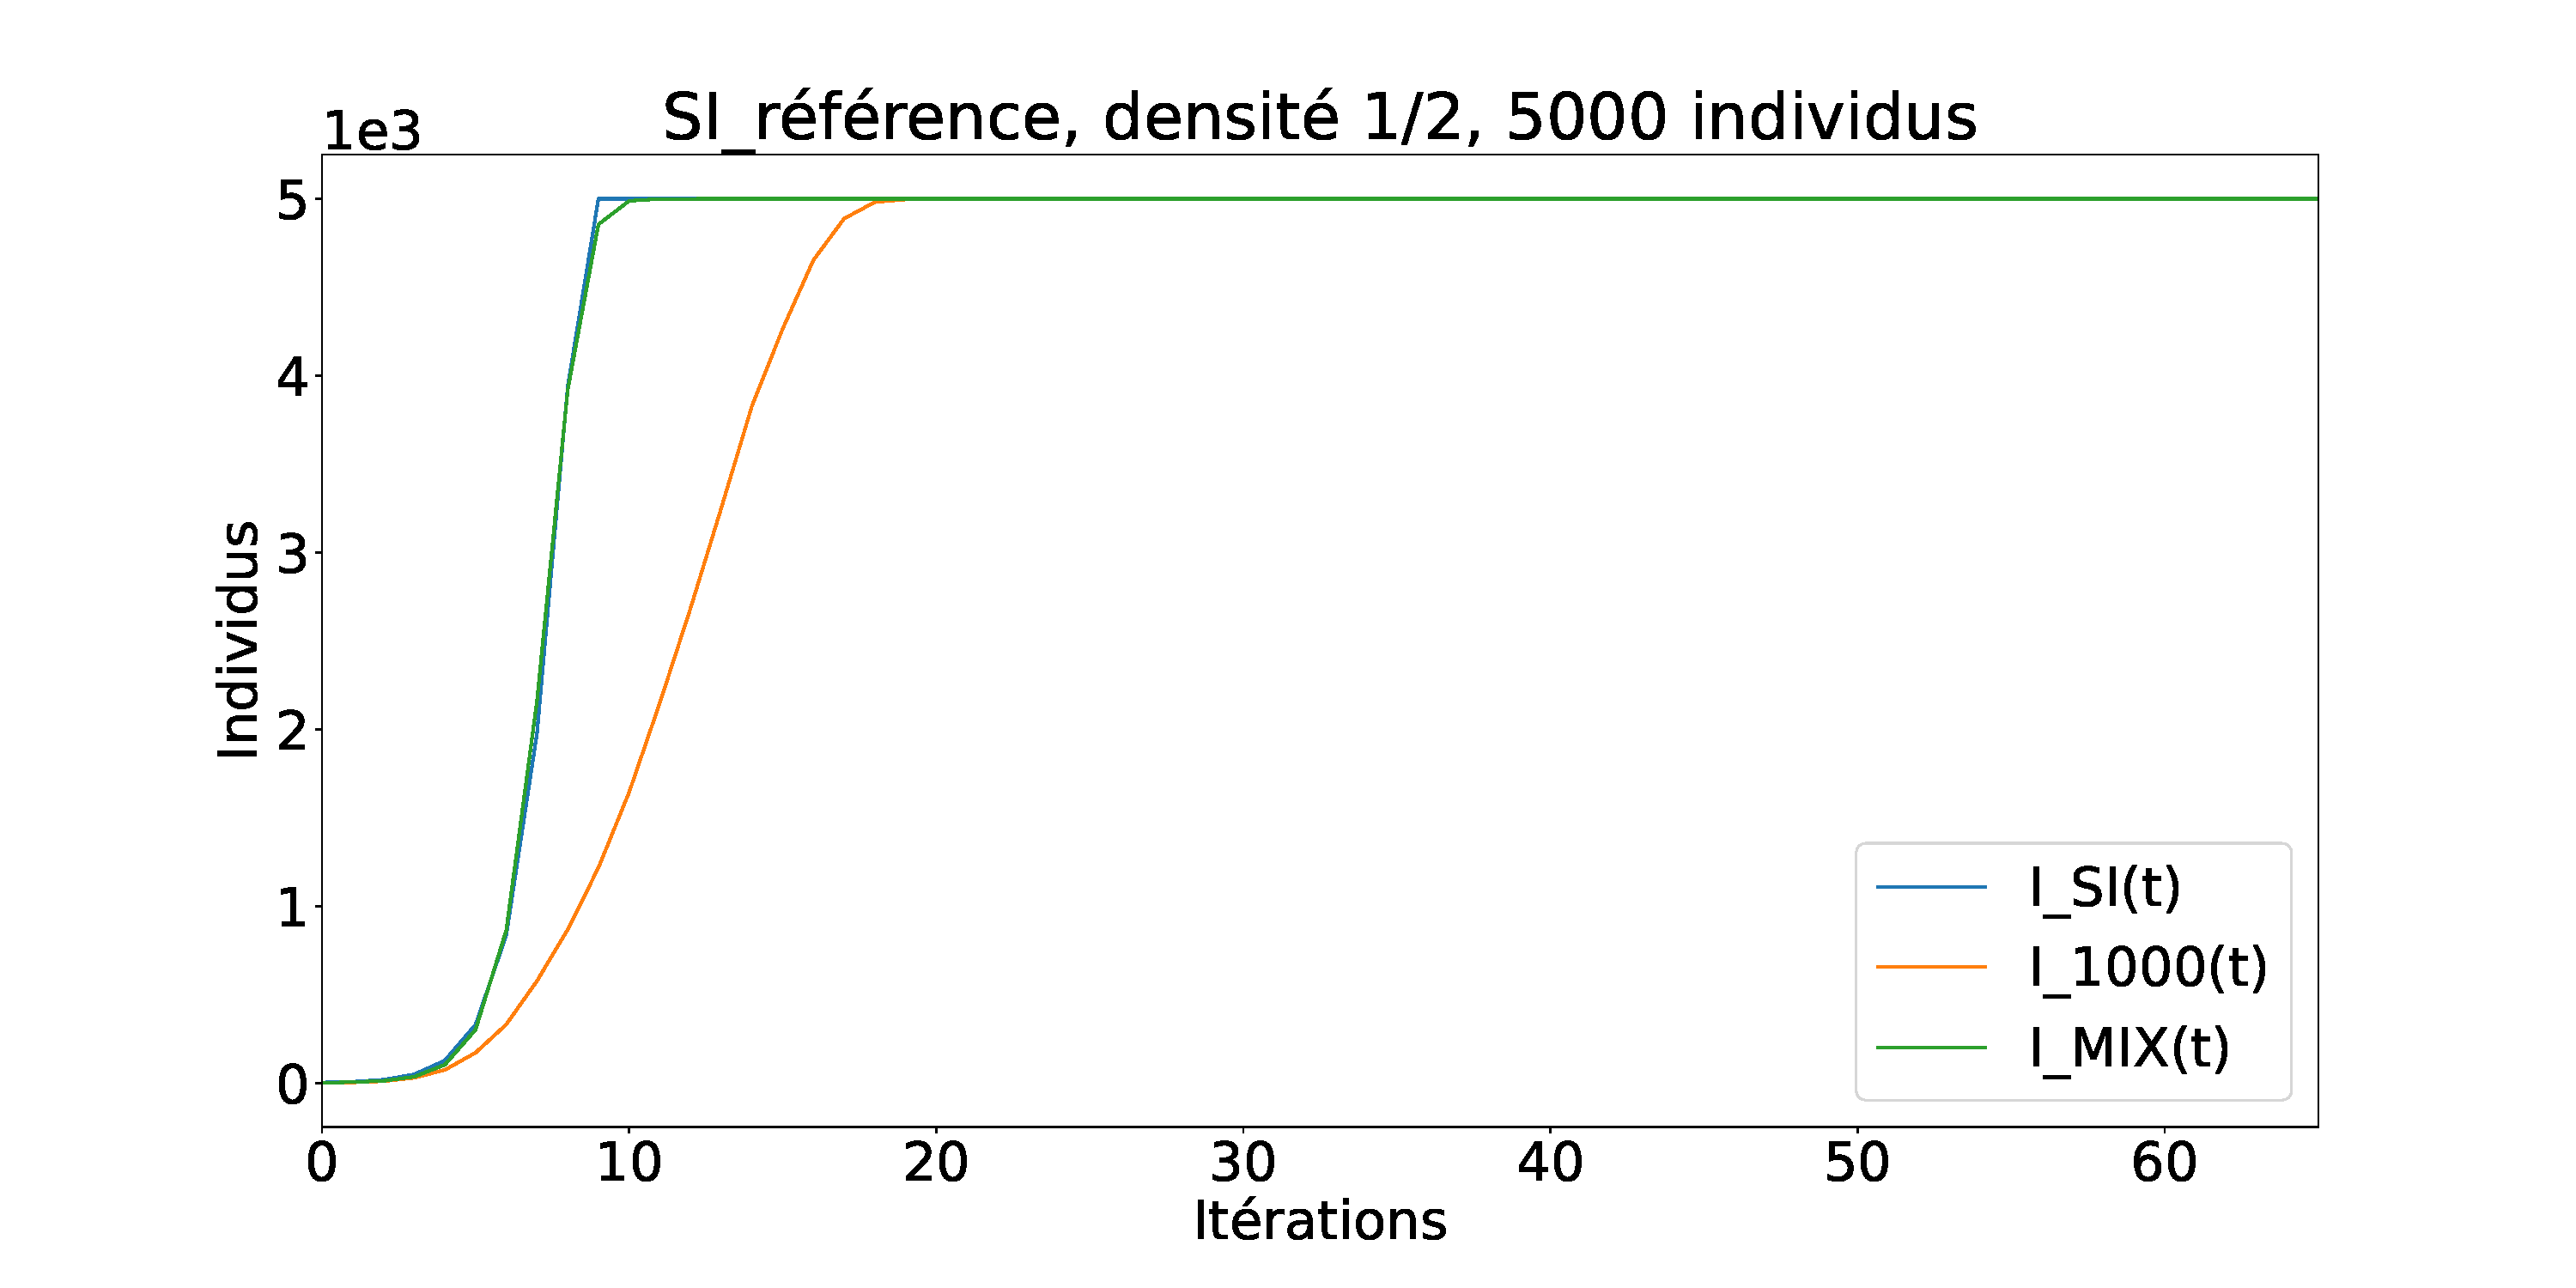
\includegraphics[width=0.5\textwidth]{Images/SI_ref_2_5k.pdf}
    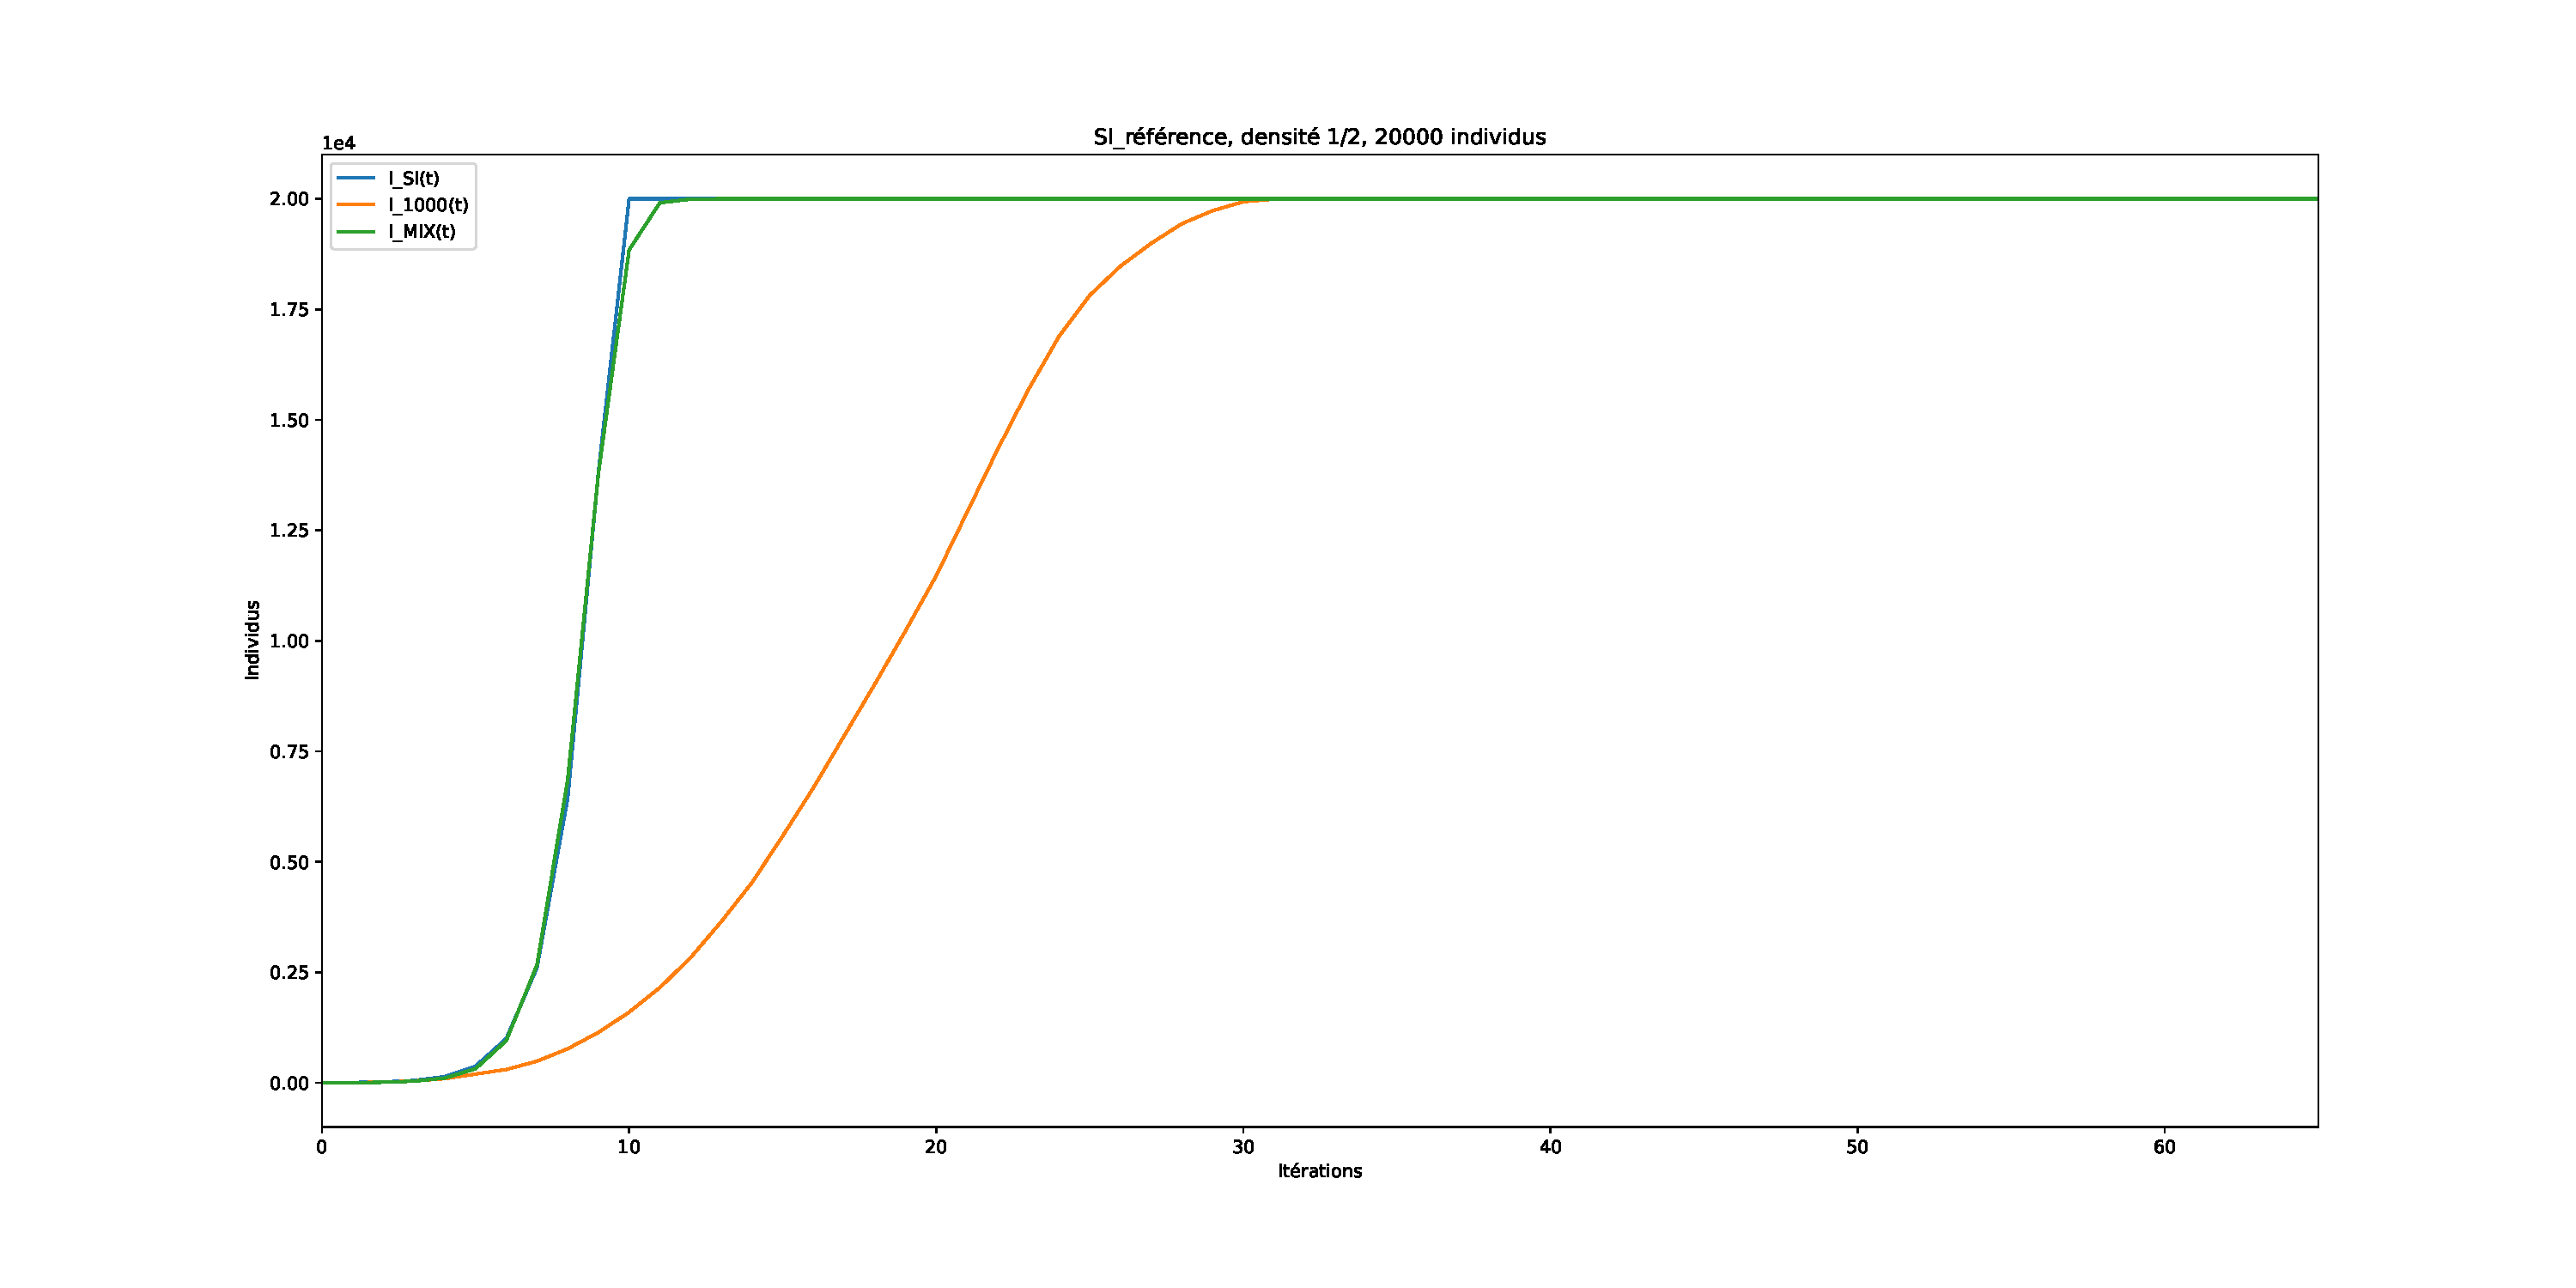
\includegraphics[width=0.5\textwidth]{Images/SI_ref_2_20k.pdf}
    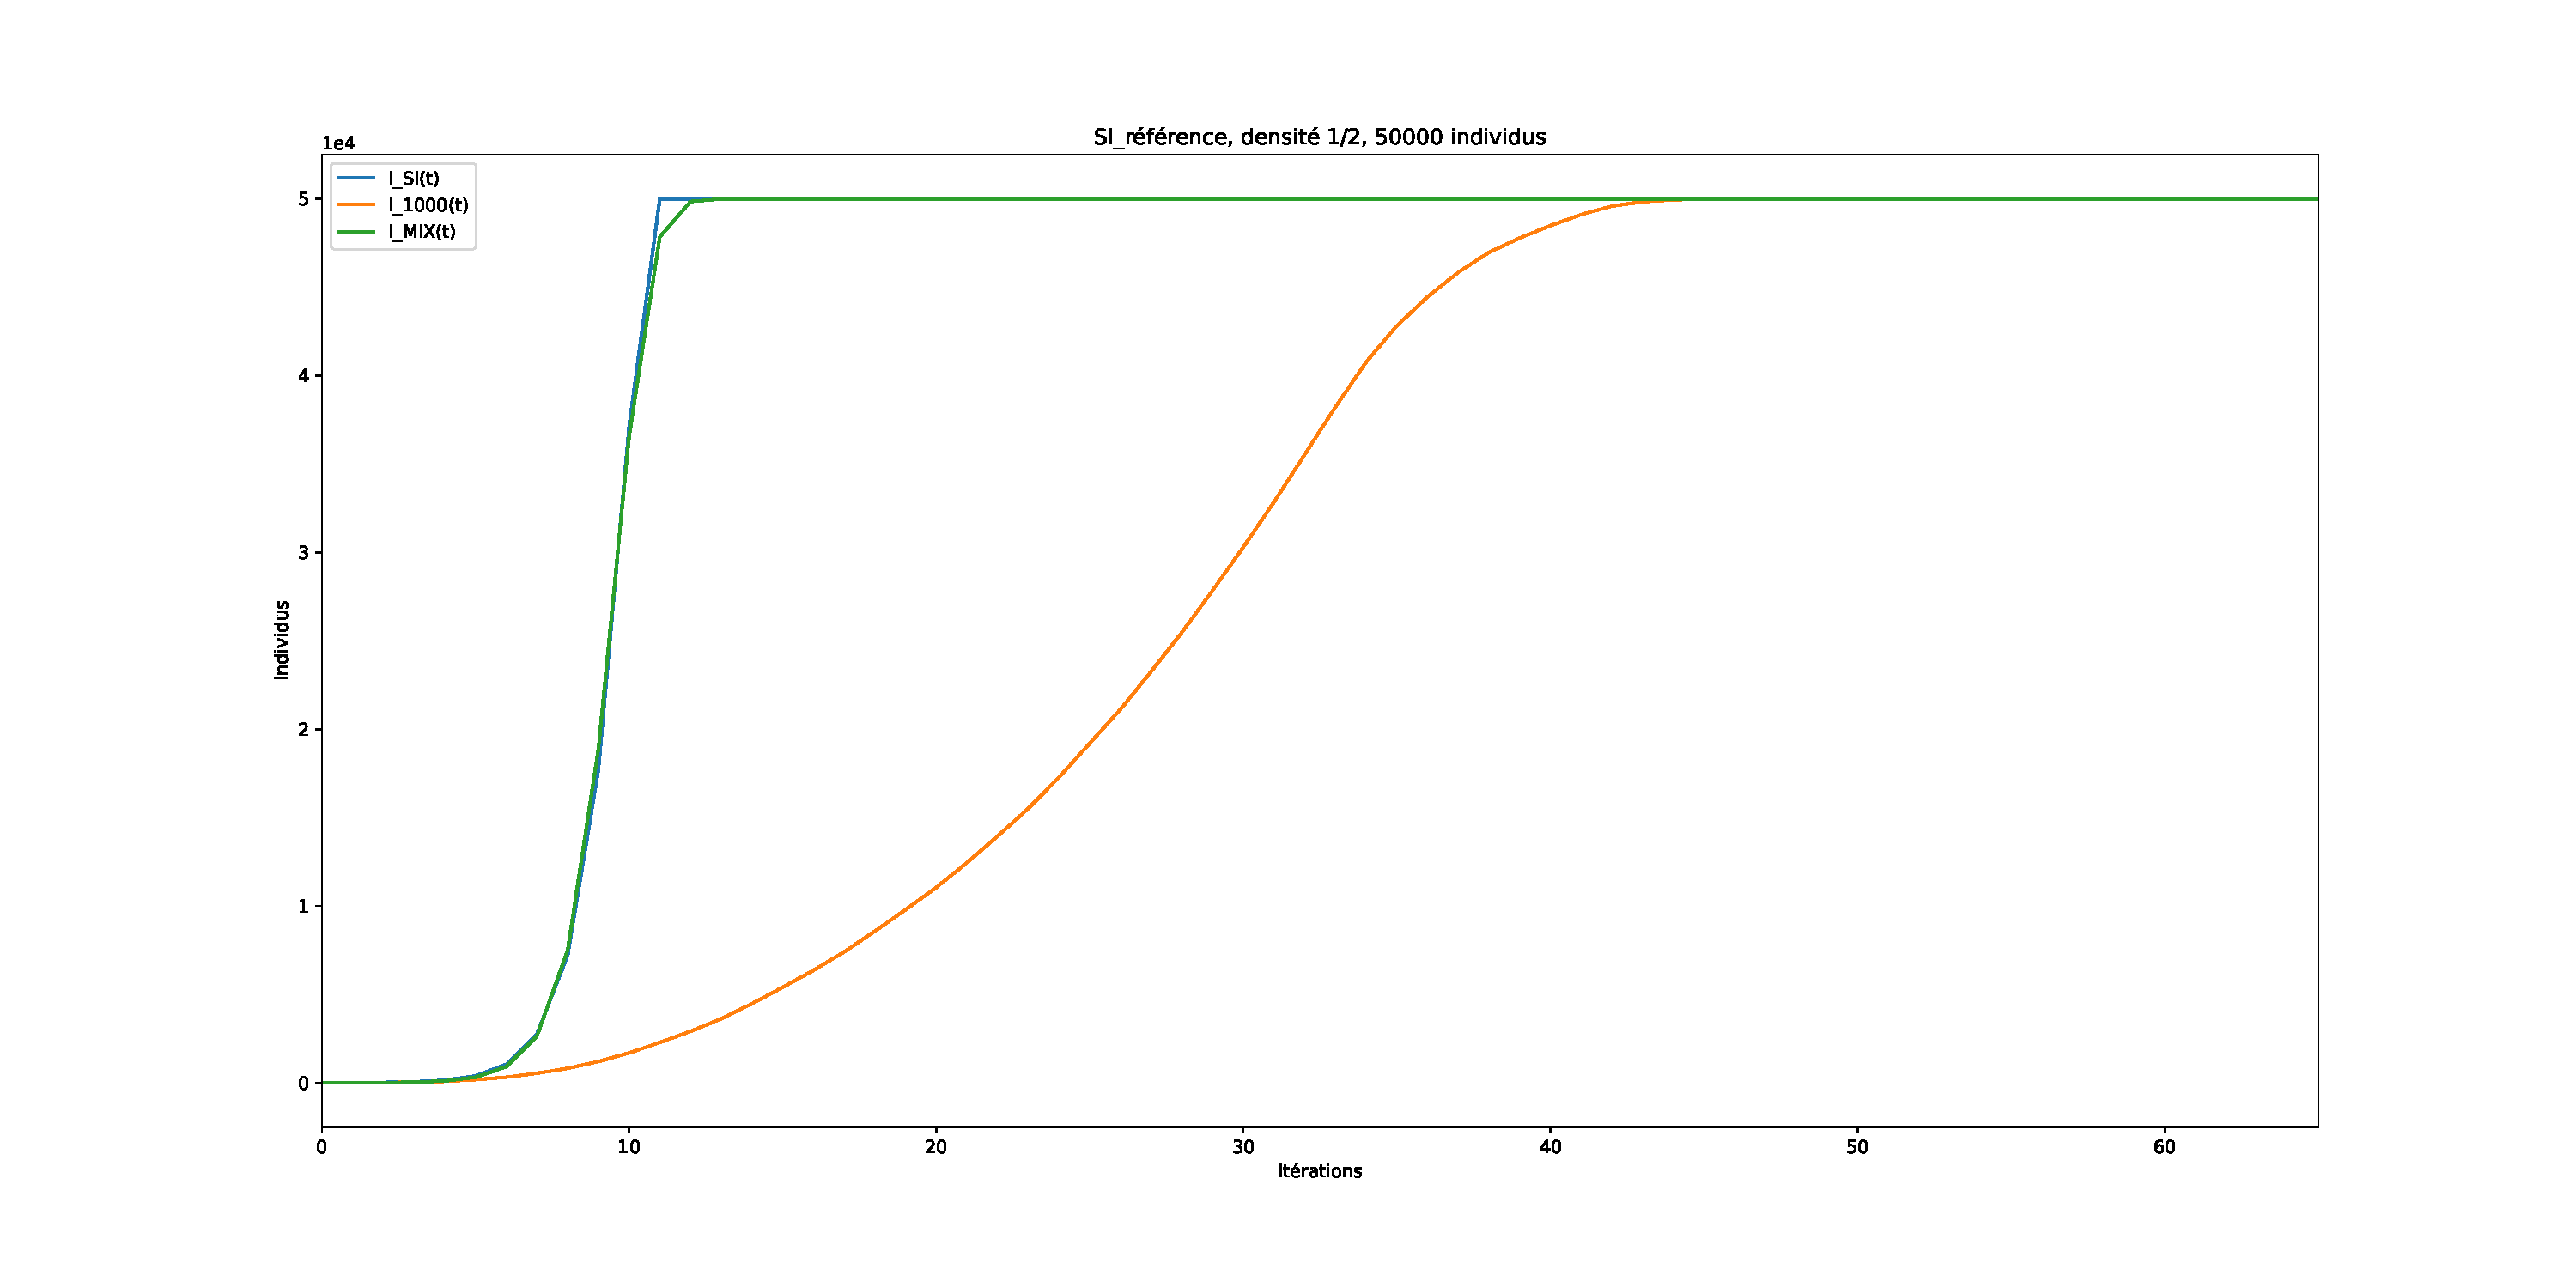
\includegraphics[width=0.5\textwidth]{Images/SI_ref_2_50k.pdf}
    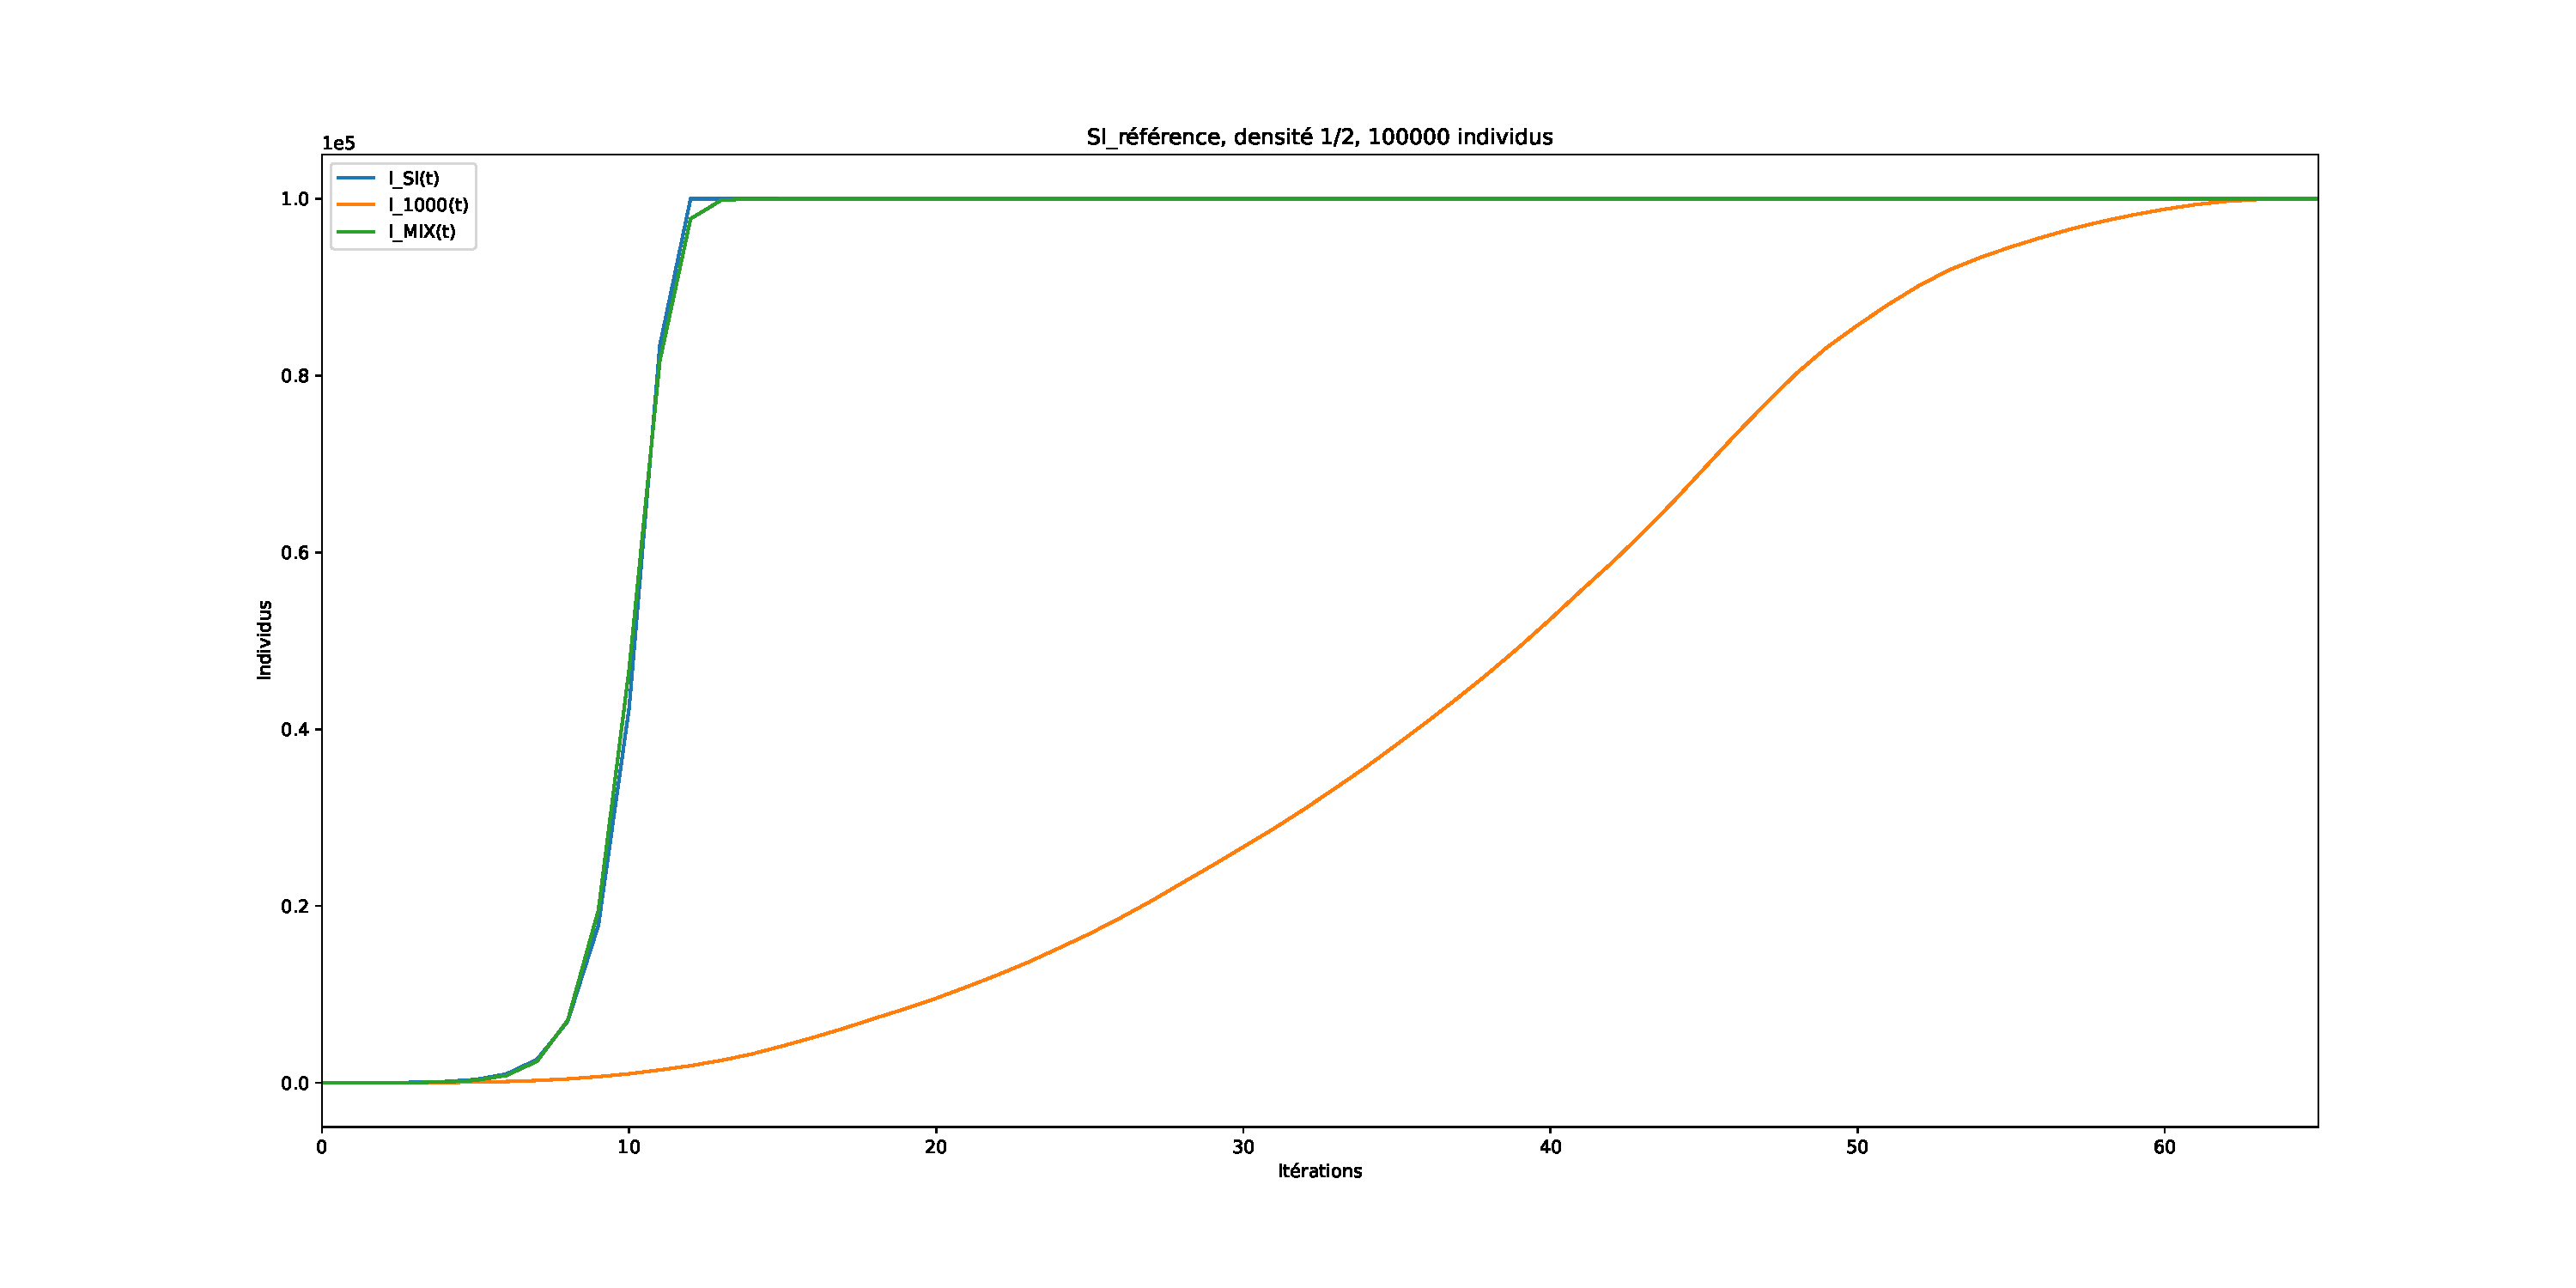
\includegraphics[width=0.5\textwidth]{Images/SI_ref_2_100k.pdf}
    \caption{Simulations de SI, densité 1/2}
\end{wrapfigure}

Le modèle est très précis pour des systèmes très denses. Les similitudes entre les courbes du modèle SI et celle du mélange parfait montrent que le modèle suit les mêmes comportements que ceux du modèle mathématique SI. Le déroulement des simulations sur des systèmes denses sont presque déterministes car elles produisent toujours les mêmes résultats sans variations apparentes. Ceci est dû au fait que pour des systèmes à forte densité, le facteur chance de déclencher un événement est plus faible que sur les systèmes moins denses. Un chapitre ultérieur est dédié à ces variations. Sur les quatre figures nous voyons sans ambiguïté que les simulations aux $1000$ mouvements (orange) déclenchent leur pandémies moins rapidement et moins brusquement. Deux phénomènes causent ces différences. \\

Le premier est dû au fait que le système est très dense. En densité $\frac{1}{2}$, la moitié des cellules du systèmes sont occupées par un un individu. Par conséquent ces derniers ont le la peine à se déplacer car ils se gênent les uns les autres dans leurs déplacements. Sans oublier que un individu, dans ces simulations, essaie de se déplacer $1000$ fois ce qui ne signifie pas qu'il se déplace effectivement $1000$ fois. Nous observons donc du retard comparé au modèle SI pour les simulations aux $1000$ mouvements. \\

Le deuxième phénomène qui explique le retard croissant est que pour toutes les simulations, le nombre de déplacements pour est constant. Par conséquent les grands systèmes se mélangent moins relativement à leur taille que les plus petits. C'est la raison pour laquelle les courbes oranges s'aplatissent de plus en plus sur des systèmes de plus en plus grands.\\

\newpage

\begin{wrapfigure}{r}{0.5\textwidth}
    \centering
    \captionsetup{justification=centering}
    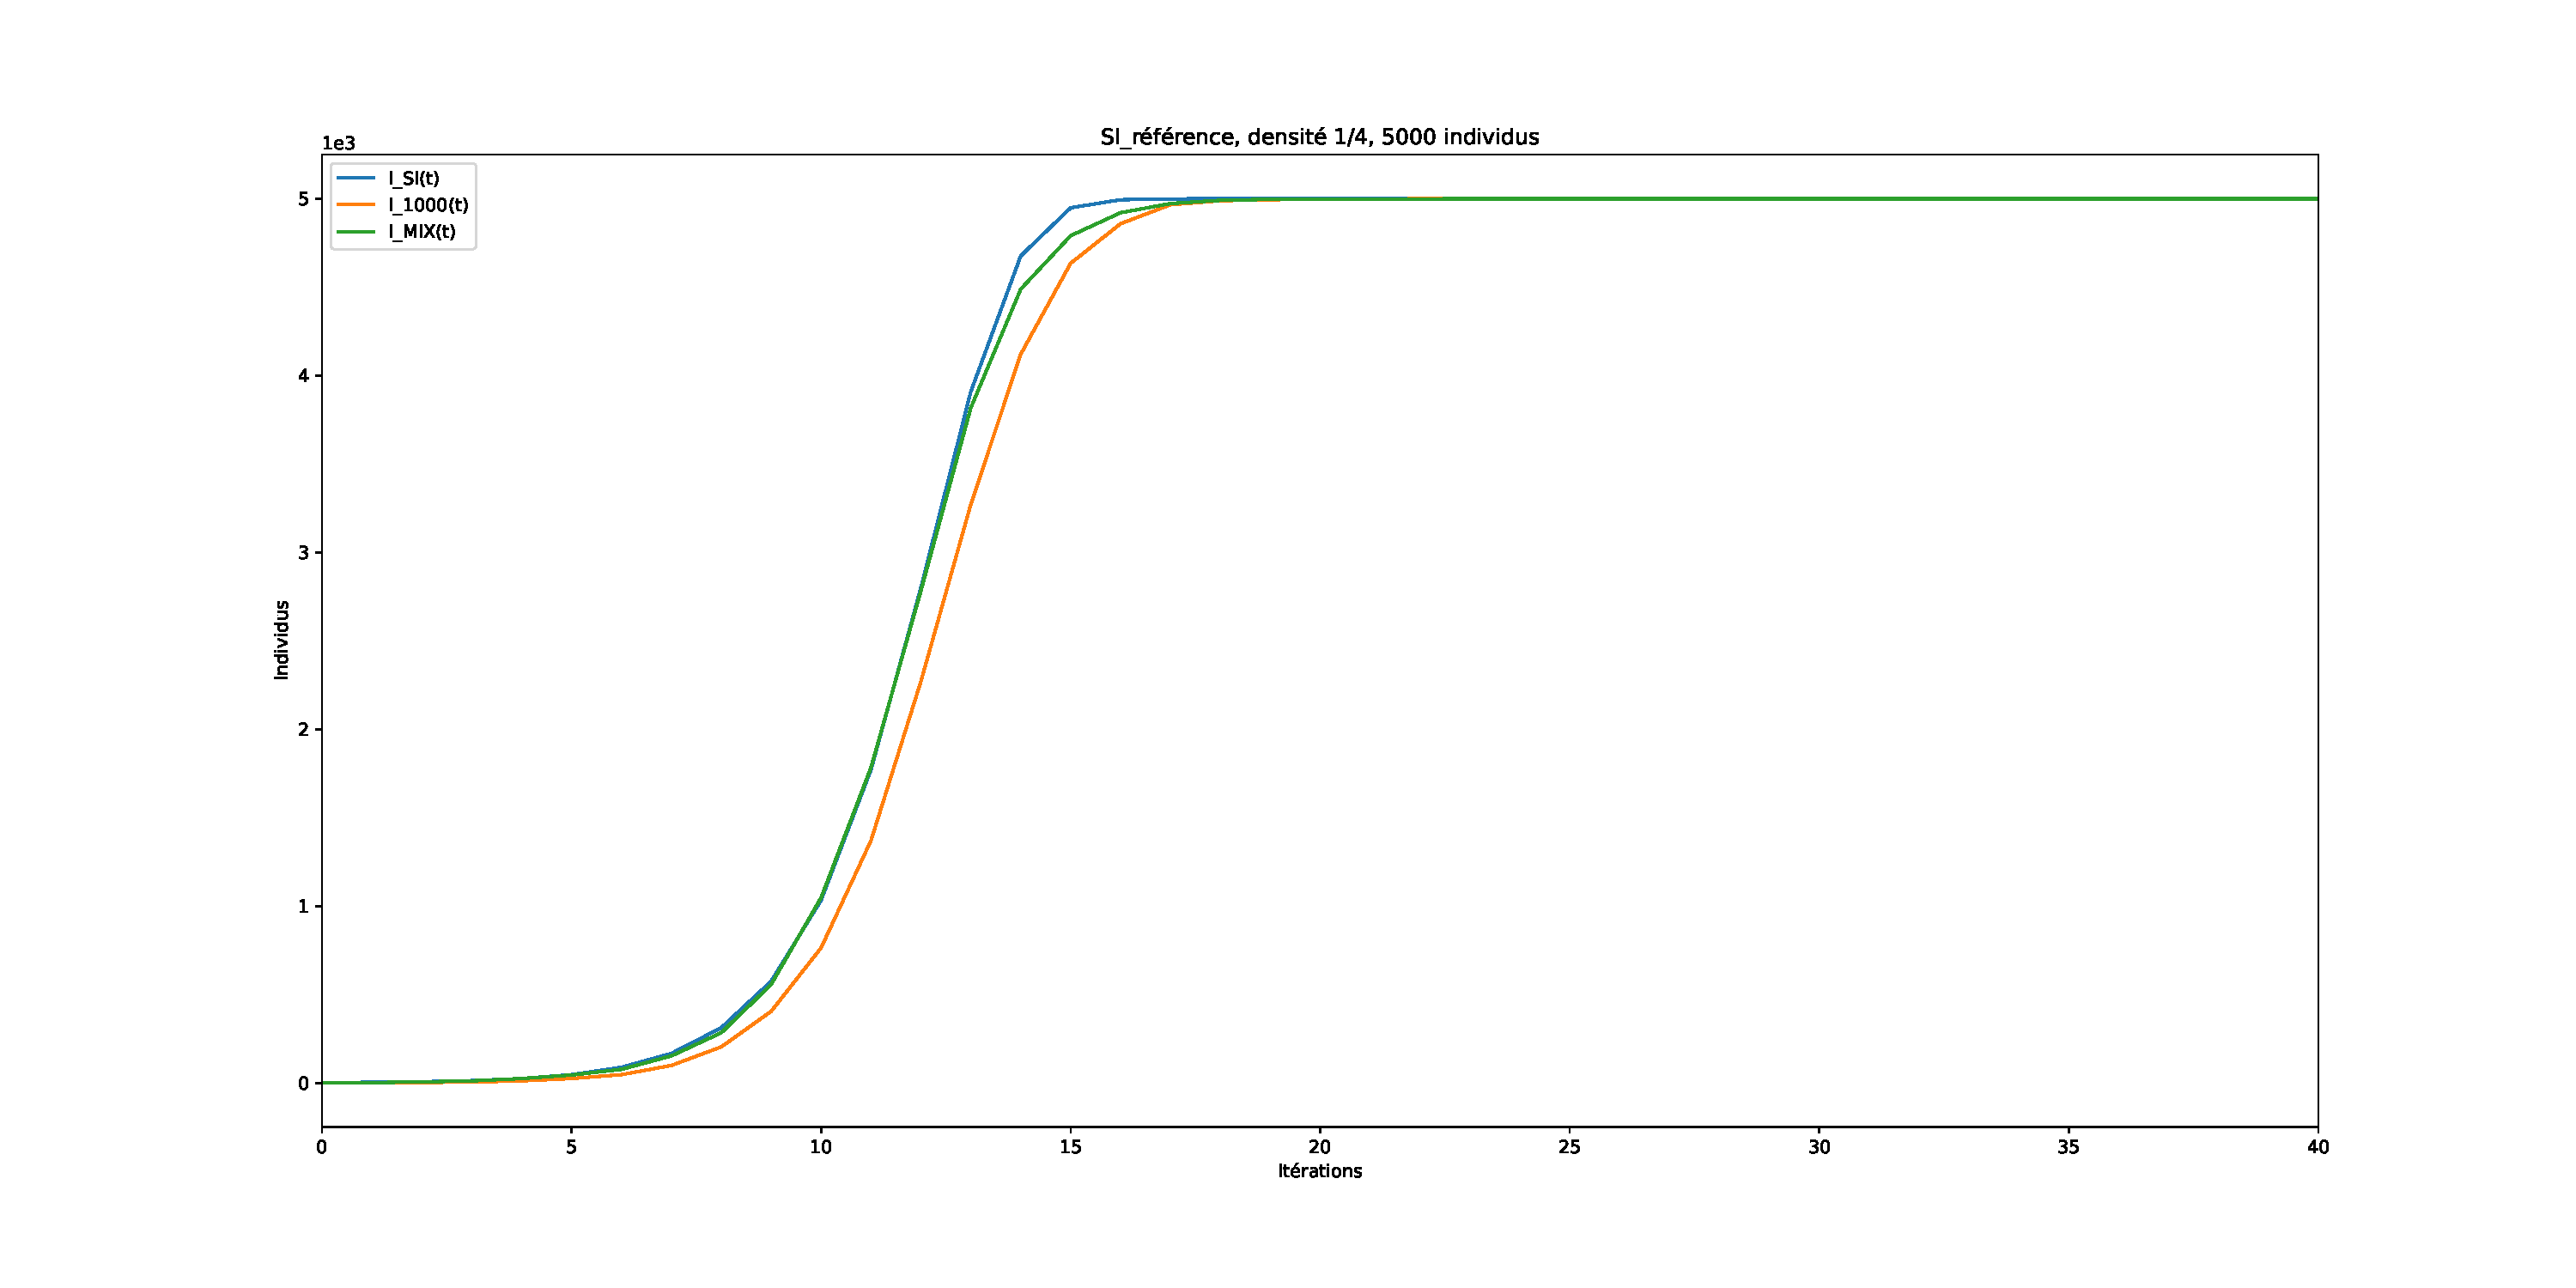
\includegraphics[width=0.5\textwidth]{Images/SI_ref_4_5k.pdf}
    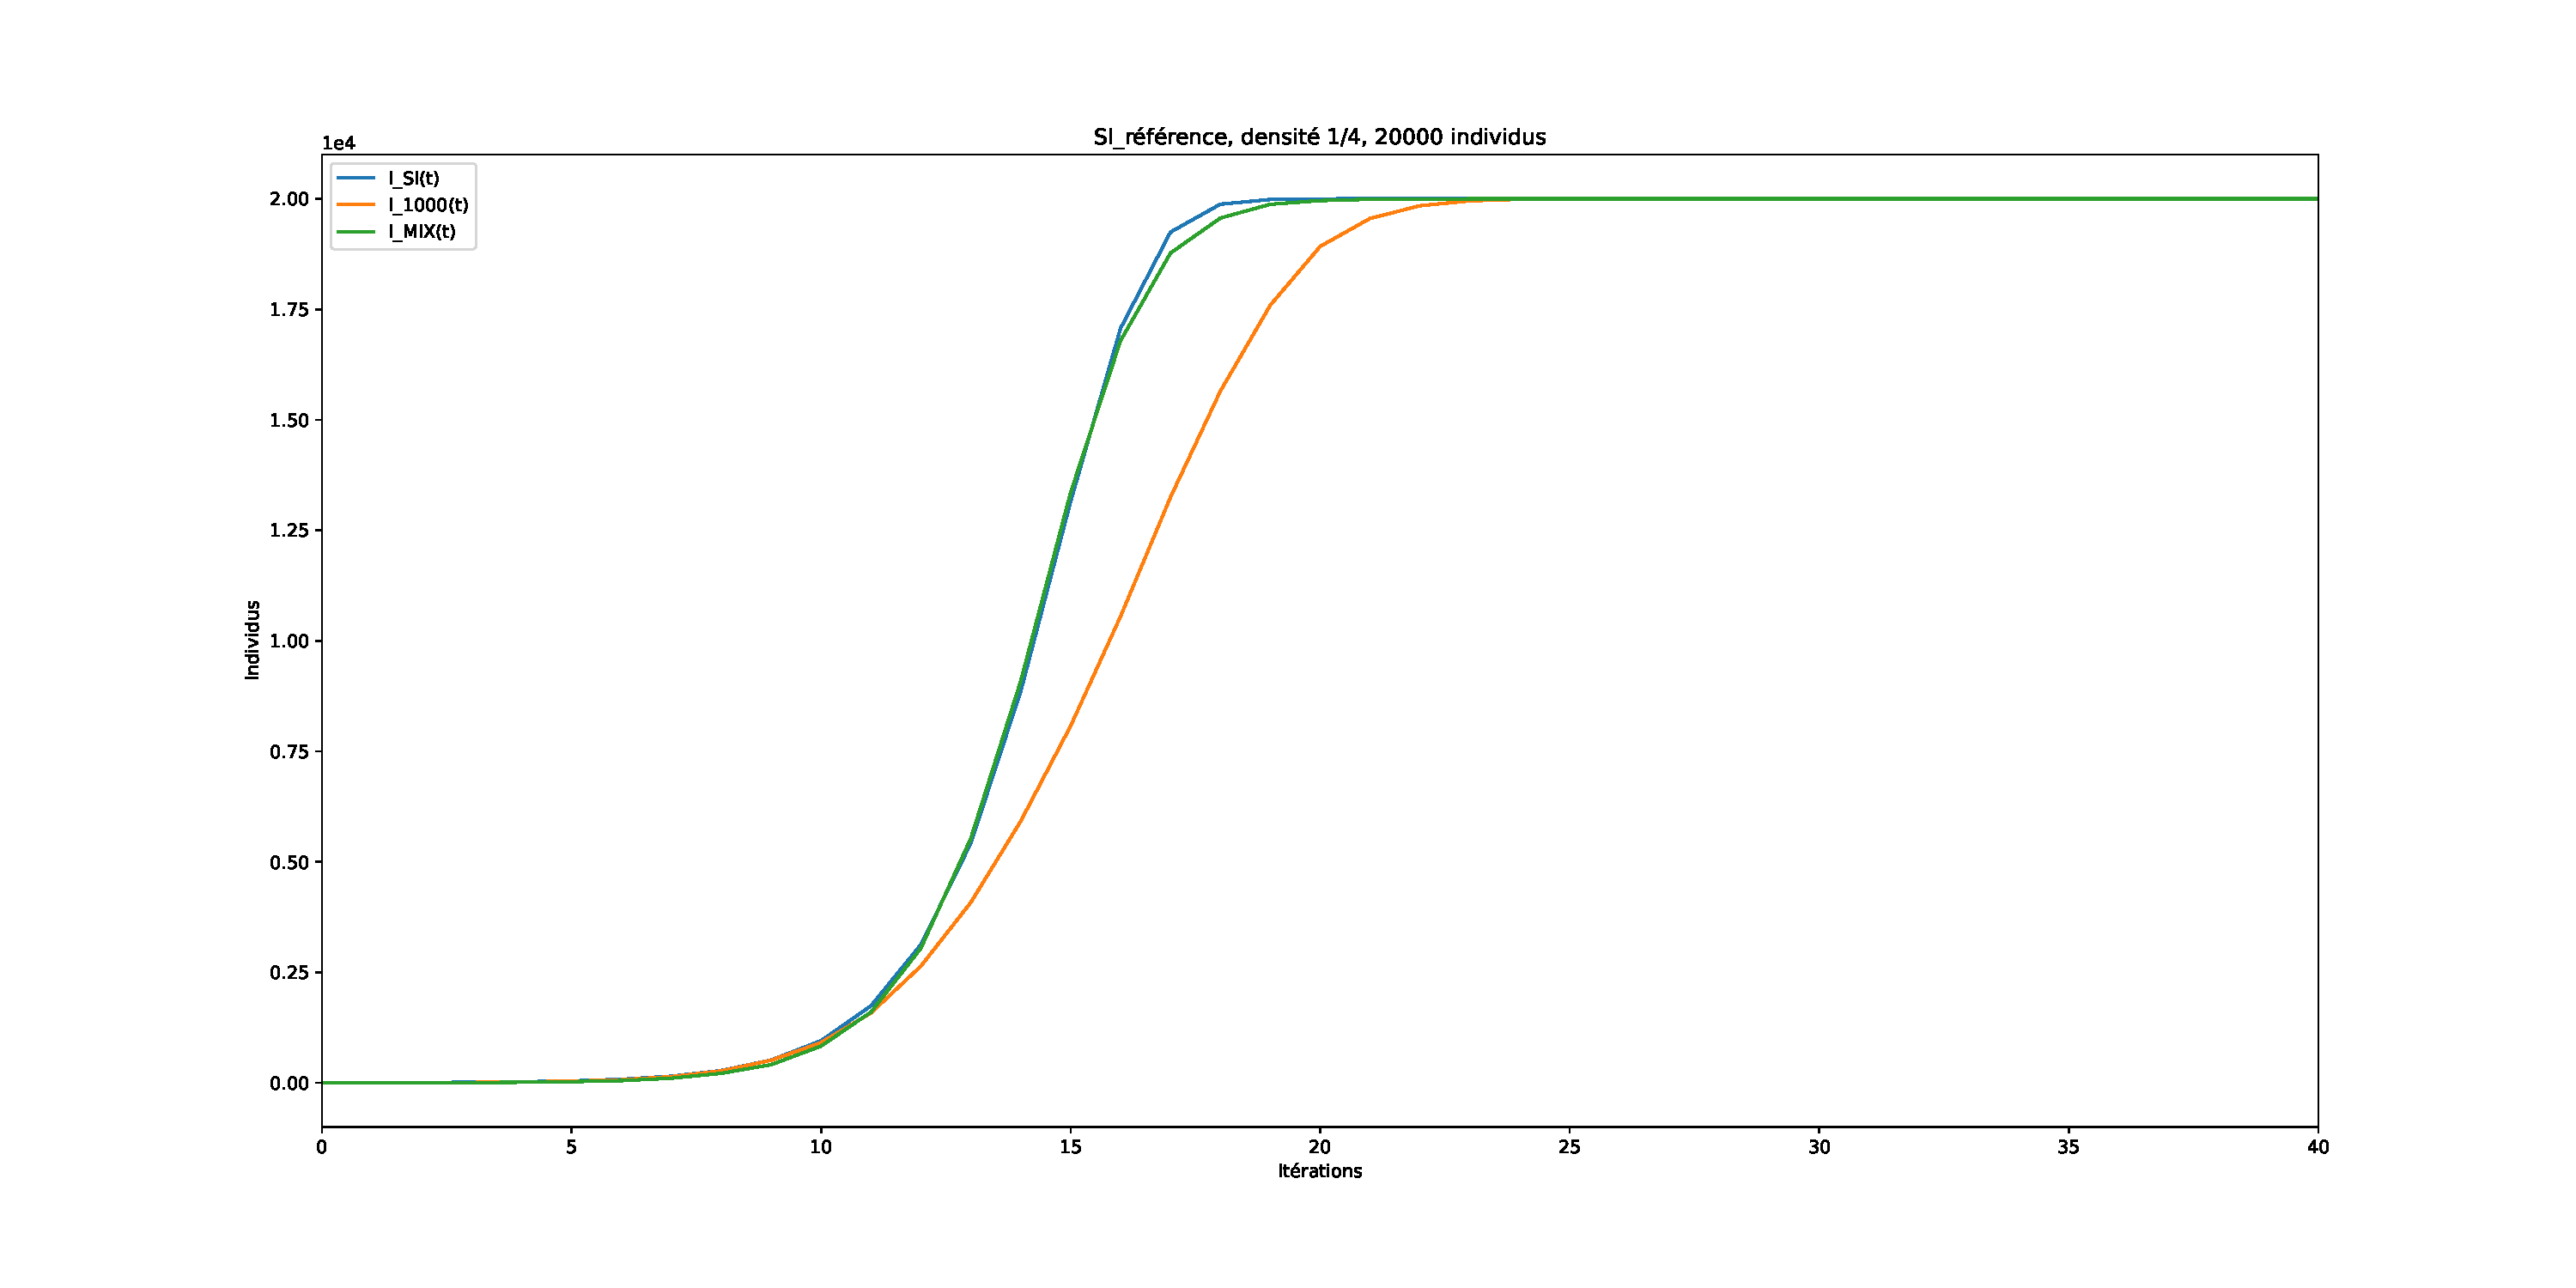
\includegraphics[width=0.5\textwidth]{Images/SI_ref_4_20k.pdf}
    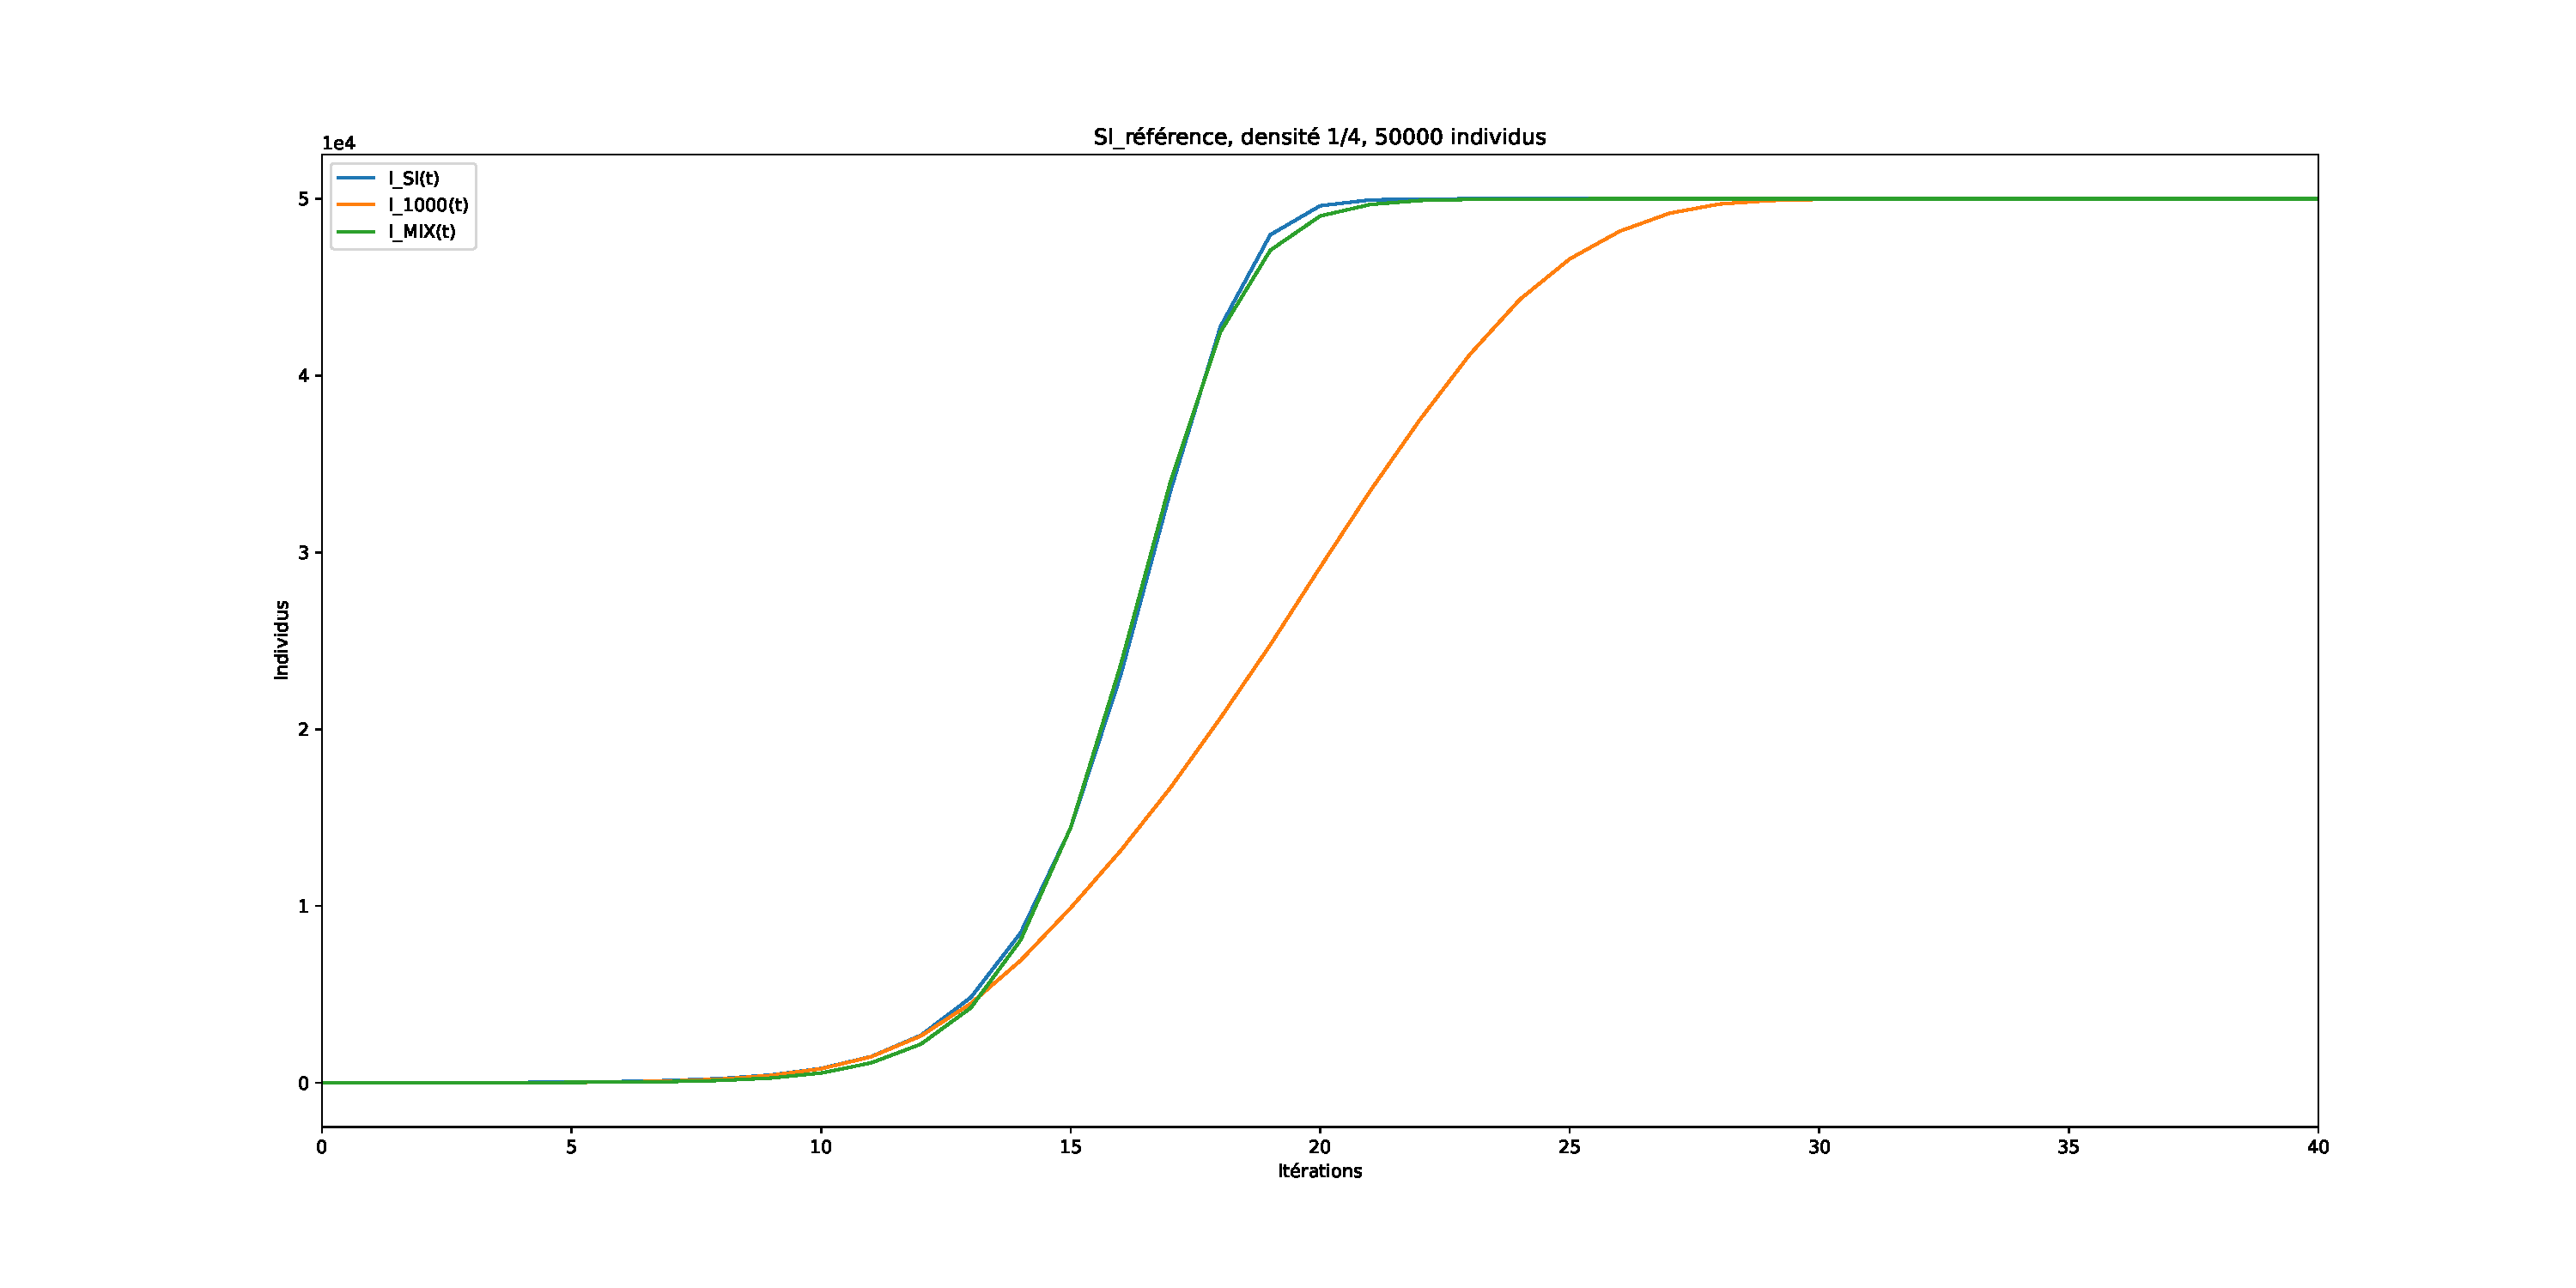
\includegraphics[width=0.5\textwidth]{Images/SI_ref_4_50k.pdf}
    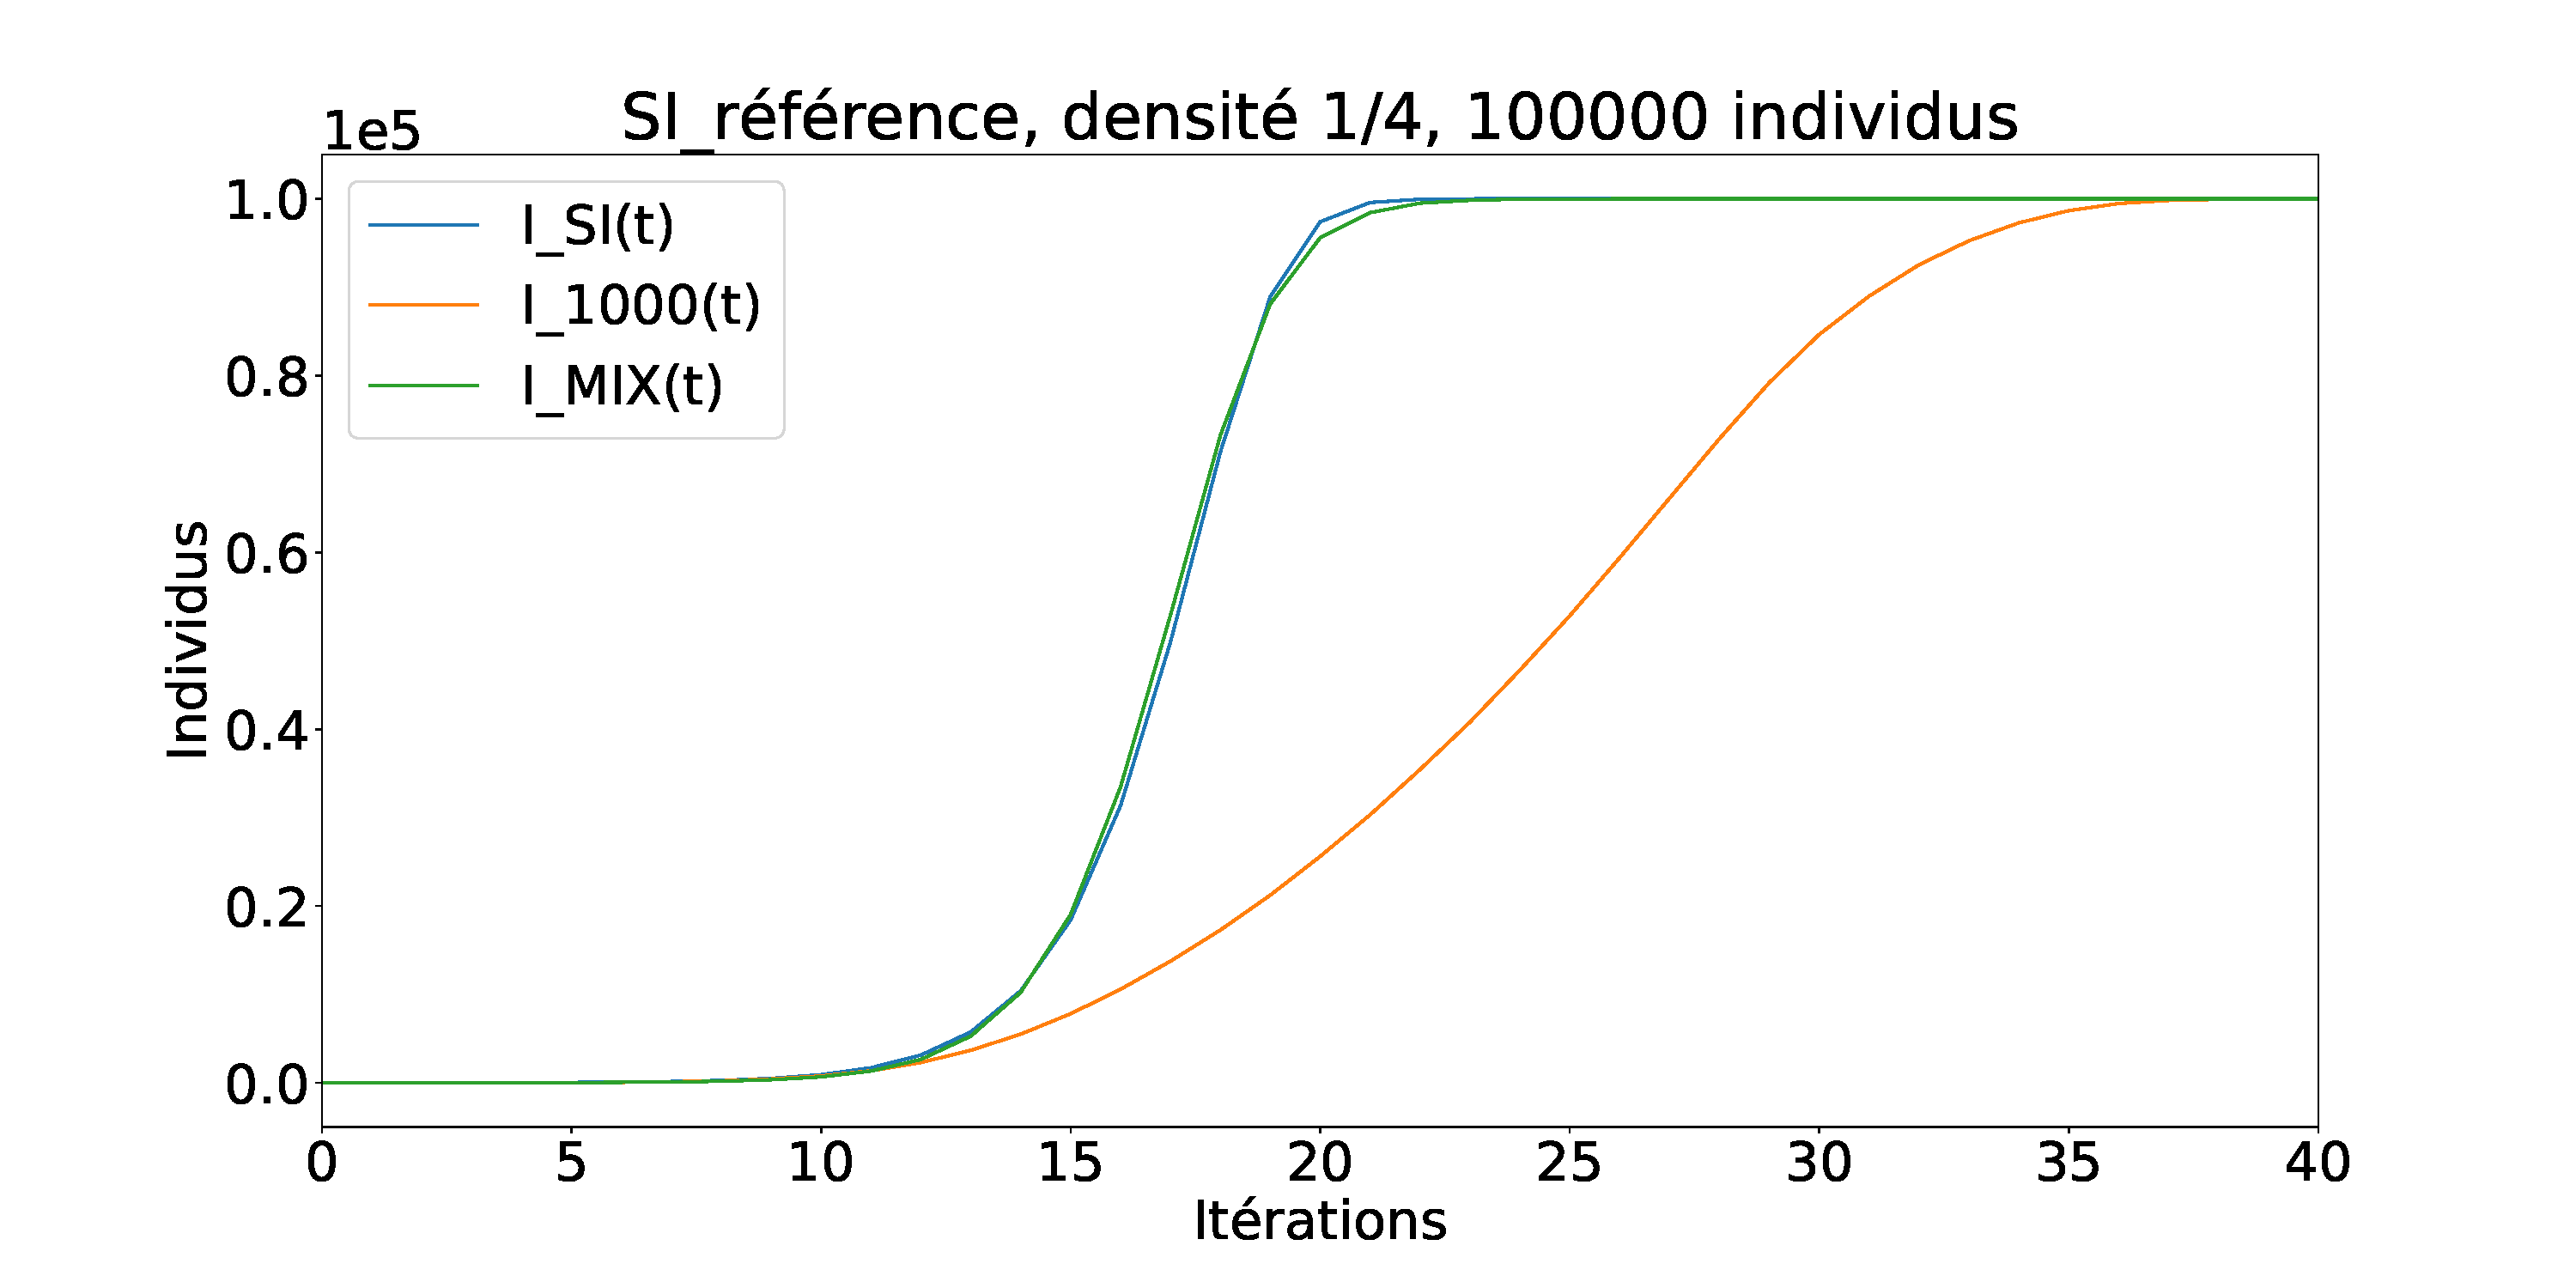
\includegraphics[width=0.5\textwidth]{Images/SI_ref_4_100k.pdf}
    \caption{Simulations de SI, densité 1/4}
\end{wrapfigure}

Une densité de population de $\frac{1}{4}$ permet d'avantages de déplacement pour les individus, par conséquent le mélange pour la méthode à $1000$ mouvements est de meilleure qualité. Nous avons donc des courbes oranges qui subissent moins les blocages et elle approchent d'avantage le modèle SI.\\

Des résultats similaires sont observés pour une densité de $\frac{1}{4}$ que pour une densité de $\frac{1}{2}$. Une différence notable est que les coures oranges s'approchent d'avantage au mélange parfait que précédemment. Un système à cette densité reste très déterministe et par conséquent toutes les simulations au mélange parfait produisent des résultats précis qui collent au modèle SI.\\

De même pour cette densité, le taux de mélange de $1000$ mouvements fixe impacte les grands systèmes en s'éloignant du modèle SI. Par contre la simulation sur $5000$ individus particulièrement précise et ceci bien plus que les simulations en densité $\frac{1}{2}$. Ceci est dû au fait qu'une densité de $\frac{1}{4}$ permet aux acteur de se déplacer plus aisément et donc d'obtenir un meilleur mélange. Par conséquent, sur un système de taille $141\times 141$ avec $5000$ individus, le mélange des $1000$ mouvements est presque aussi bon que le mélange parfait.

\newpage

\begin{wrapfigure}{r}{0.5\textwidth}
    \centering
    \captionsetup{justification=centering}
    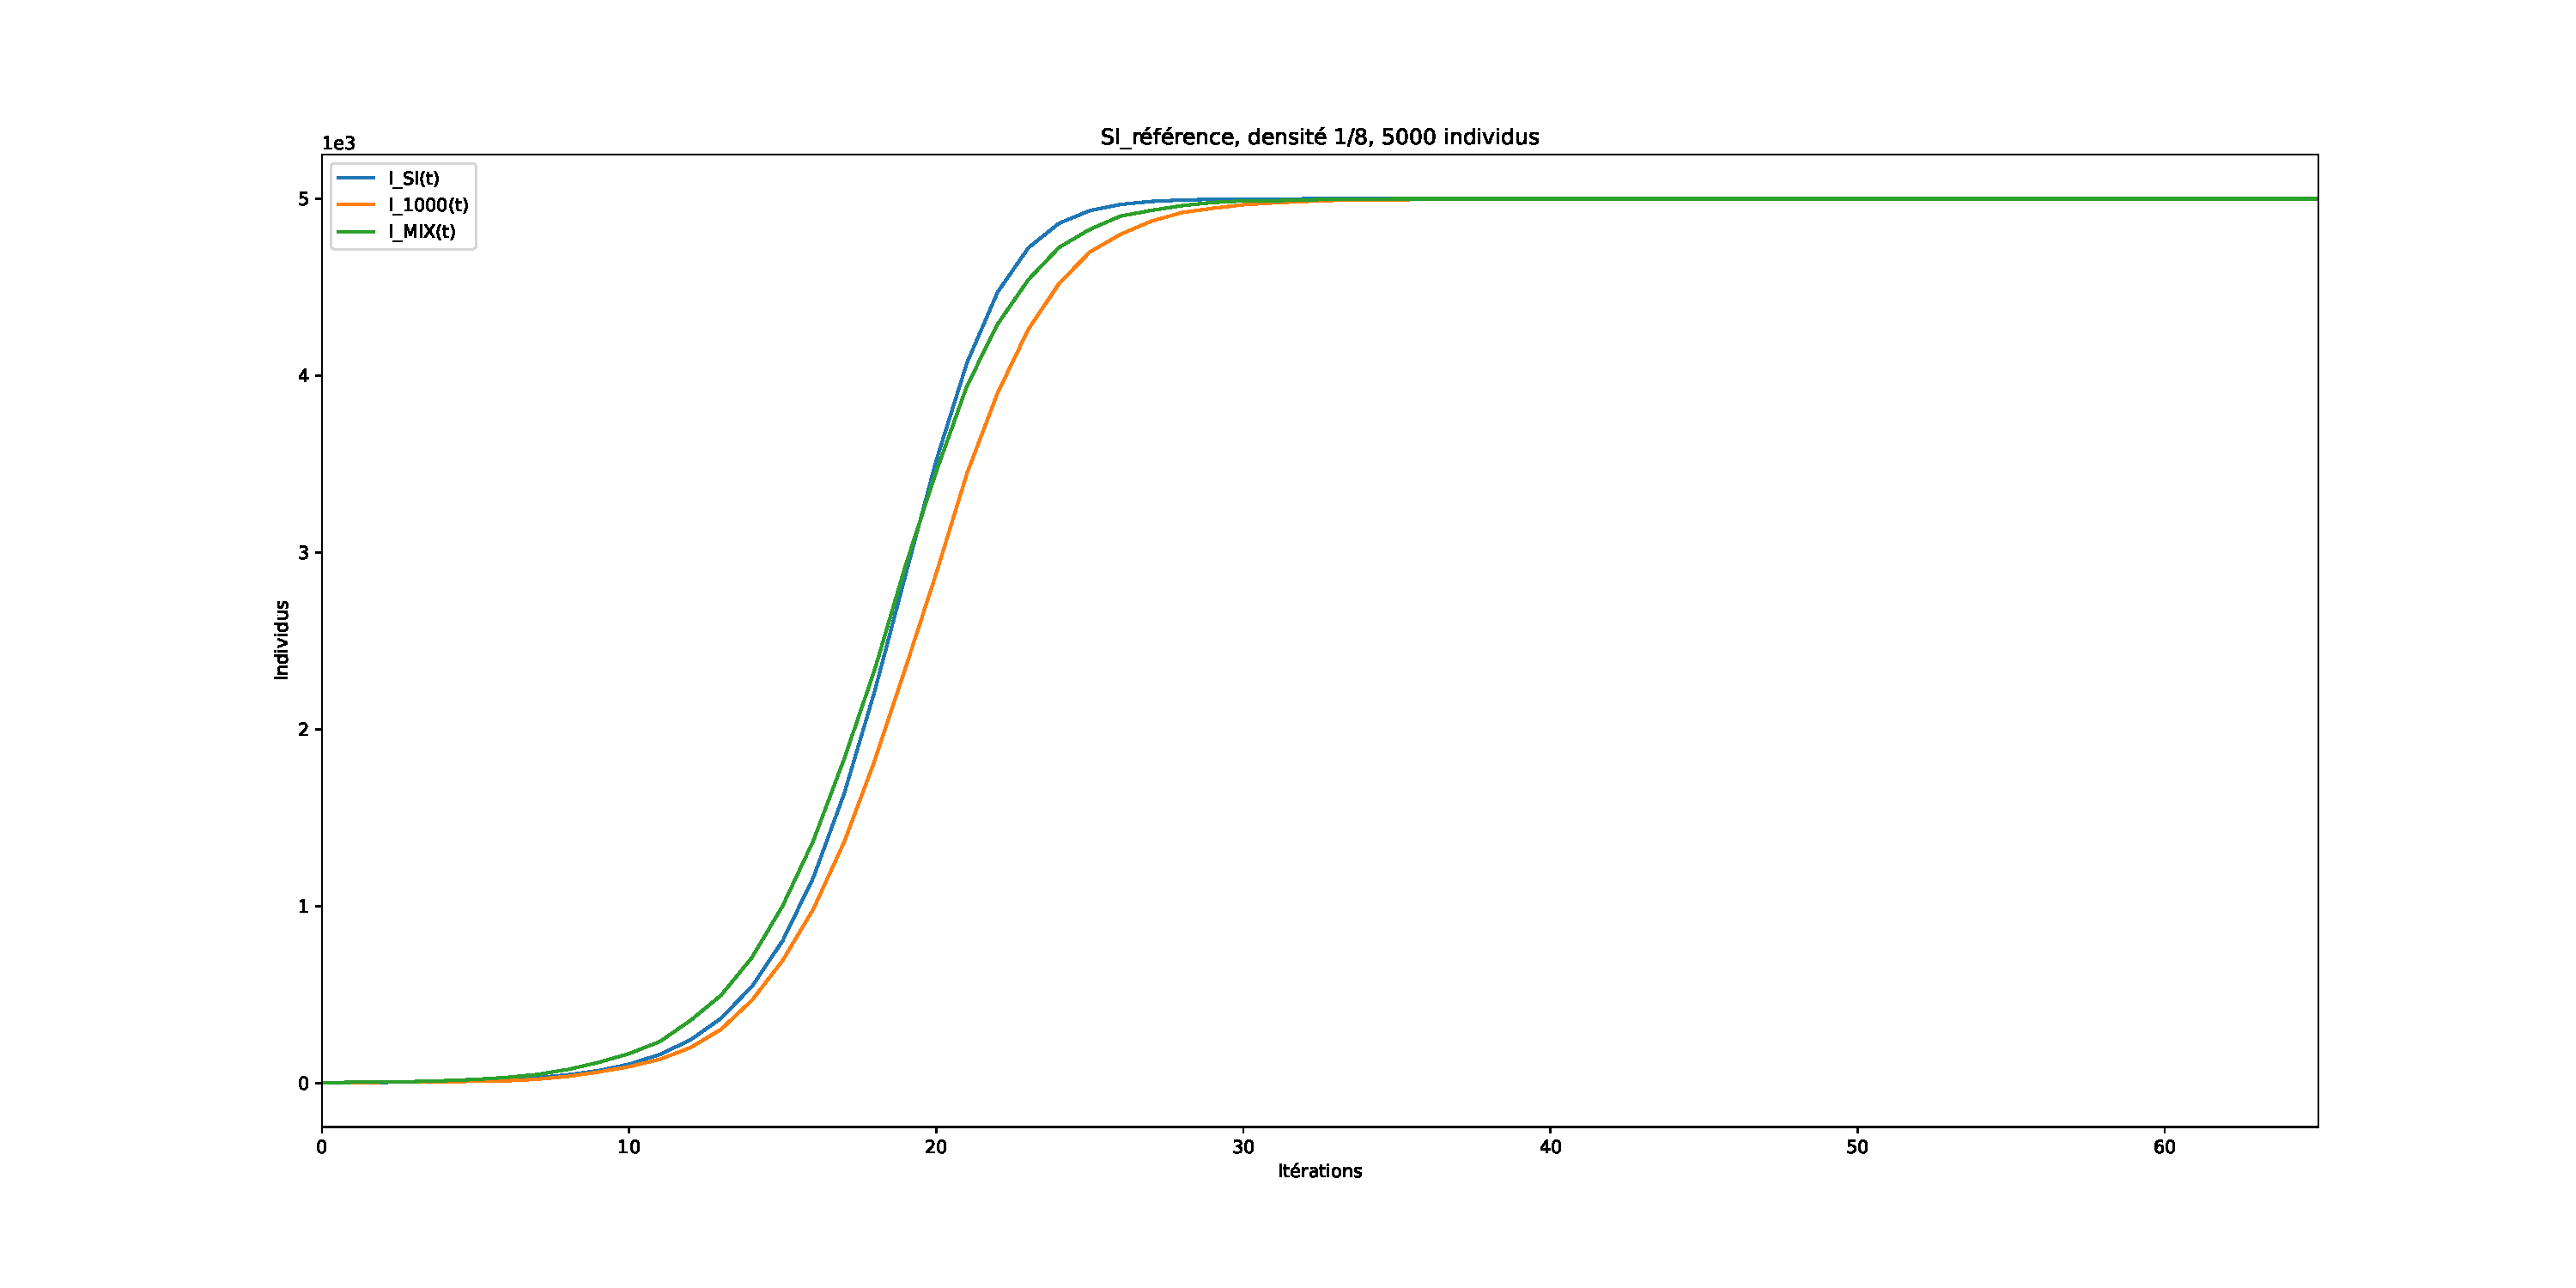
\includegraphics[width=0.5\textwidth]{Images/SI_ref_8_5k.pdf}
    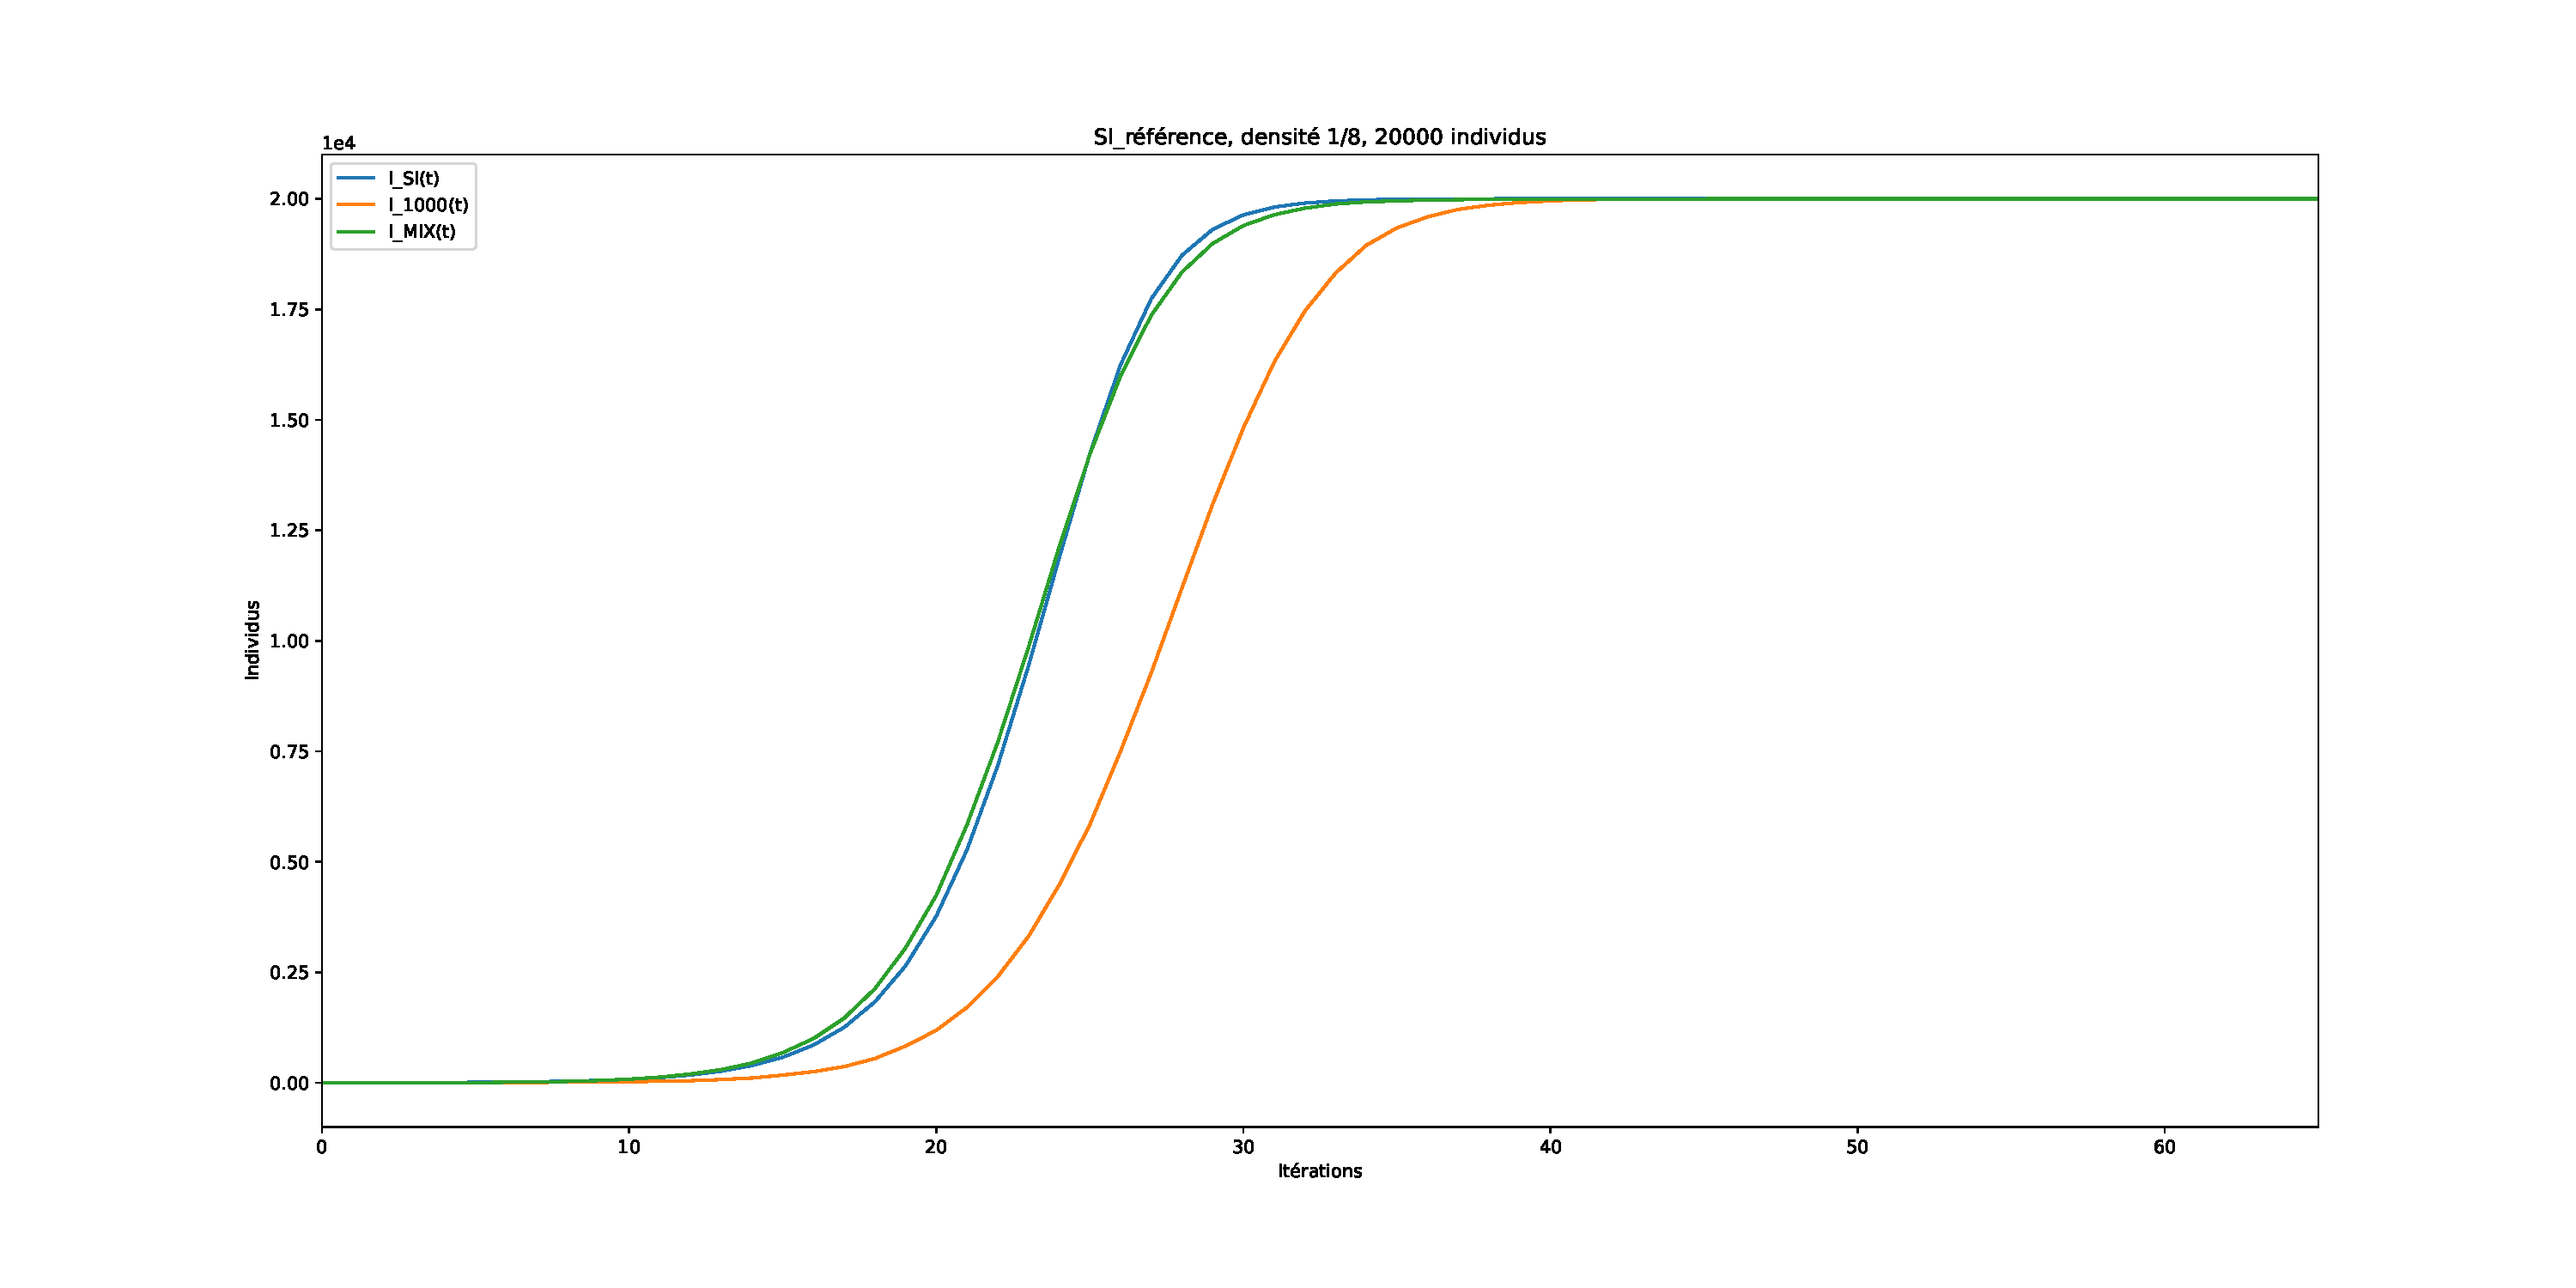
\includegraphics[width=0.5\textwidth]{Images/SI_ref_8_20k.pdf}
    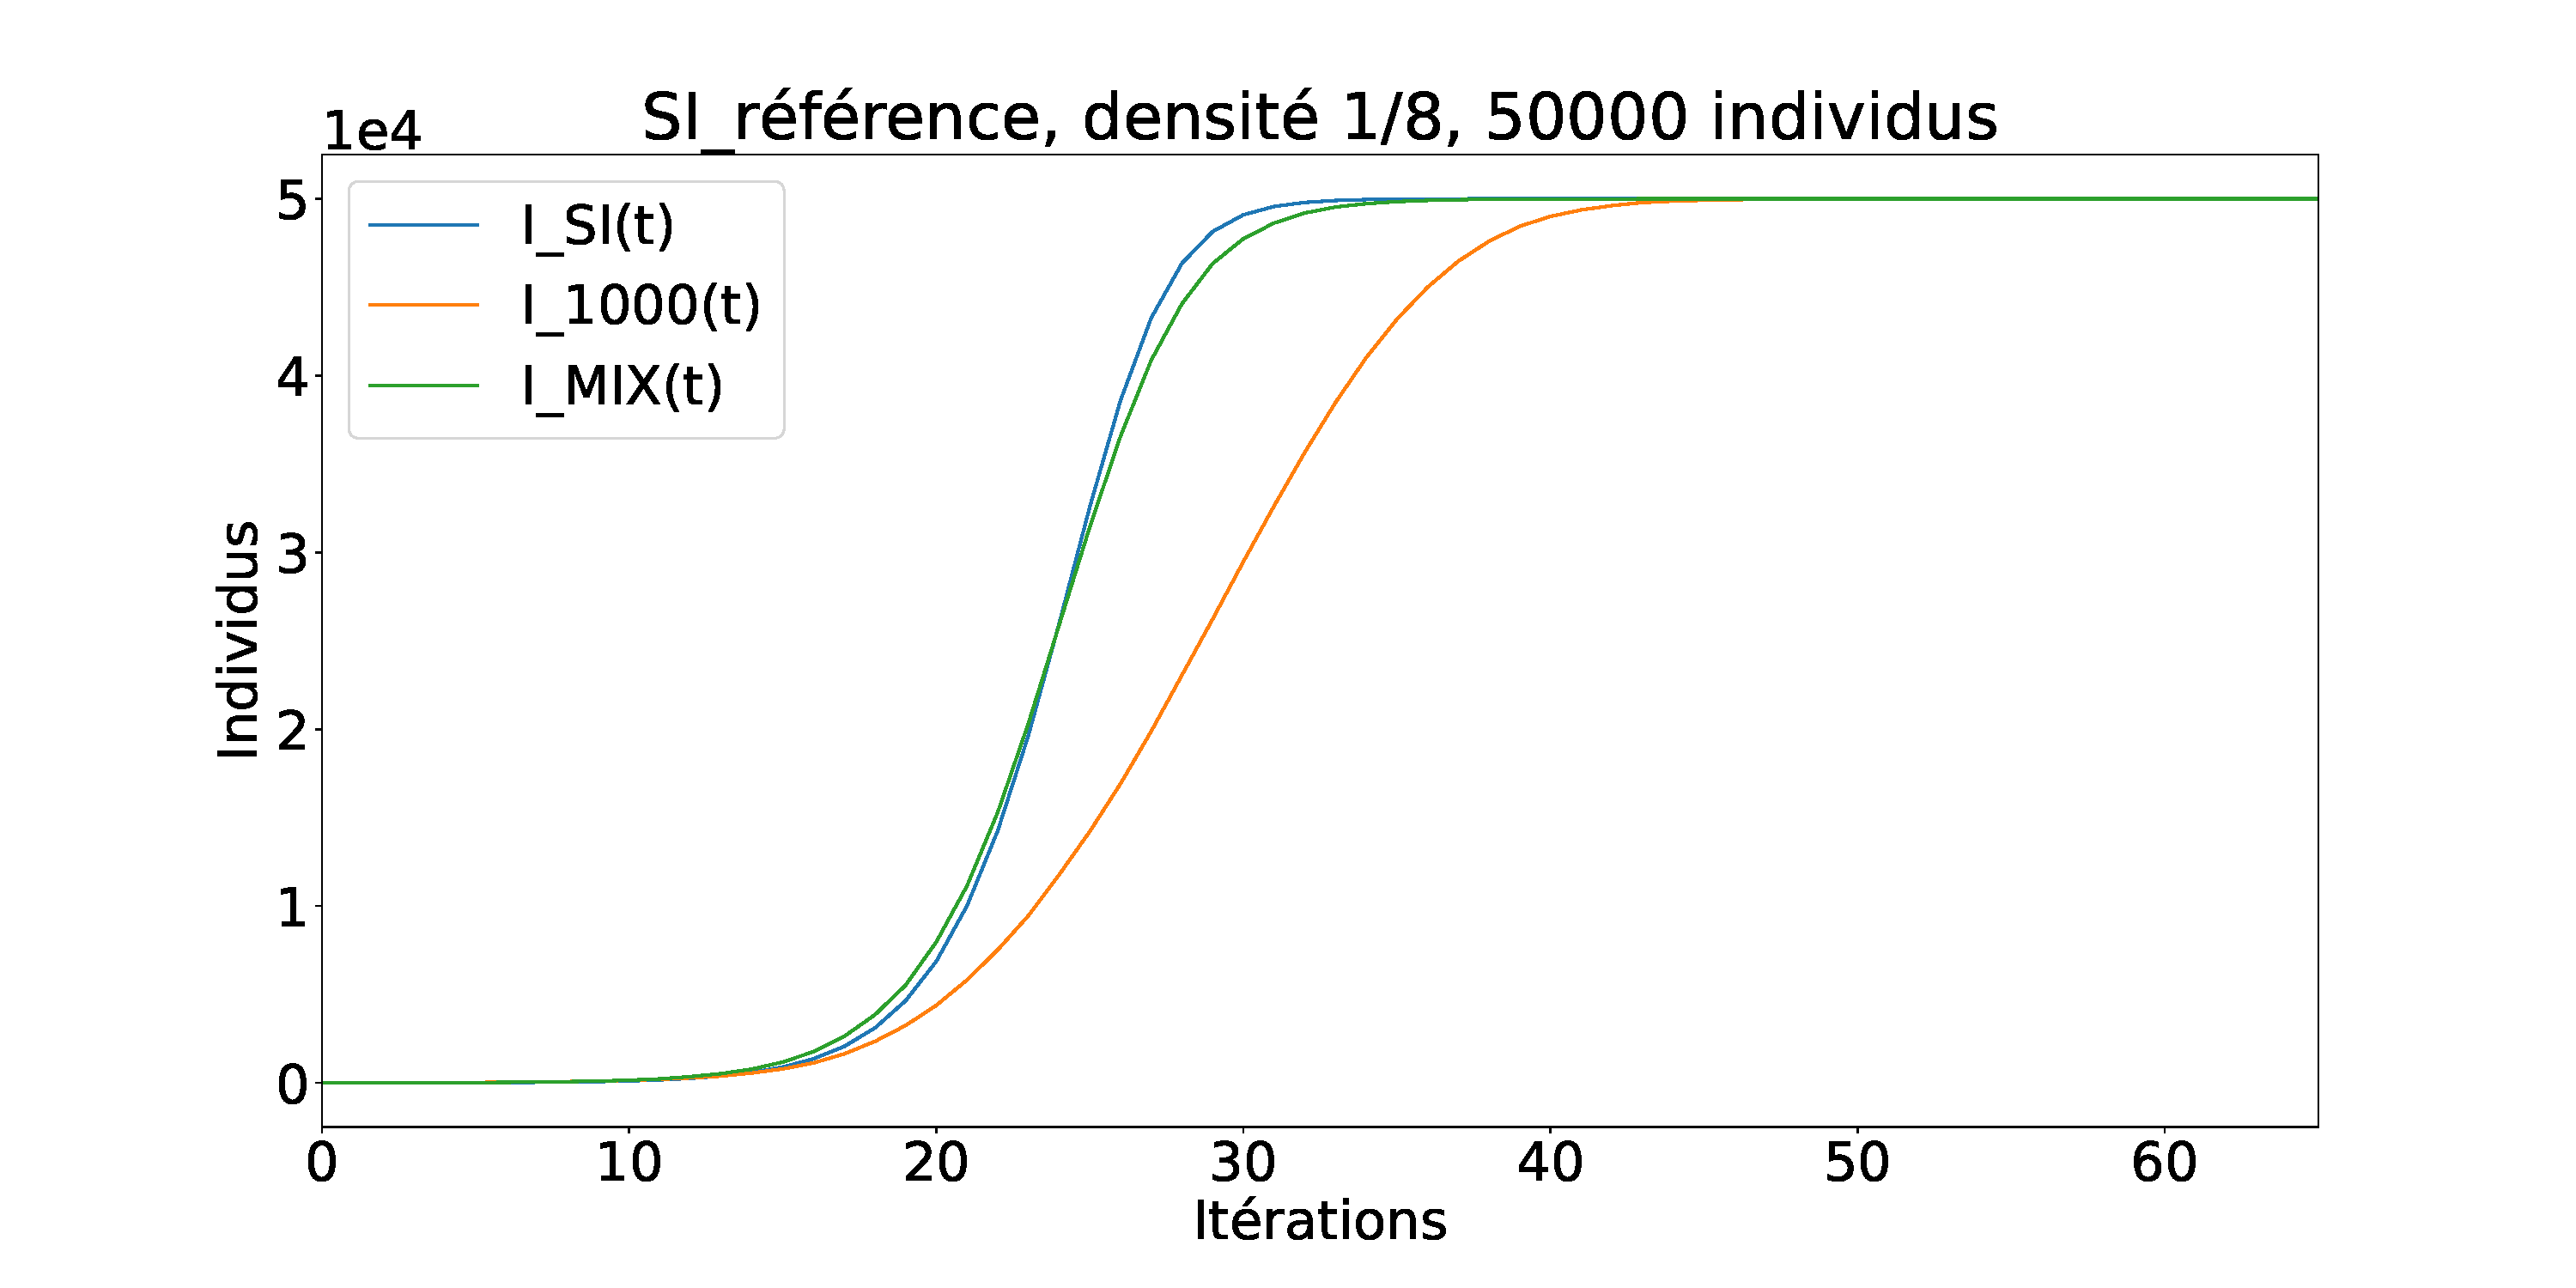
\includegraphics[width=0.5\textwidth]{Images/SI_ref_8_50k.pdf}
    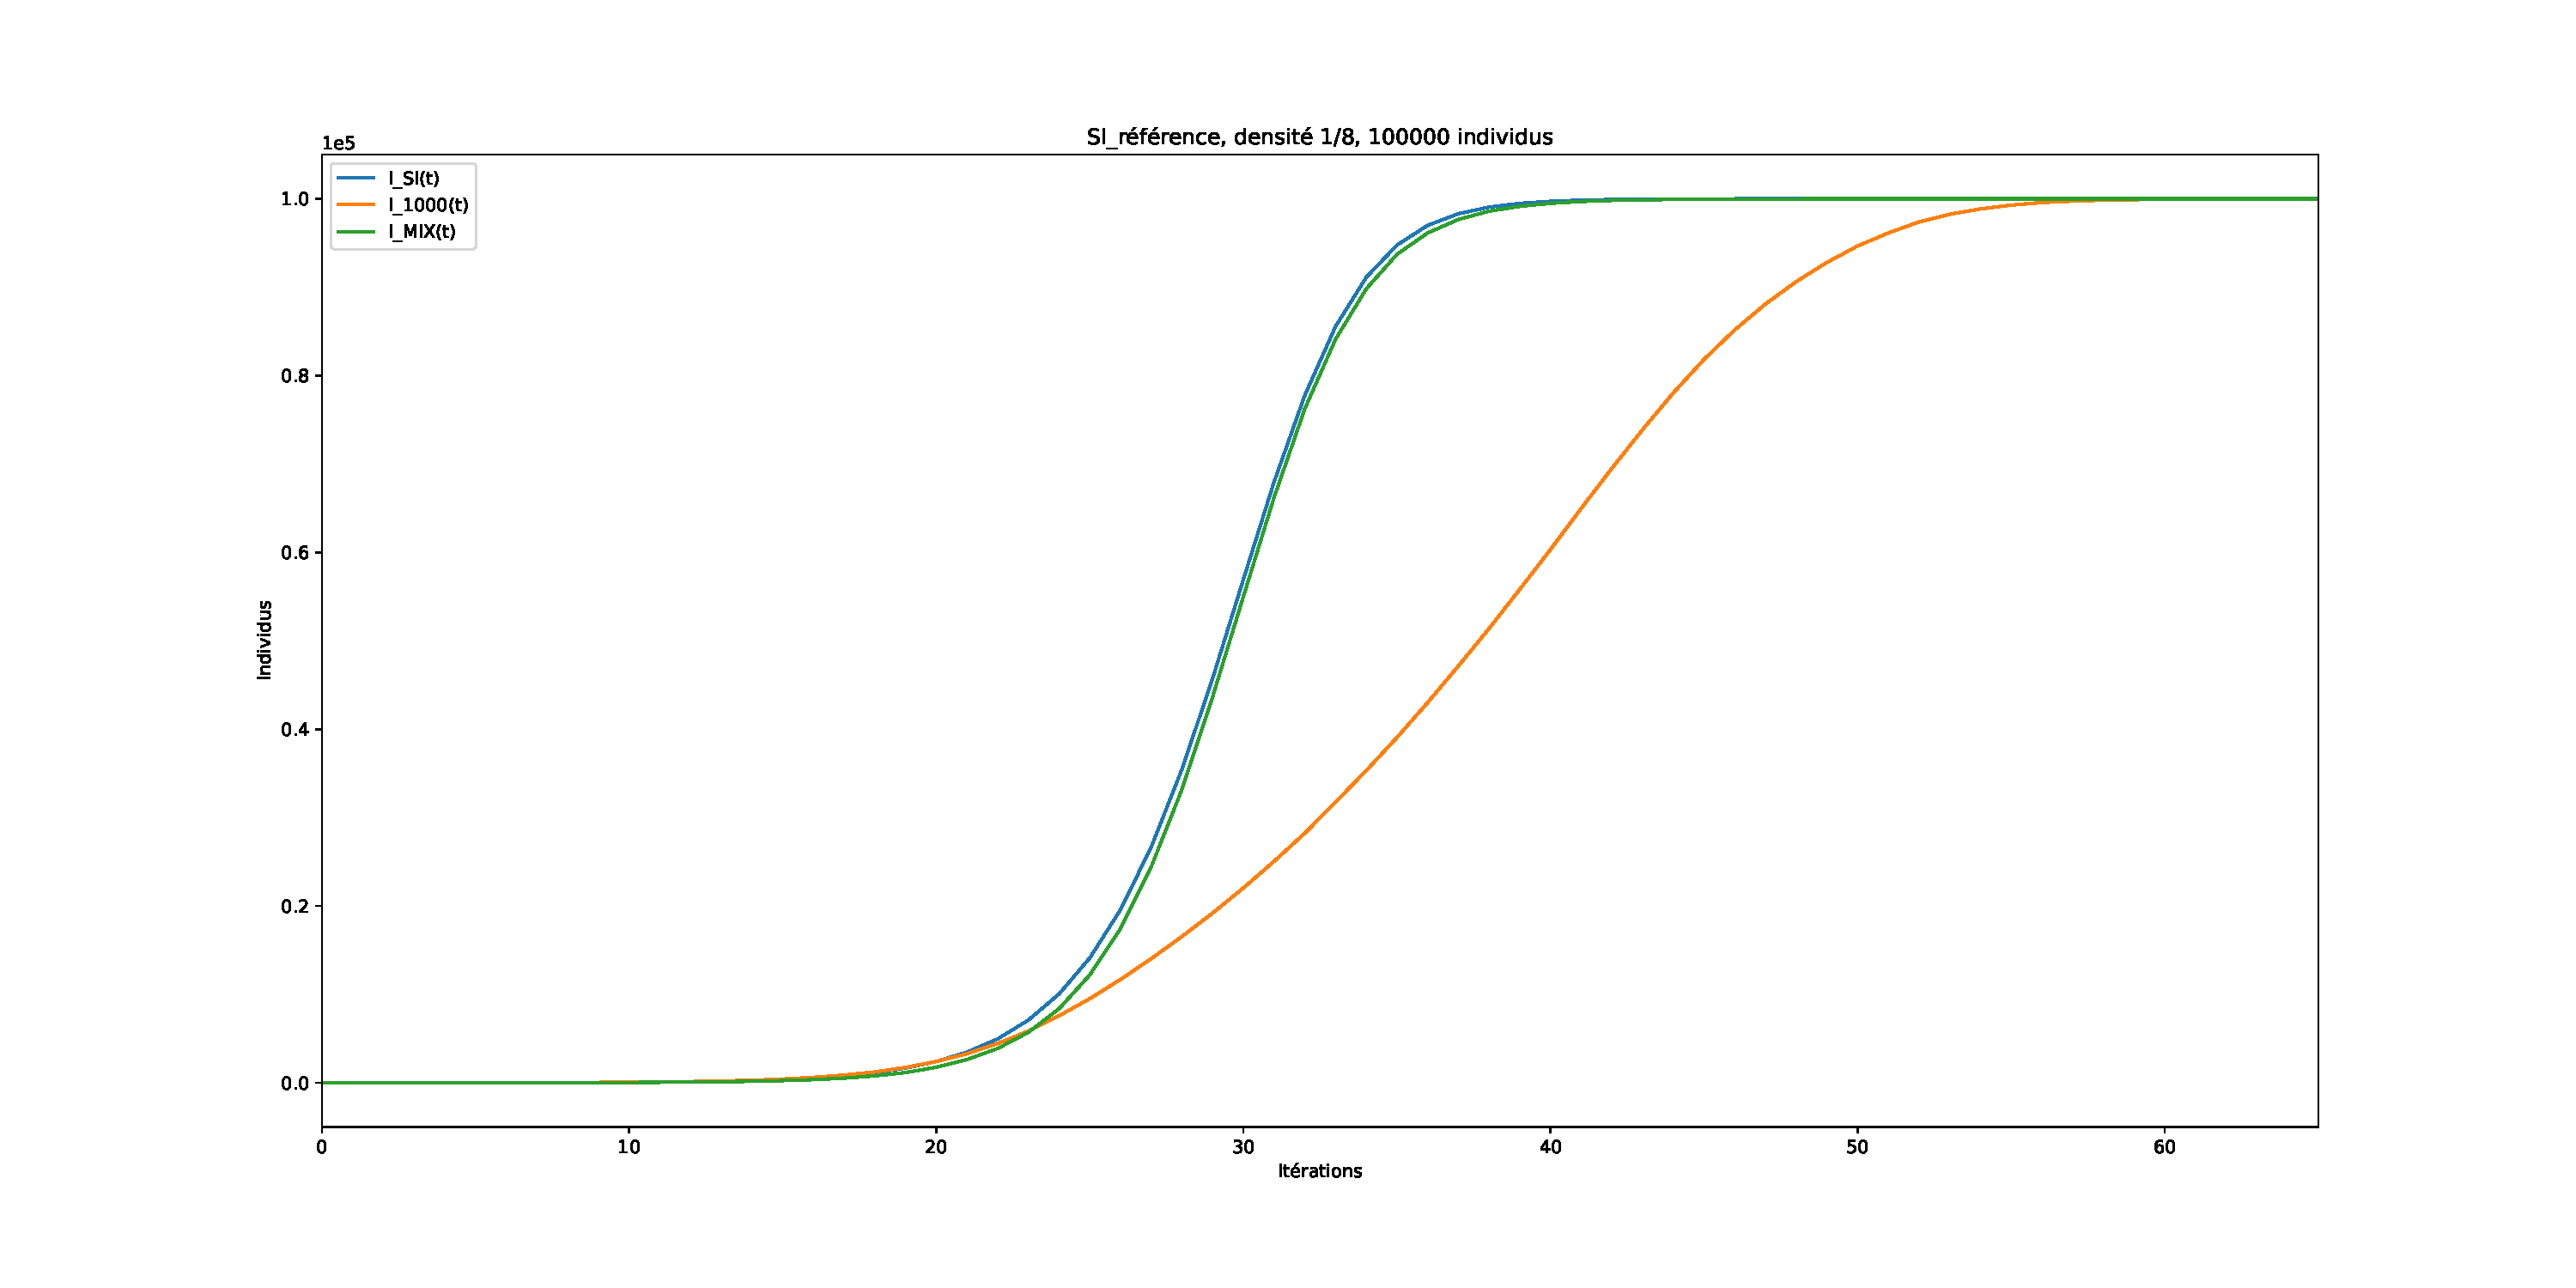
\includegraphics[width=0.5\textwidth]{Images/SI_ref_8_100k.pdf}
    \caption{Simulations de SI, densité 1/8}
\end{wrapfigure}

Les mêmes comportements sont observés pour les simulations en densité $\frac{1}{8}$. La qualité du mélange décroit avec l'augmentations de la taille des sytèmes et le mélange parfait est bon comparé au modèle mathématique SI. On remarque tout de même sur les trois simulations ($5000$, $20000$, $50000$) que les courbes de mélange parfait évoluent moins vite que le modèle SI. Ce comportement est logique car en diminuant la densité du système on réduit la probabilité d'entrer en contact avec d'autres individus et par conséquent de propager la contamination. Cette baisse de contact est en partie compensée par le fait que les individus ont (par la densité faible) la liberté de se déplacement plus aisément.\\

Un comportement intrigue sur la simulation à $20000$ individus. La courbe des $1000$ mouvements semble être décalée vers la droite sans pour autant qu'elle soit plus plate que le modèle SI. Ce comportement est du aux variations aléatoires sur les simulations. Lorsque la densité est faible le facteur chance croît ce qui a pour conséquence de déclencher des pandémies à des instants bien différents d'une simulation à l'autre. Ce phénomène est illustré et détaillé dans un chapitre ultérieur.

\newpage

\begin{wrapfigure}{r}{0.5\textwidth}
    \centering
    \captionsetup{justification=centering}
    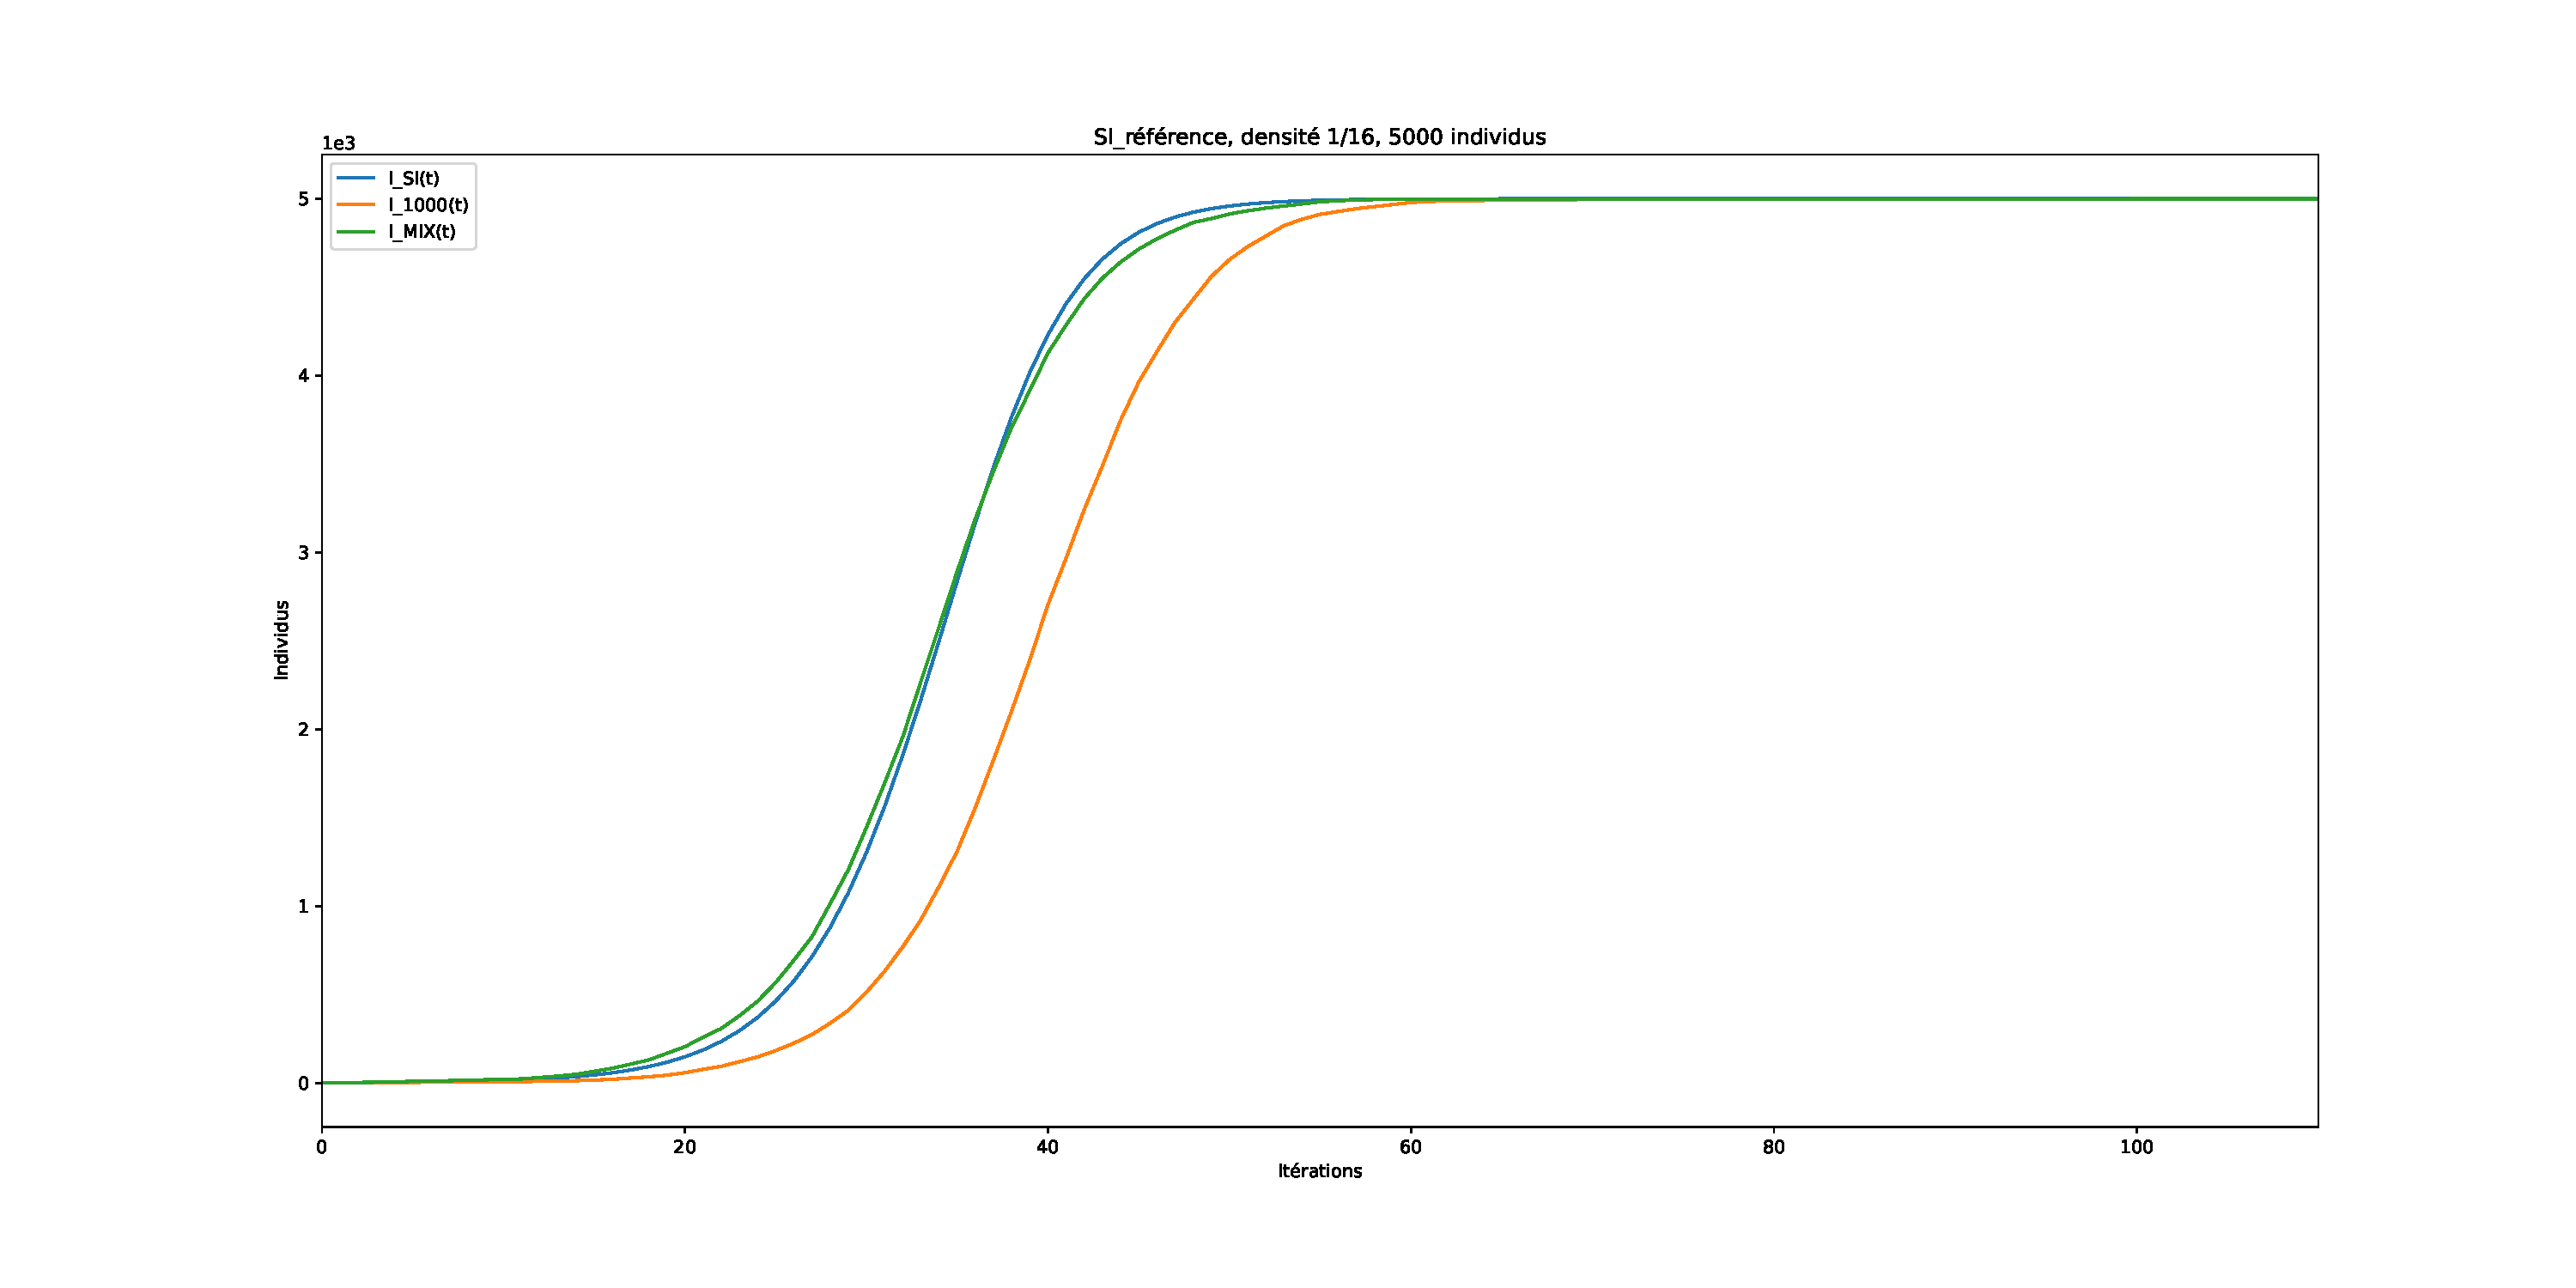
\includegraphics[width=0.5\textwidth]{Images/SI_ref_16_5k.pdf}
    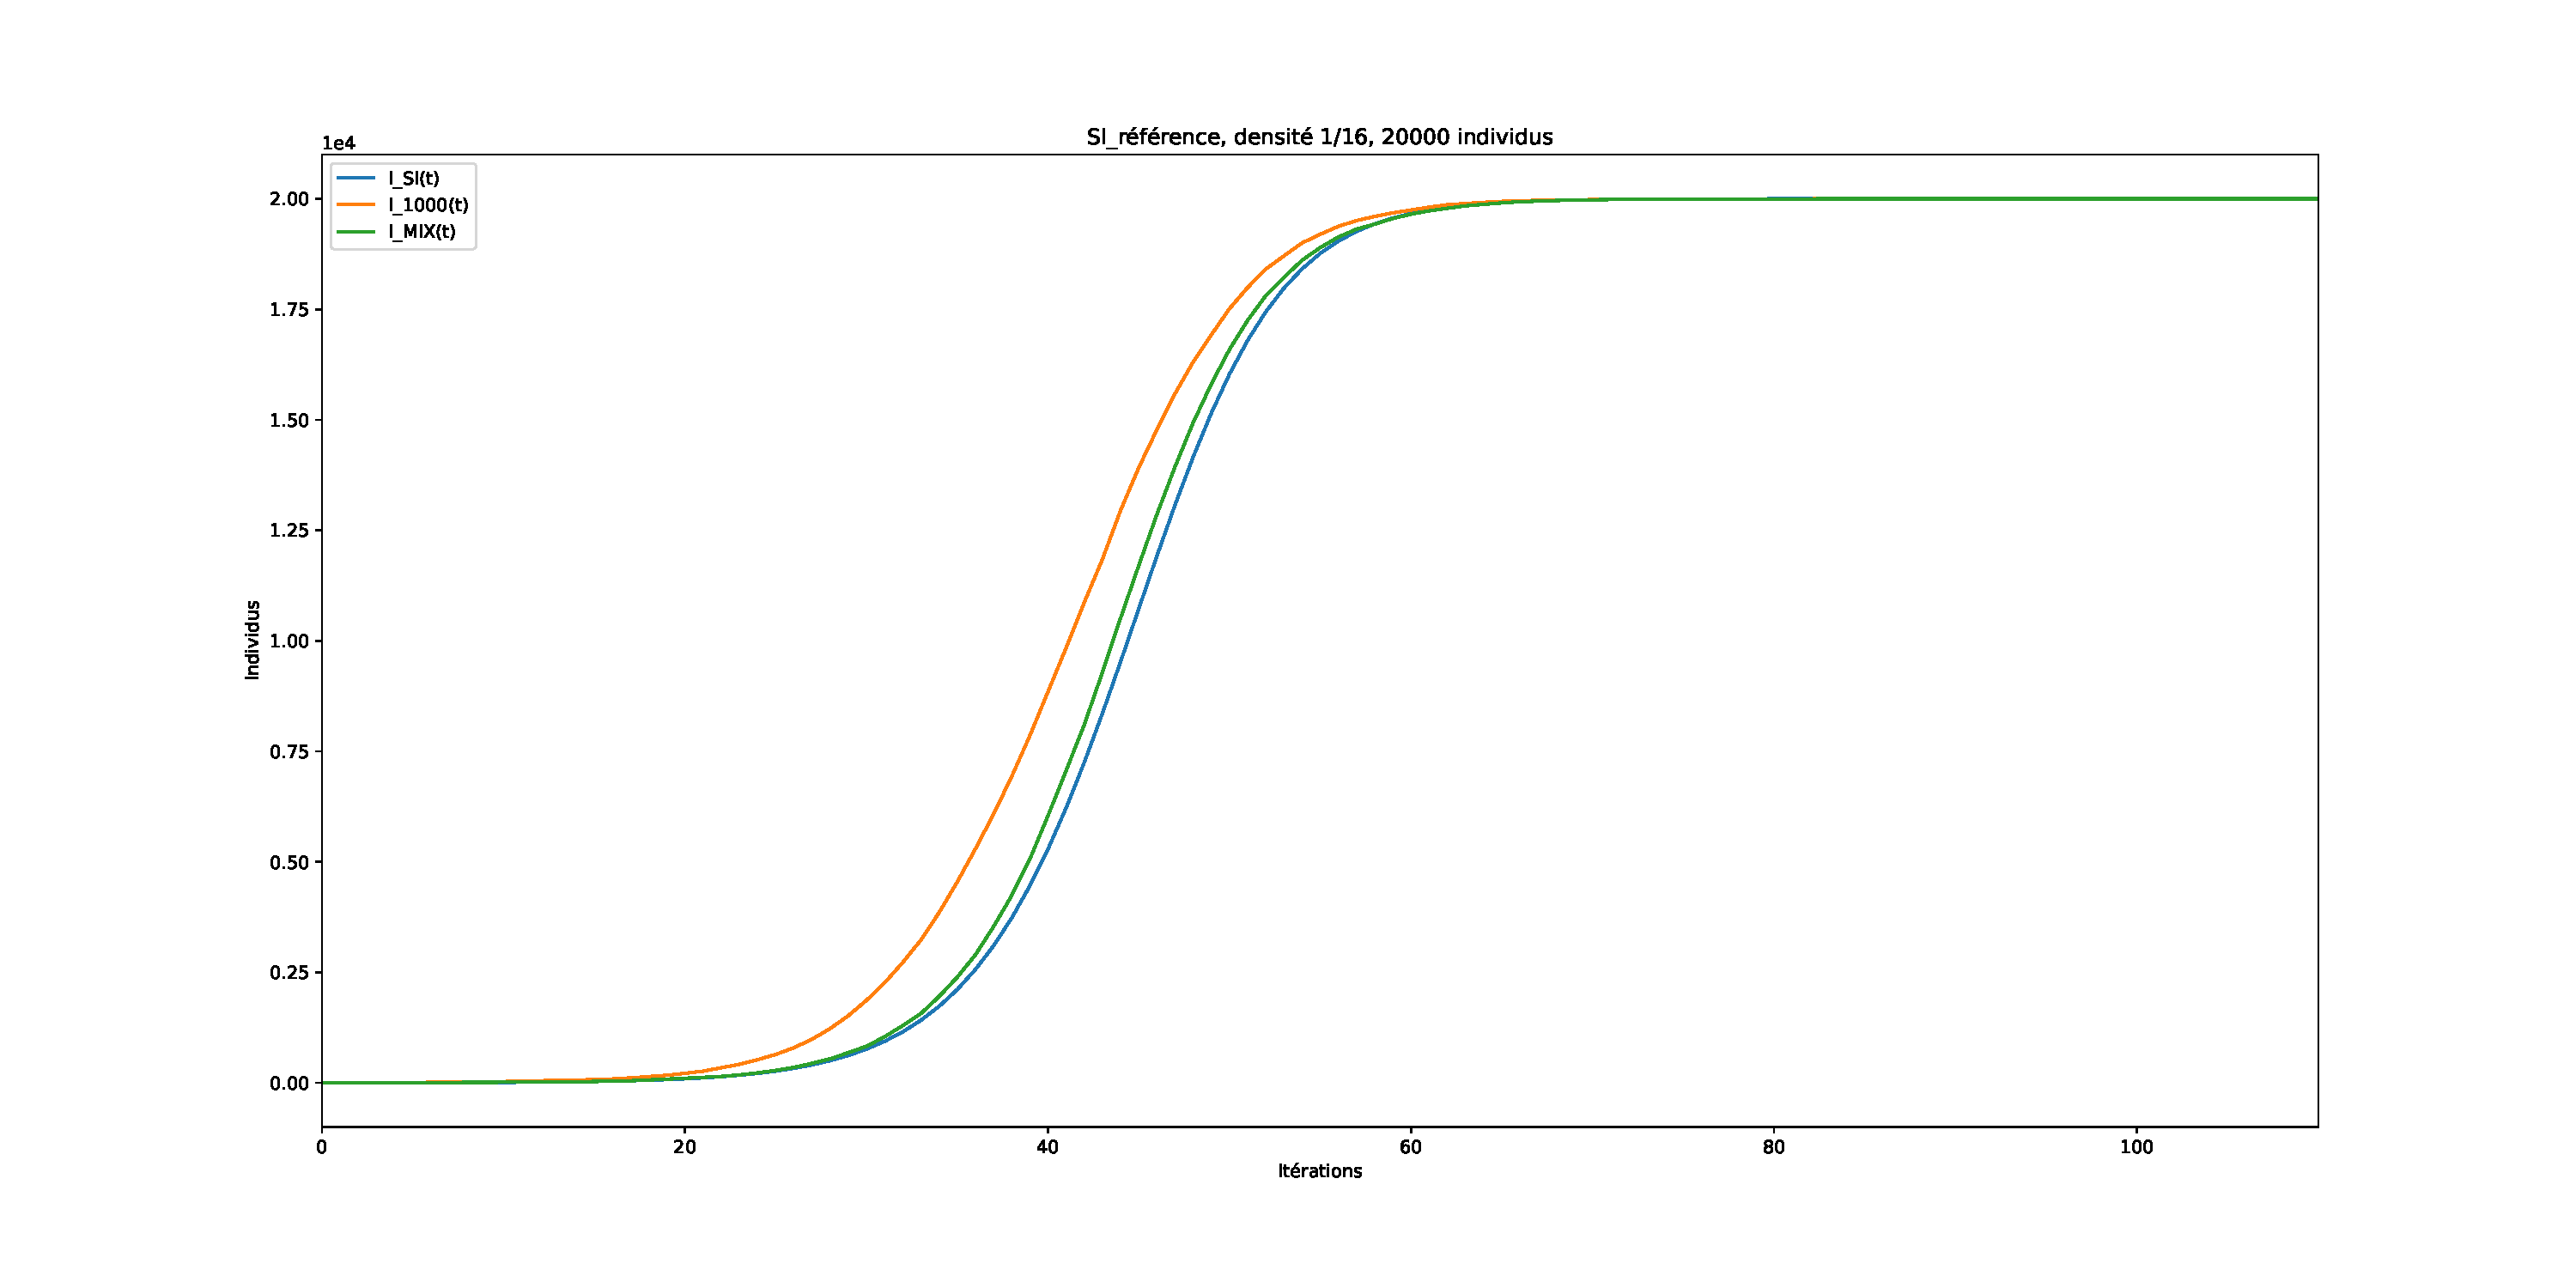
\includegraphics[width=0.5\textwidth]{Images/SI_ref_16_20k.pdf}
    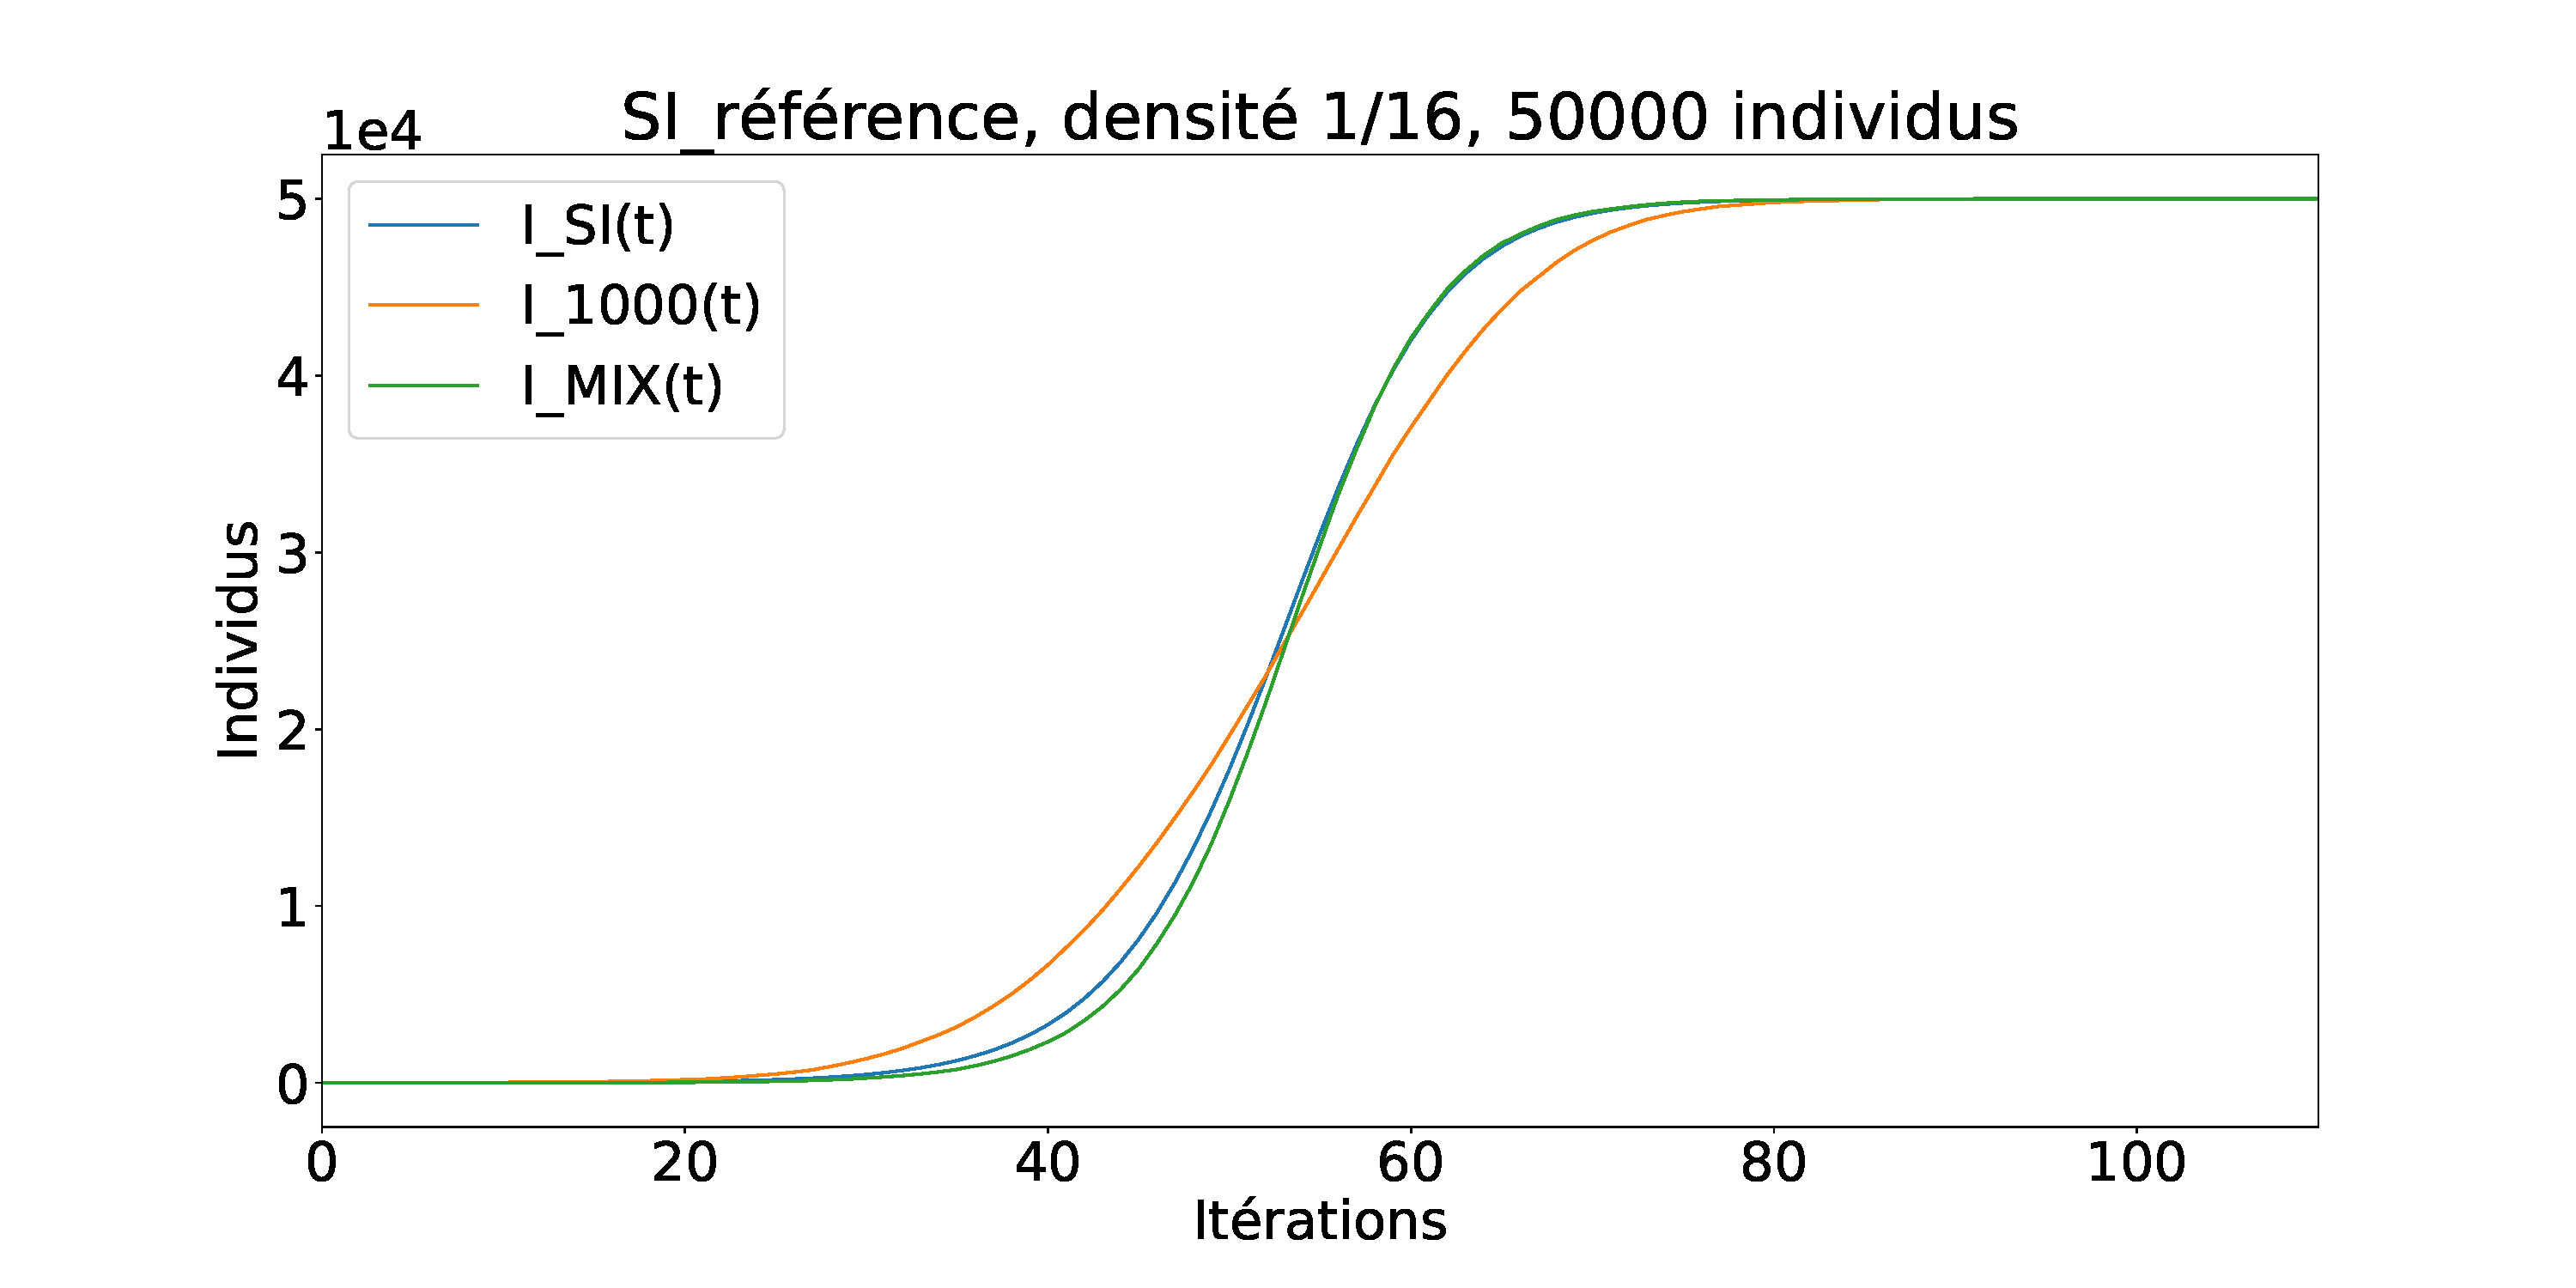
\includegraphics[width=0.5\textwidth]{Images/SI_ref_16_50k.pdf}
    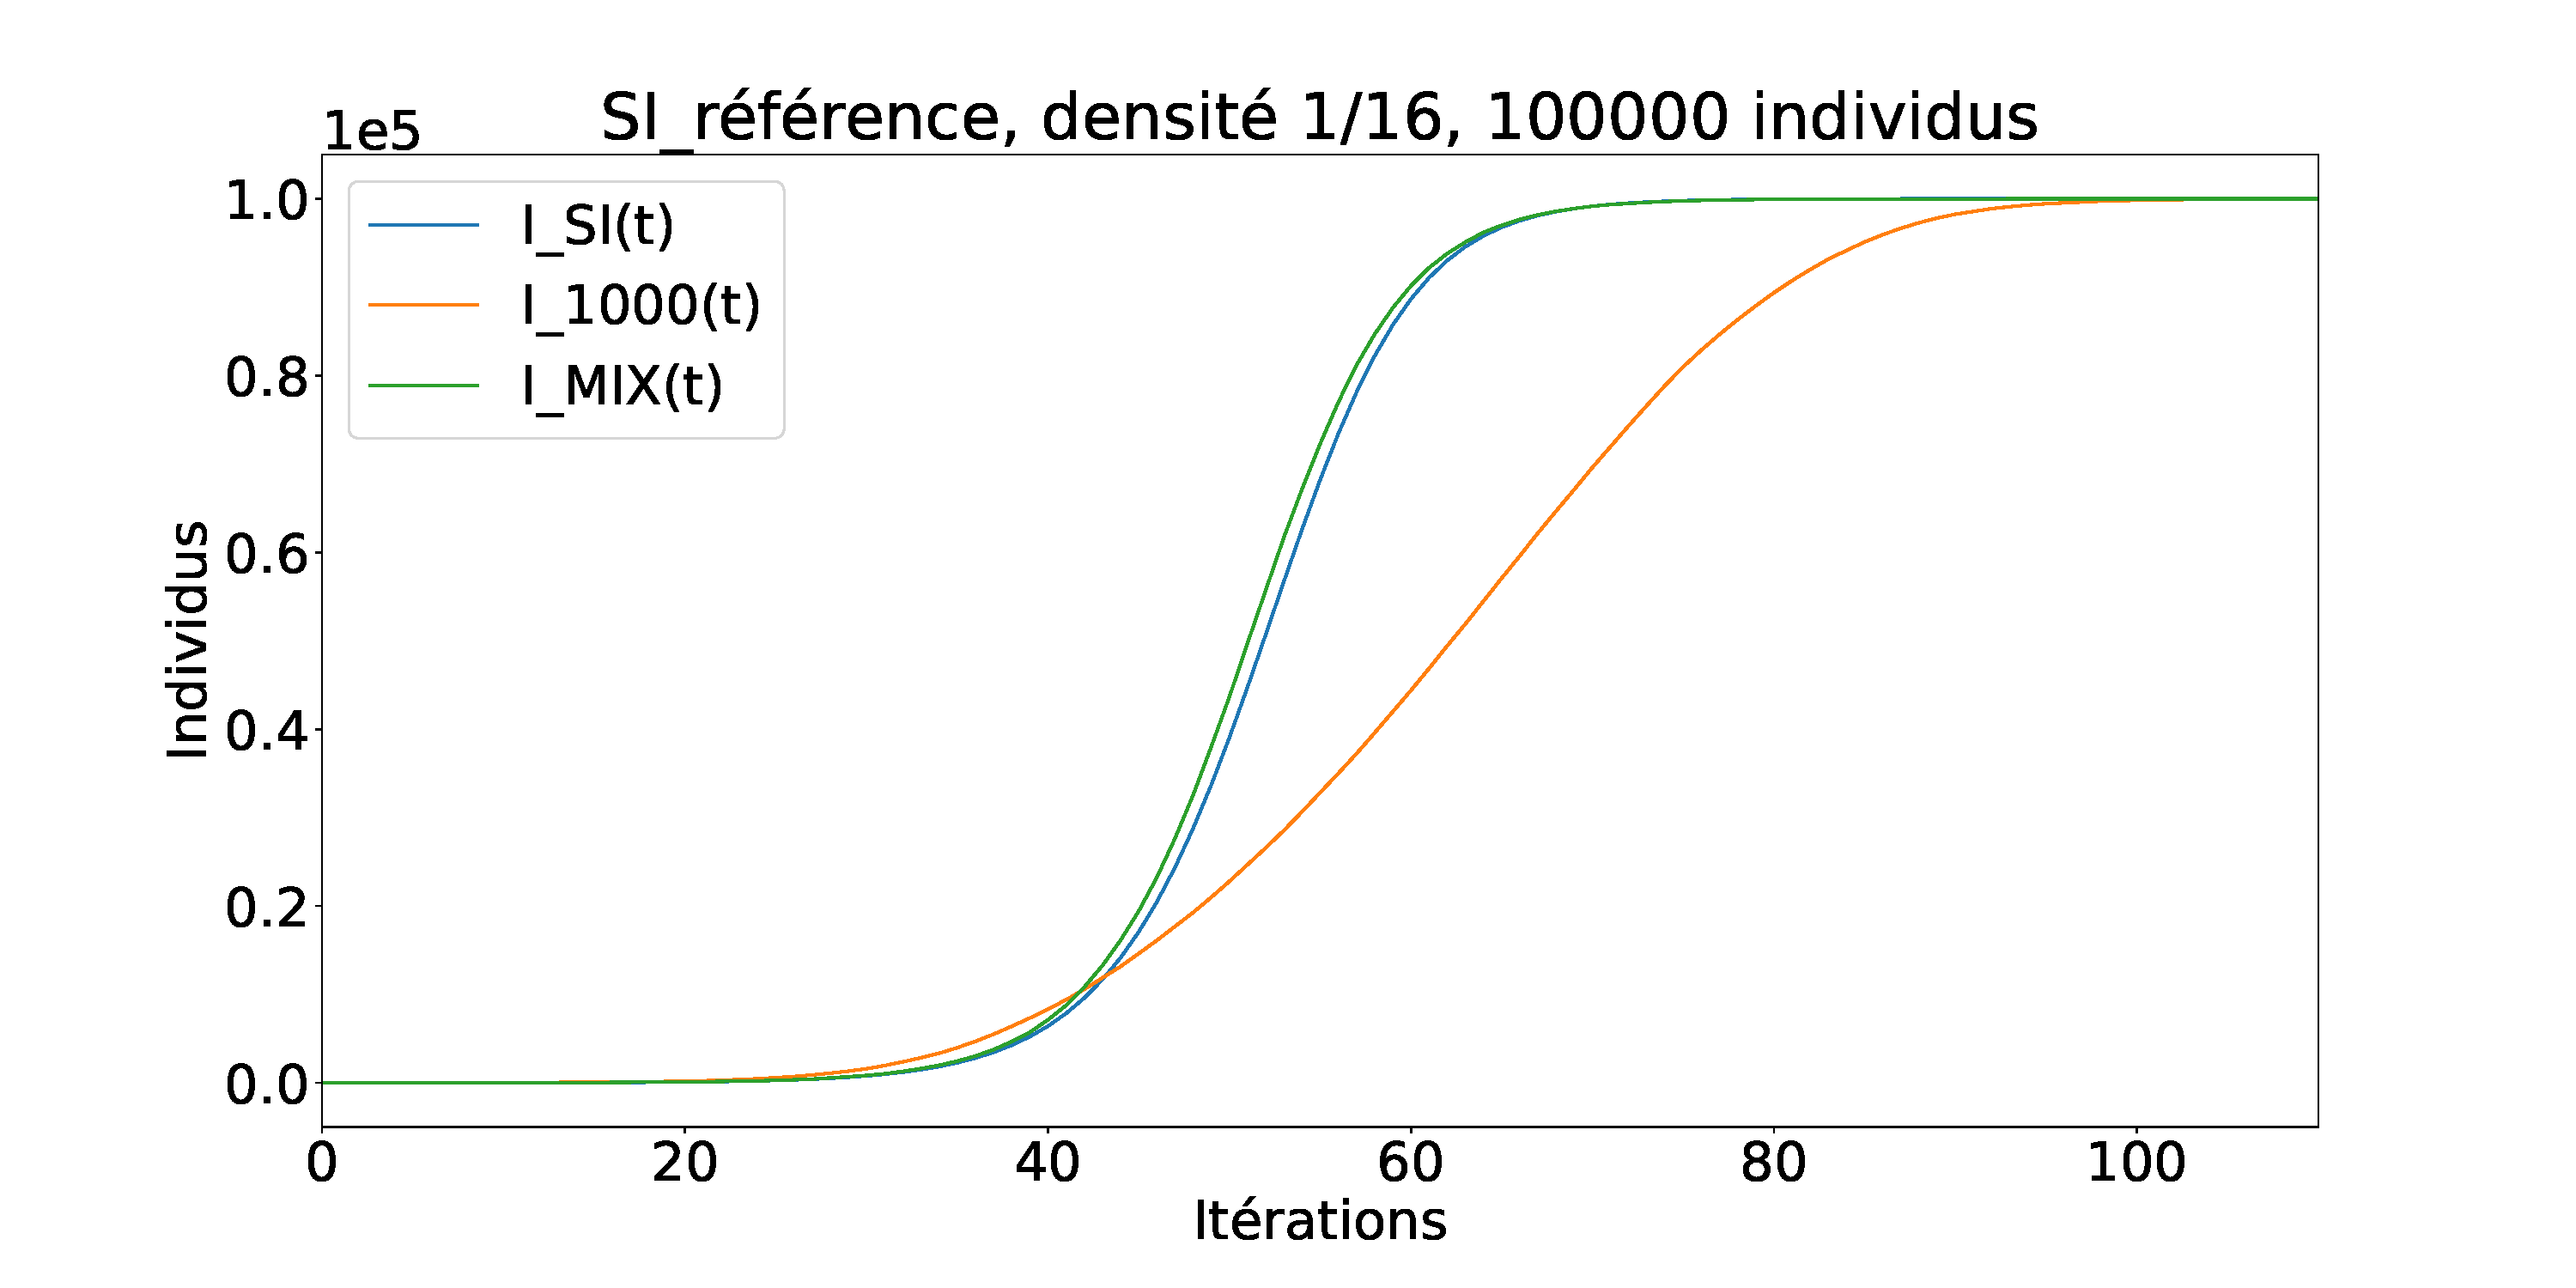
\includegraphics[width=0.5\textwidth]{Images/SI_ref_16_100k.pdf}
    \caption{Simulations de SI, densité 1/16}
\end{wrapfigure}

Finalement les simulations en densité $\frac{1}{16}$ donnent aussi de bons résultats. Les mêmes comportements sont observés sur ces simulations mais la simulation à $50000$ individus montre un nouveau comportement pas encore observé sur les autres simulations. L'effet ici est assez faible mais on peut distinguer que la courbe du mélange parfait croît plus rapidement que le modèle mathématique SI. Nous avons donc une simulation qui évolue plus rapidement que le modèle SI. Cet effet n'est pas du au fait que le modèle implémenté est plus rapide mais uniquement au temps qu'il a fallu pour la pandémie se déclare. En effet le modèle SI n'a aucun temps de latence et commence donc à l'itération $0$. Les mesures prisent sur SI souffrent peu de de phénomène contrairement à certaines simulations par la suite. \\

Tout comme pour les simulations en densité $\frac{1}{8}$, nous pouvons observer de fortes variations sur les moments de déclenchement de pandémies. Sur la première simulations ($5000$ individus), la courbe des $1000$ mouvement est retardée. Sur les trois autres c'est l'effet inverse. Ce comportement est illustré et mesuré plus loin.

\newpage

\section{Analyses}

\subsection{Mean Absolute Error}

L'objectif du chapitre précédent est de prouver la validité du modèle implémenté en comparant les résultats avec des résultats bien connus du modèle SI. Le mean absolute error est un calcul d'erreur qui consiste à sommer toutes les différences entre les courbes et à calculer la moyenne de ces différences. Les résultats sont normalisés c'est-à-dire que nous divisons le MAE (mean absolute error) par le nombre d'individus. Ceci permet de comparer les résultats pour des simulations de taille différente.\\

Les mesures qui suivent comparent le modèle mathématique SI avec les simulations au mélange parfait.

\begin{table}[H]
\centering
\captionsetup{justification=centering}
\caption[Mean Aboslute Error Normalized : SI]{Mean Aboslute Error Normalized : modèle SI, mélange parfait \label{tab:grid}}
\begin{tabular}{@{\extracolsep{\fill} } c|| c| c| c| c|}
 & 5000 & 20000 & 50000 & 100000\\ 
\midrule
\midrule
1/2 & $6.2\mathrm{e}{-4}$ & $6.4\mathrm{e}{-4}$ & $6.4\mathrm{e}{-4}$ & $7.3\mathrm{e}{-4}$\\
\midrule
1/4 & $9.0\mathrm{e}{-4}$ & $7.9\mathrm{e}{-4}$ & $7.7\mathrm{e}{-4}$ & $9.5\mathrm{e}{-4}$\\
\midrule
1/8 & $3.2\mathrm{e}{-3}$ & $1.9\mathrm{e}{-3}$ & $2.8\mathrm{e}{-3}$ & $2.0\mathrm{e}{-3}$\\
\midrule
1/16 & $4.2\mathrm{e}{-3}$ & $4.6\mathrm{e}{-3}$ & $4.2\mathrm{e}{-3}$ & $4.6\mathrm{e}{-3}$\\
\bottomrule
\end{tabular}
\end{table}

Les résultats suivent les observations du chapitre précédent. Tout d'abord nous remarquons que l'erreur est constante pour une densité fixée, c'est-à-dire que l'erreur ne croit pas avec la taille du système. Pour ces analyses, la magnétude des erreur ne sont pas importantes, ce qui nous intéresse est de comparer les valeurs les unes avec les autres. \\

Le deuxième résultat intéressant est que l'erreur augmente lorsque nous diminuons la densité du système. Ce comportement suit les observations des figures au chapitre précédent. L'erreur est due au temps de latence dont souffrent les systèmes moins denses. Une section ultérieur est dédié aux latences des grands systèmes.


\subsection{Moyenne de voisinage}

Les courbes des simulations ont montré des comportements peu intuitifs, surtout pour les systèmes peu denses. Cette section analyse le nombre de voisins moyens par individu pour ces simulations afin de déterminer si les résultats sont influencés par des mécaniques cachées derrière les mouvements des individus. Il s'agit ici de comparer la densité du voisinage de simulations au mélange parfait avec des simulations aux $1000$ mouvements. L'hypothèse derrière cette recherche est de déterminer si le déplacement des individus implique d'avantages de contactes que la méthode du mélange parfait.\\

Nous nous intéressons aux simulations de faible densité car ce sont sur ces simulations que les comportements non intuitifs apparaissent. Les mesures sont prises sur des systèmes de densité $\frac{1}{8}$ ainsi que $\frac{1}{16}$ avec $5000$ individus. Les simulations les plus petites ont été choisie pour des questions de temps de calcul mais aussi du fait que les micro mécaniques que nous essayons de détecter ne sont pas sensibles à la taille du système car c'est une analyse local à chaque individu.\\

Les mesures pour le système en densité $\frac{1}{8}$ ont été effectué sur $65$ itérations puis moyenné. Les mesures pour le système de densité $\frac{1}{16}$ ont été effectué sur $110$ itérations puis moyenné. Ces itérations ont été choisies par rapport aux bornes des figures de la section "Résultats".

\begin{table}[H]
\centering
\captionsetup{justification=centering}
\caption[Voisinage moyen : SI]{Voisinage moyen : modèle SI, mélange parfait, 1000 mouvements \label{tab:grid}}
\begin{tabular}{@{\extracolsep{\fill} } c|| c| c|}
 & 1000 & perfect\_mix\\ 
\midrule
\midrule
1/8 & $0.498$ & $0.494$\\
\midrule
1/16 & $0.248$ & $0.250$\\
\bottomrule
\end{tabular}
\end{table}

Les résultats montrent que le mode de mouvements n'influence pas la densité du voisinage, car conséquent les phénomènes observés dans les figures ne sont pas causés par la densité du voisinage. De plus les résultats nous réconforte dans le fonctionnement du modèle implémenté. En effet les valeurs sont attendues, pour une densité de $\frac{1}{8}$ nous nous attendions à avoir en moyenne $4\times \frac{1}{8} = 0.5$ et pour une densité de $\frac{1}{16}$ nous nous attendions à une moyenne de $4\times \frac{1}{16} = 0.25$.

\subsection{Variations aléatoires}

Une autre hypothèse qui pourrait expliquer les comportements observés est que les simulations ne soient pas déterministe, c'est-à-dire qu'un facteur aléatoire détermine à quel instant la pandémie se déclare. Cela signifie que deux simulations aux paramètres identiques produisent deux résultats différents.\\

L'objectif de cette section est de mesures cette variation sur des simulations à faible densité. Les densités étudiées sont $\frac{1}{8}$ et $\frac{1}{16}$ avec une population de $20000$ individus. Pour chaque densité, les deux modes de déplacements sont étudiés et ceci sur un total de $20$ simulations. Nous représentons donc $20$ simulations avec des paramètres identiques et observons les différences.

\newpage

\begin{wrapfigure}{r}{0.5\textwidth}
    \centering
    \captionsetup{justification=centering}
    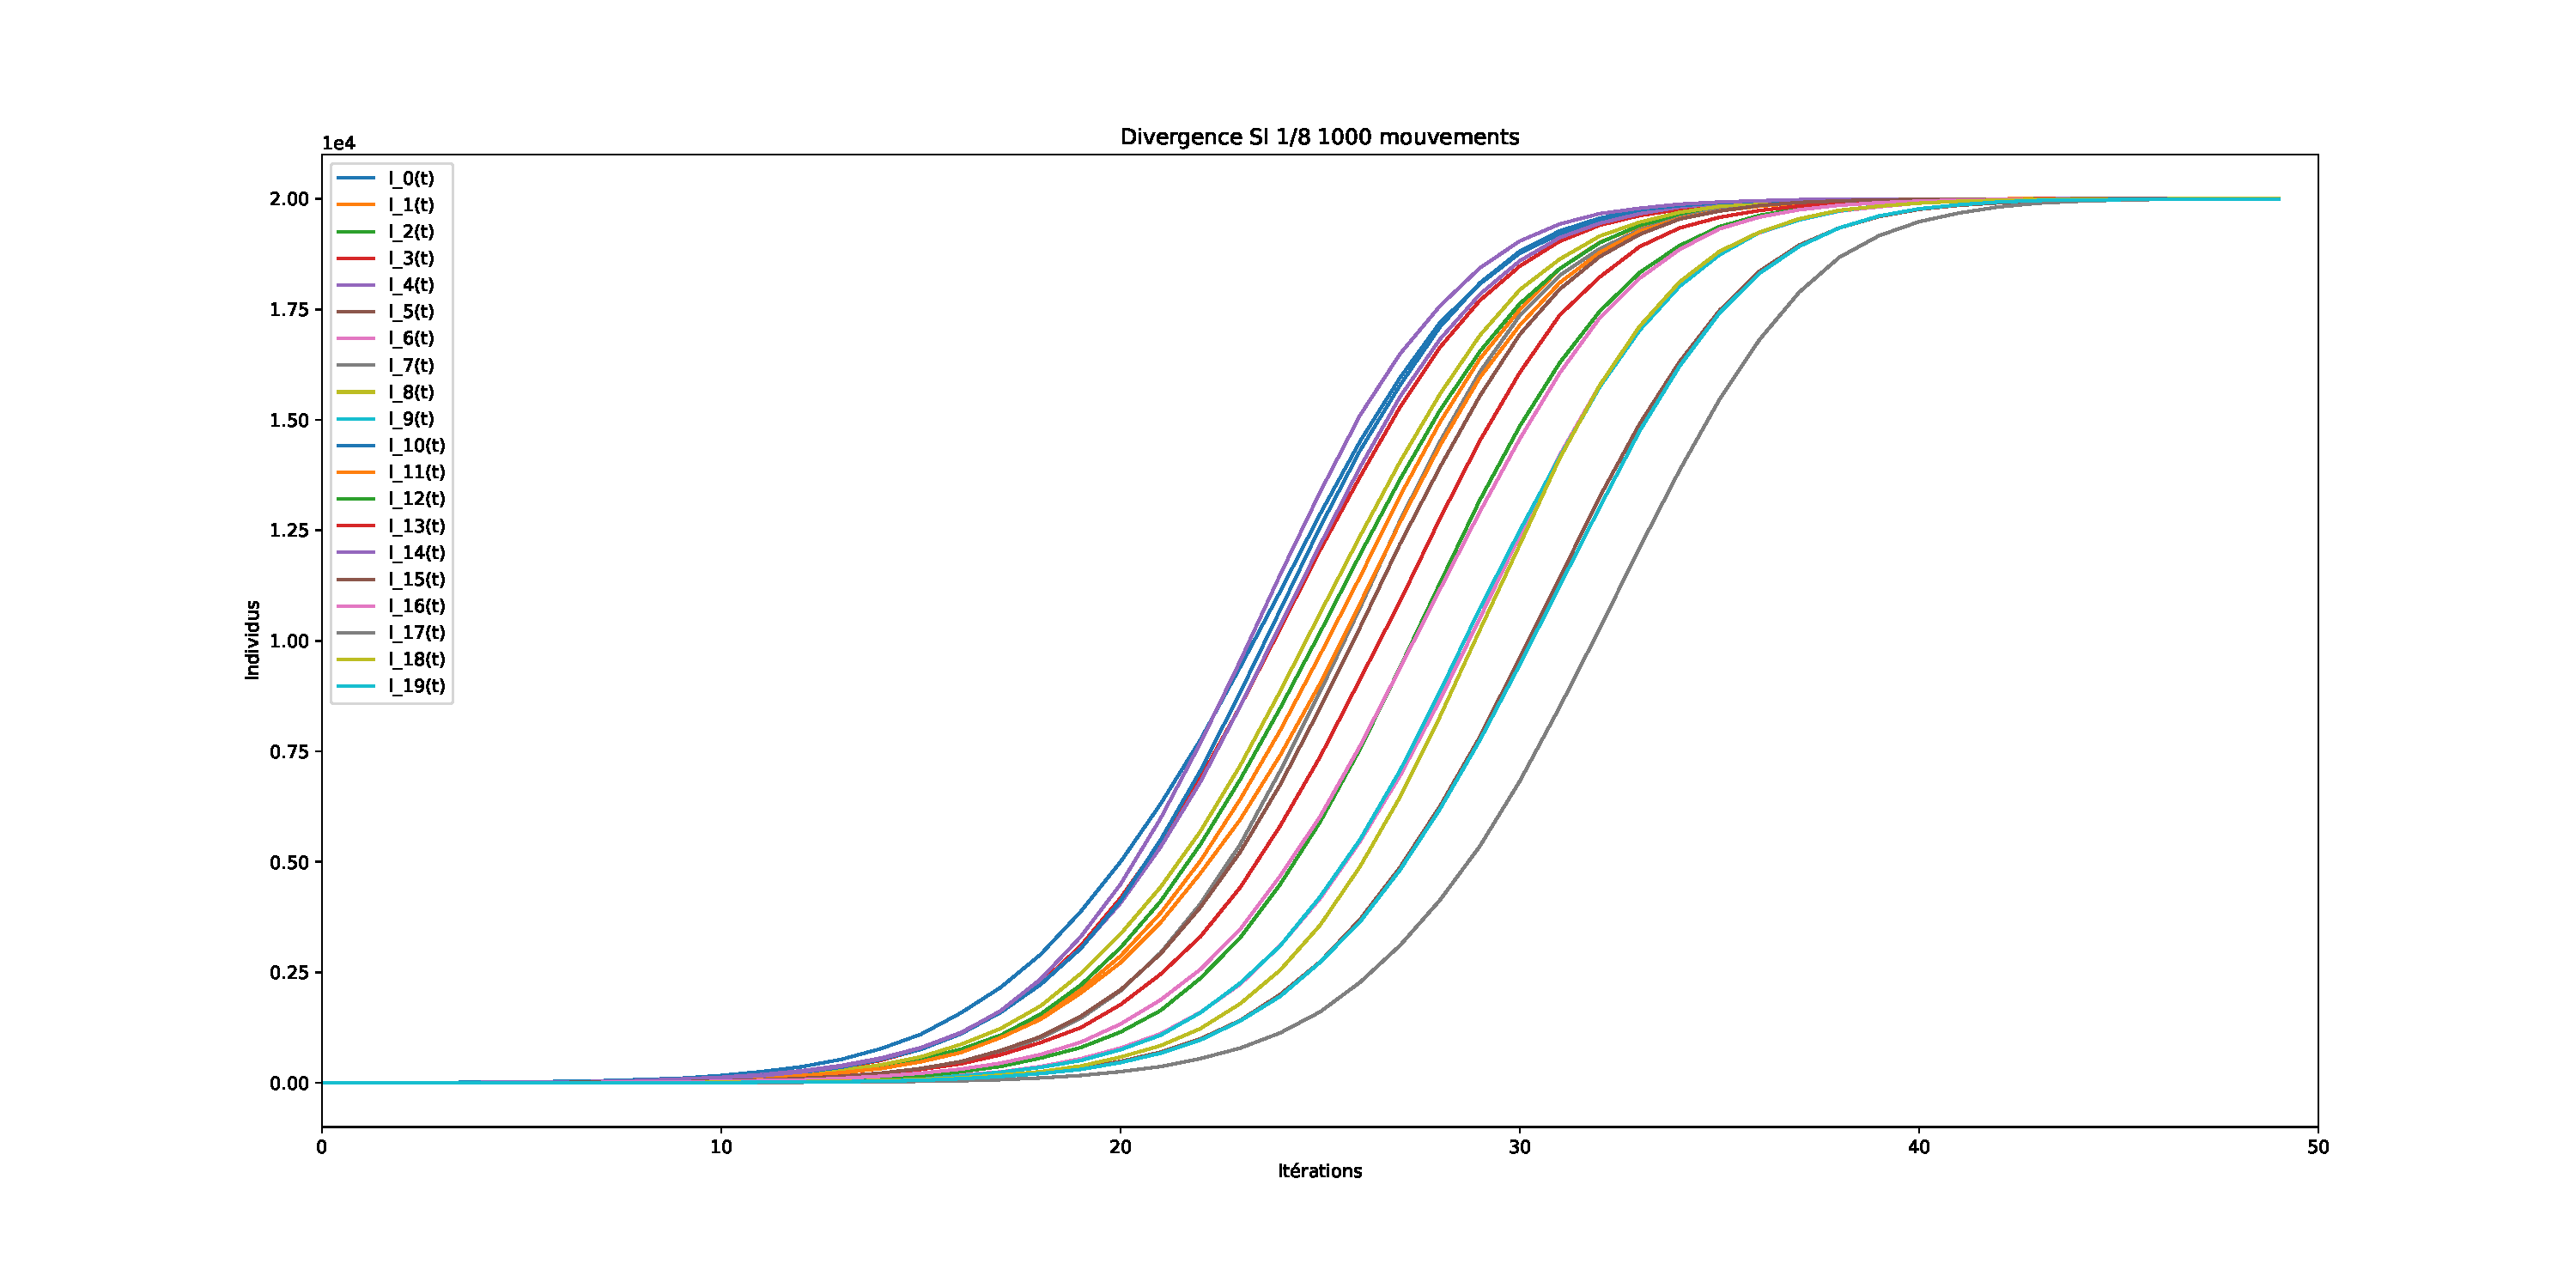
\includegraphics[width=0.5\textwidth]{Images/SI_divergence_8_1000.pdf}
    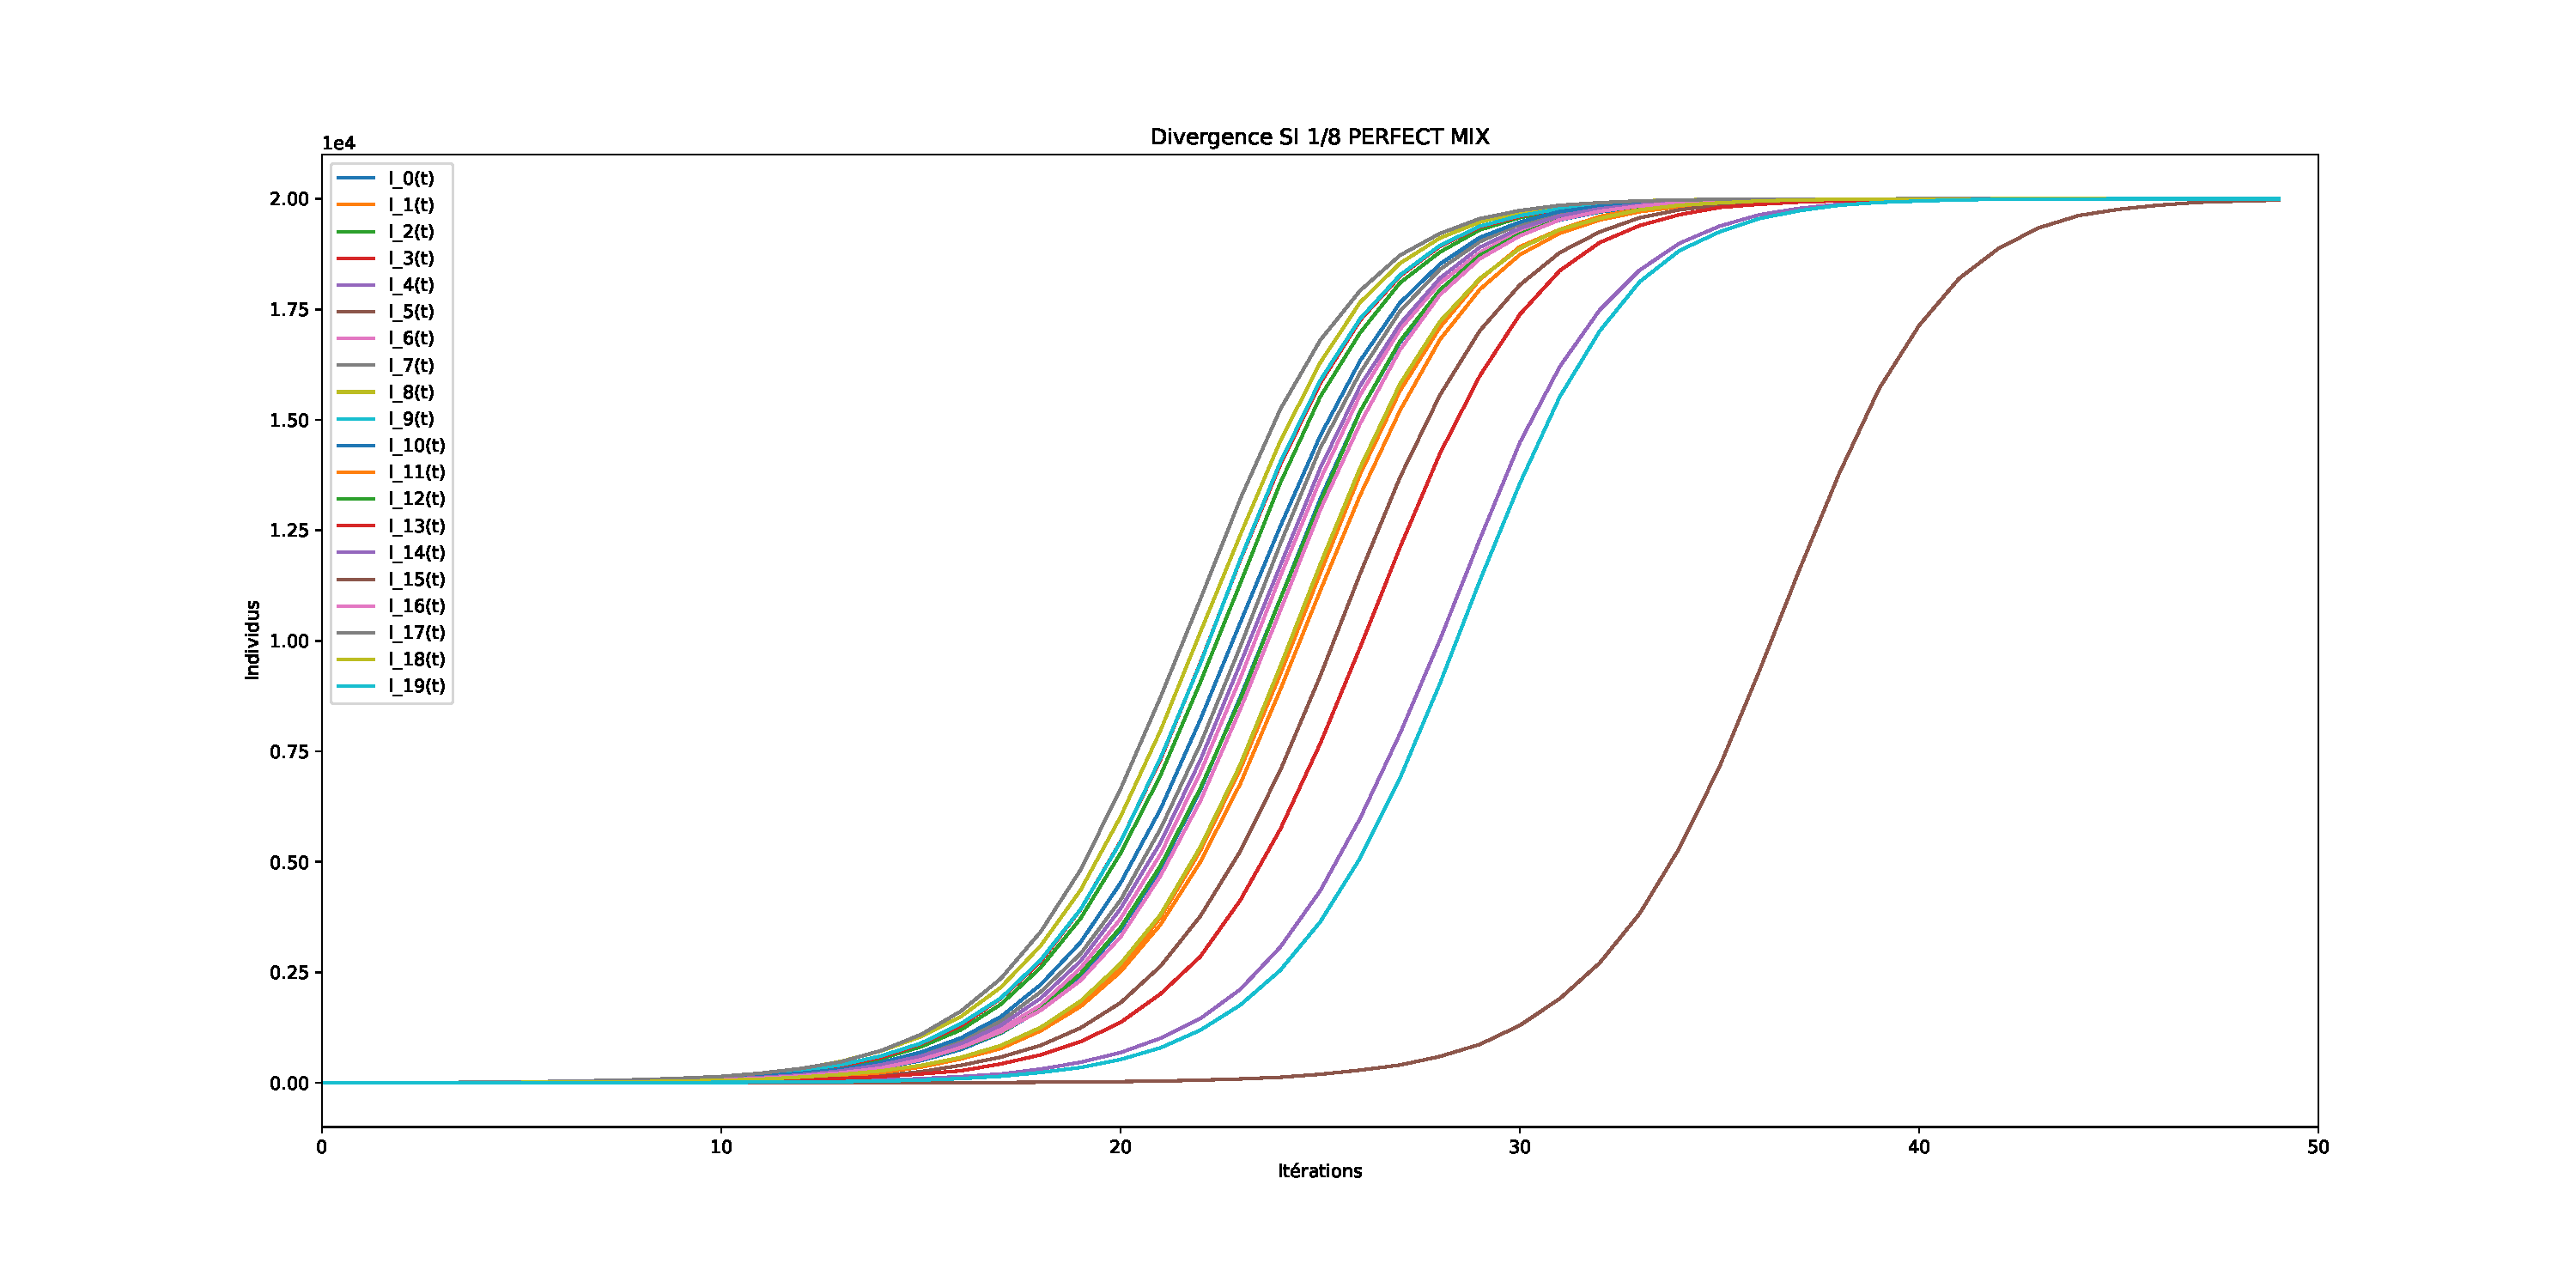
\includegraphics[width=0.5\textwidth]{Images/SI_divergence_8_mix.pdf}
    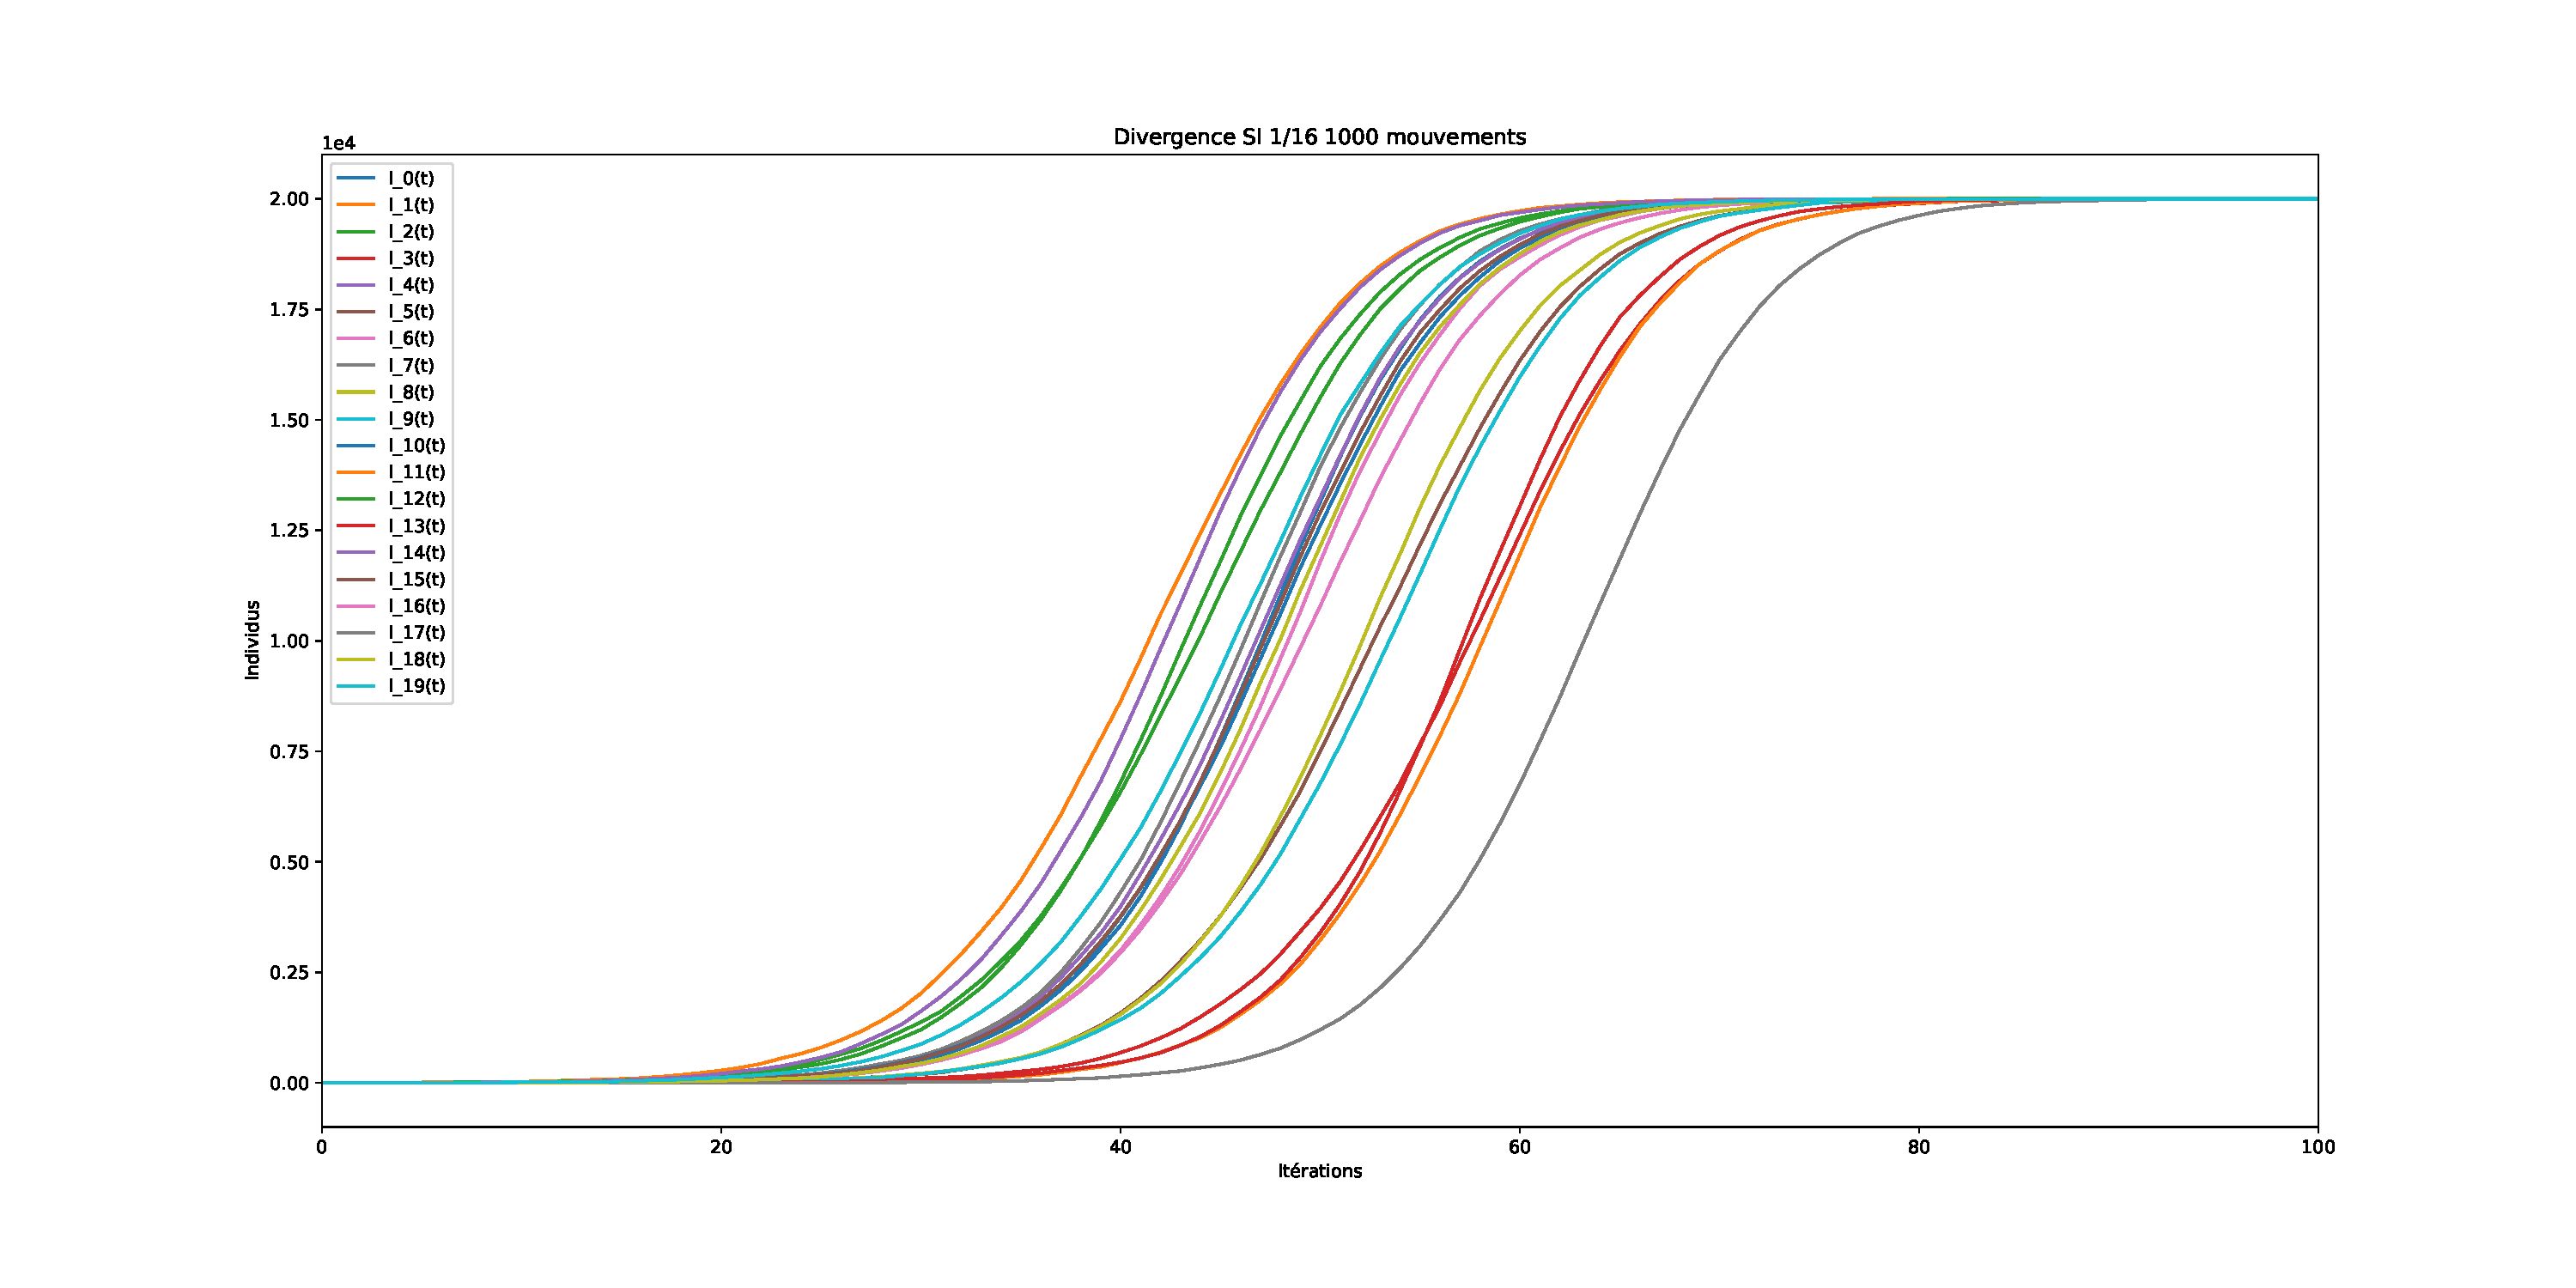
\includegraphics[width=0.5\textwidth]{Images/SI_divergence_16_1000.pdf}
    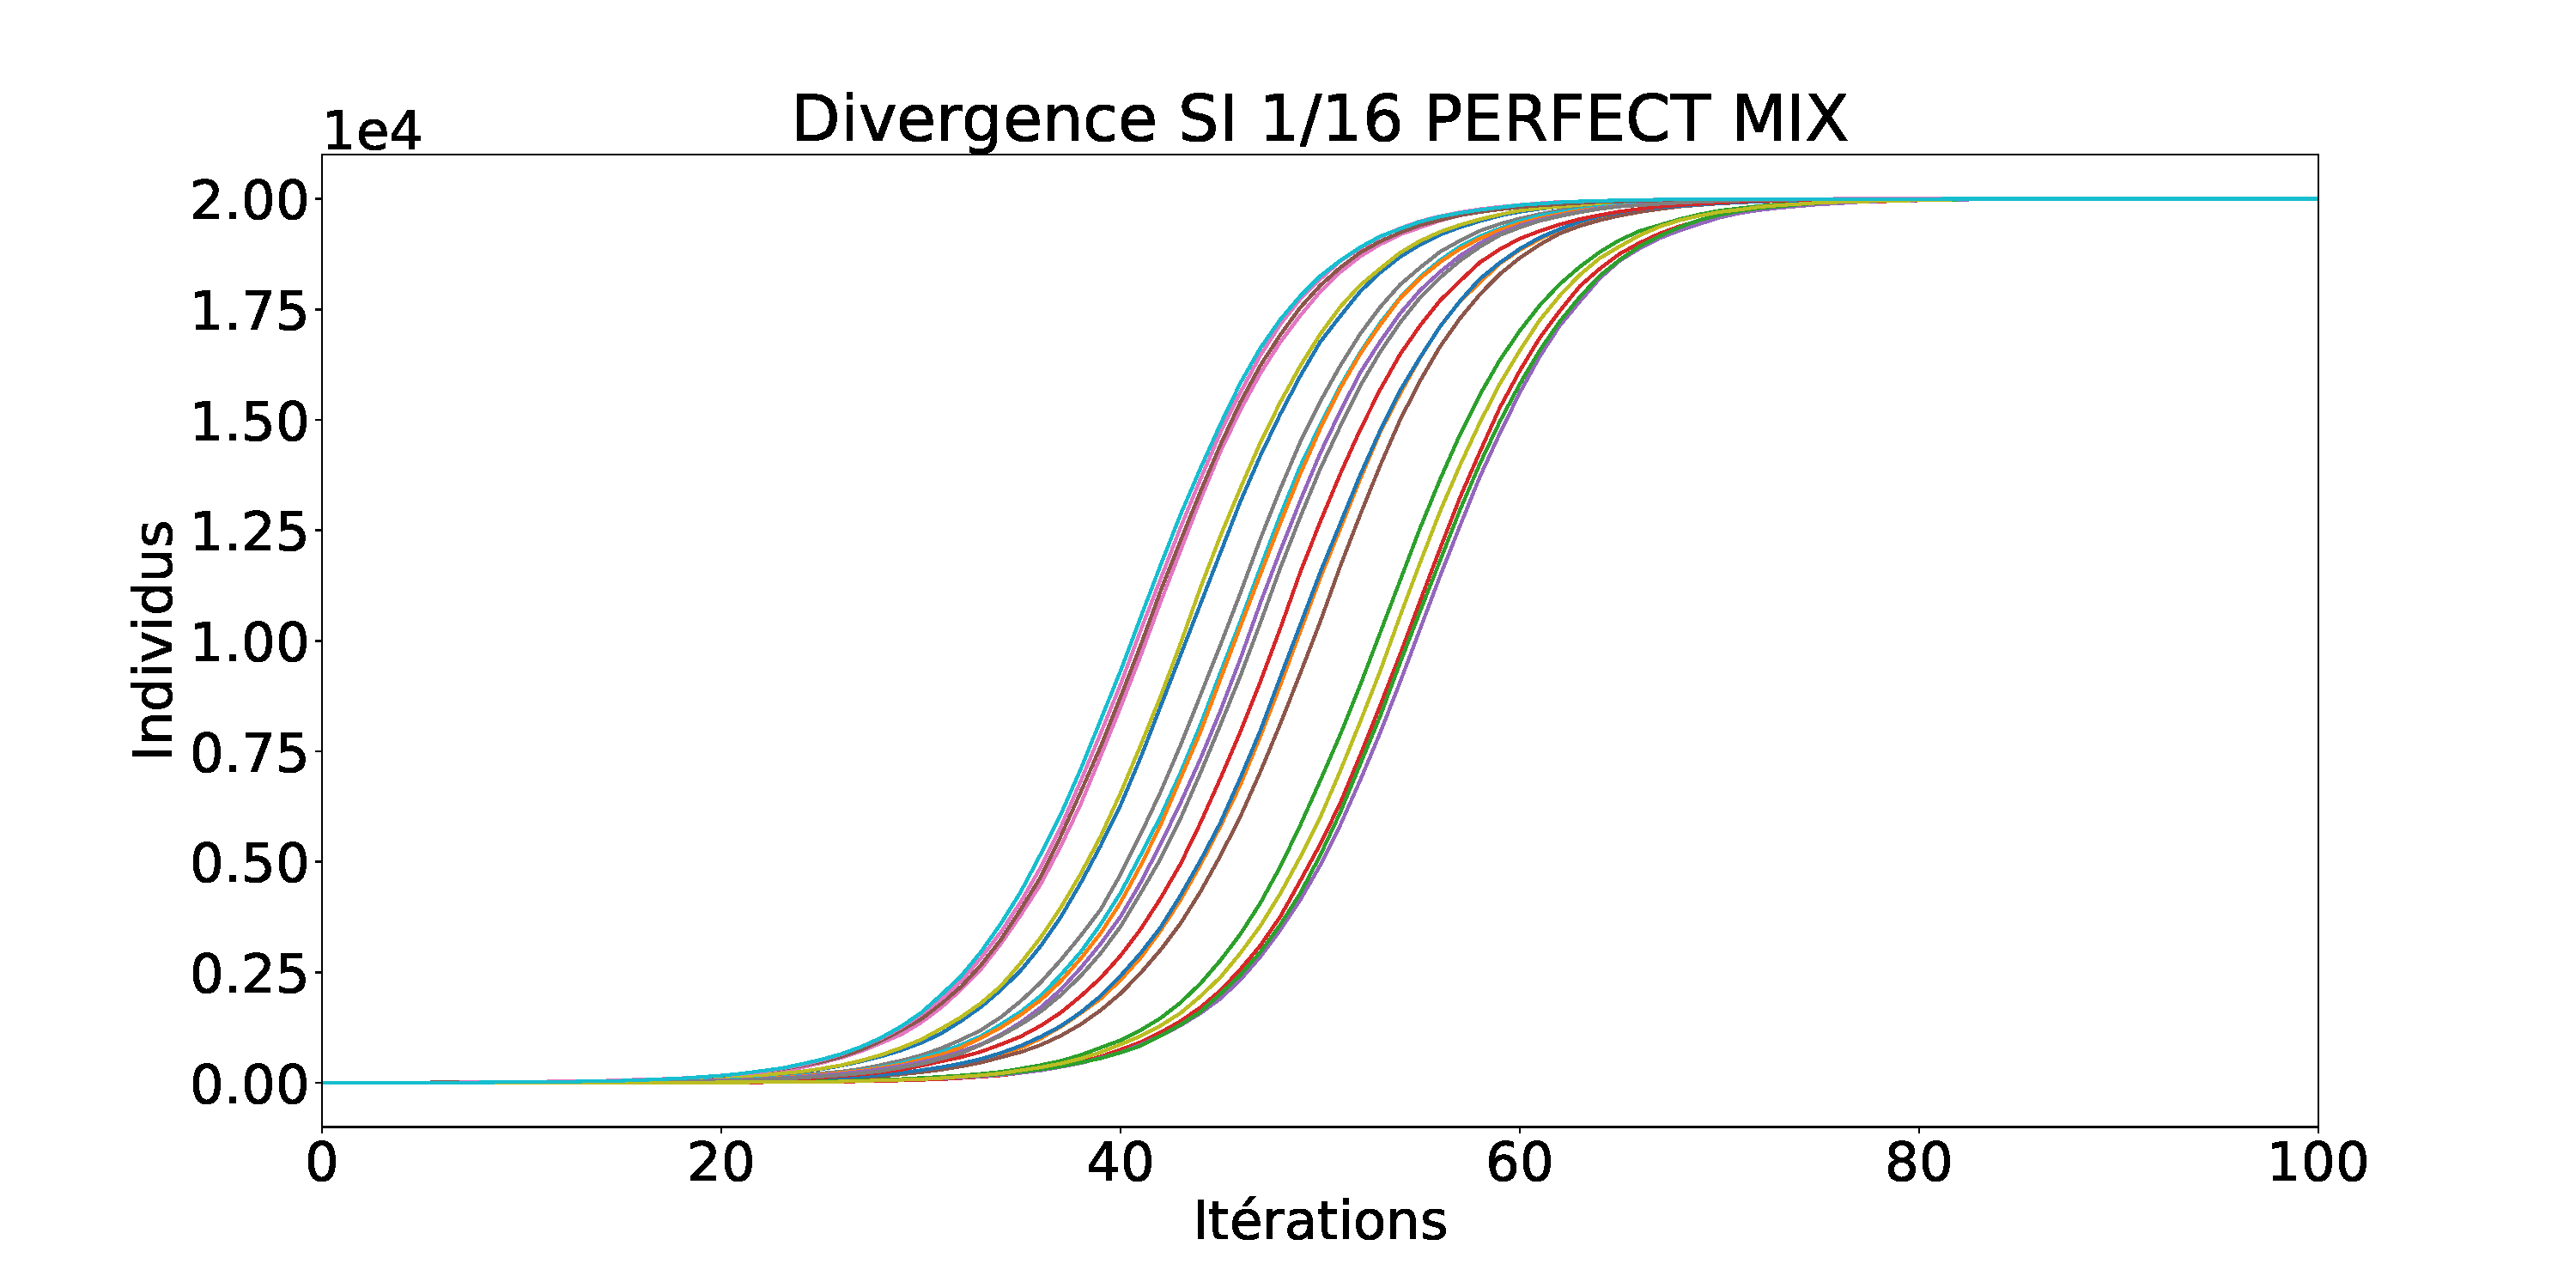
\includegraphics[width=0.5\textwidth]{Images/SI_divergence_16_mix.pdf}
    \caption{Variations SI}
\end{wrapfigure}

Sur chacune des figure sont représentées les $20$ simulations aux mêmes paramètres. Les mesures effectuées sur les simulations permettent de mettre ces courbes en relations les unes avec les autres. L'intérêt des mesures est de calculer les décalages sur l'axe des abscisses. Pour ce faire nous mesurons à quelle itération la moitié du système est contaminé. Les simulations ont toutes un nombre d'individus de $20000$ par conséquent nous mesurons à quelle itérations les simulations ont atteint $10000$ infectés. C'est à cet endroit que les déviations sont les plus grandes. En effectuant la même mesure en calculant l'itération des $20000$ infectés, nous obtenons des variations moins importantes.\\

Avec les mesures nous pouvons calculer l'itération minimale ainsi que l'itération maximale des simulations pour atteindre le seuil des $10000$ individus infectés. Il est ensuite possible de calculer la moyenne et la moyenne des déviations à cette moyenne.

\begin{table}[H]
\centering
\captionsetup{justification=centering}
\caption[Variations : SI]{Variations : modèle SI\label{tab:grid}}
\begin{tabular}{@{\extracolsep{\fill} } c|| c| c| c| c|}
 & \multicolumn{2}{|c|}{1000 mouvements} & \multicolumn{2}{|c|}{Mélange parfait} \\
\midrule
\midrule
densité & 1/8 & 1/16 & 1/8 & 1/16\\
\midrule
min & $24$ & $42$ & $22$ & $41$\\
\midrule
max & $32$ & $64$ & $37$ & $55$\\
\midrule
mean & $26.9$ & $50.15$ & $25.1$ & $47.7$\\
\midrule
std & $2.52$ & $5.81$ & $3.27$ & $4.63$\\
\bottomrule
\end{tabular}
\end{table}

Plus les systèmes sont grands et plus les variations sont grandes comme on peut le voir dans les résultats. Les simulations en densité $\frac{1}{16}$ ont en moyenne une plus grande déviation ainsi qu'une plus grande différence entre le minimum et le maximum.

\subsection{Positions des individus}

Cette section a pour but de visualiser l'impacte de la densité des systèmes sur les déplacements des individus et donc sur la qualité du mélange. Les figures suivantes montrent les positions géographiques de tous les individus à une certaine itération. En vert sont affichés les individus sains et en rouge les individus contaminés.\\

L'image ci-dessous montre les positions des individus pour une simulation au mélange parfait à l'itération $7$. Le mode de mélange parfait redistribue tous les individus dans l'espace à chaque itération, par conséquent les individus contaminés sont parfaitement répartis dans l'espace.

\begin{figure}[h]
	\centering
	\captionsetup{justification=centering}
	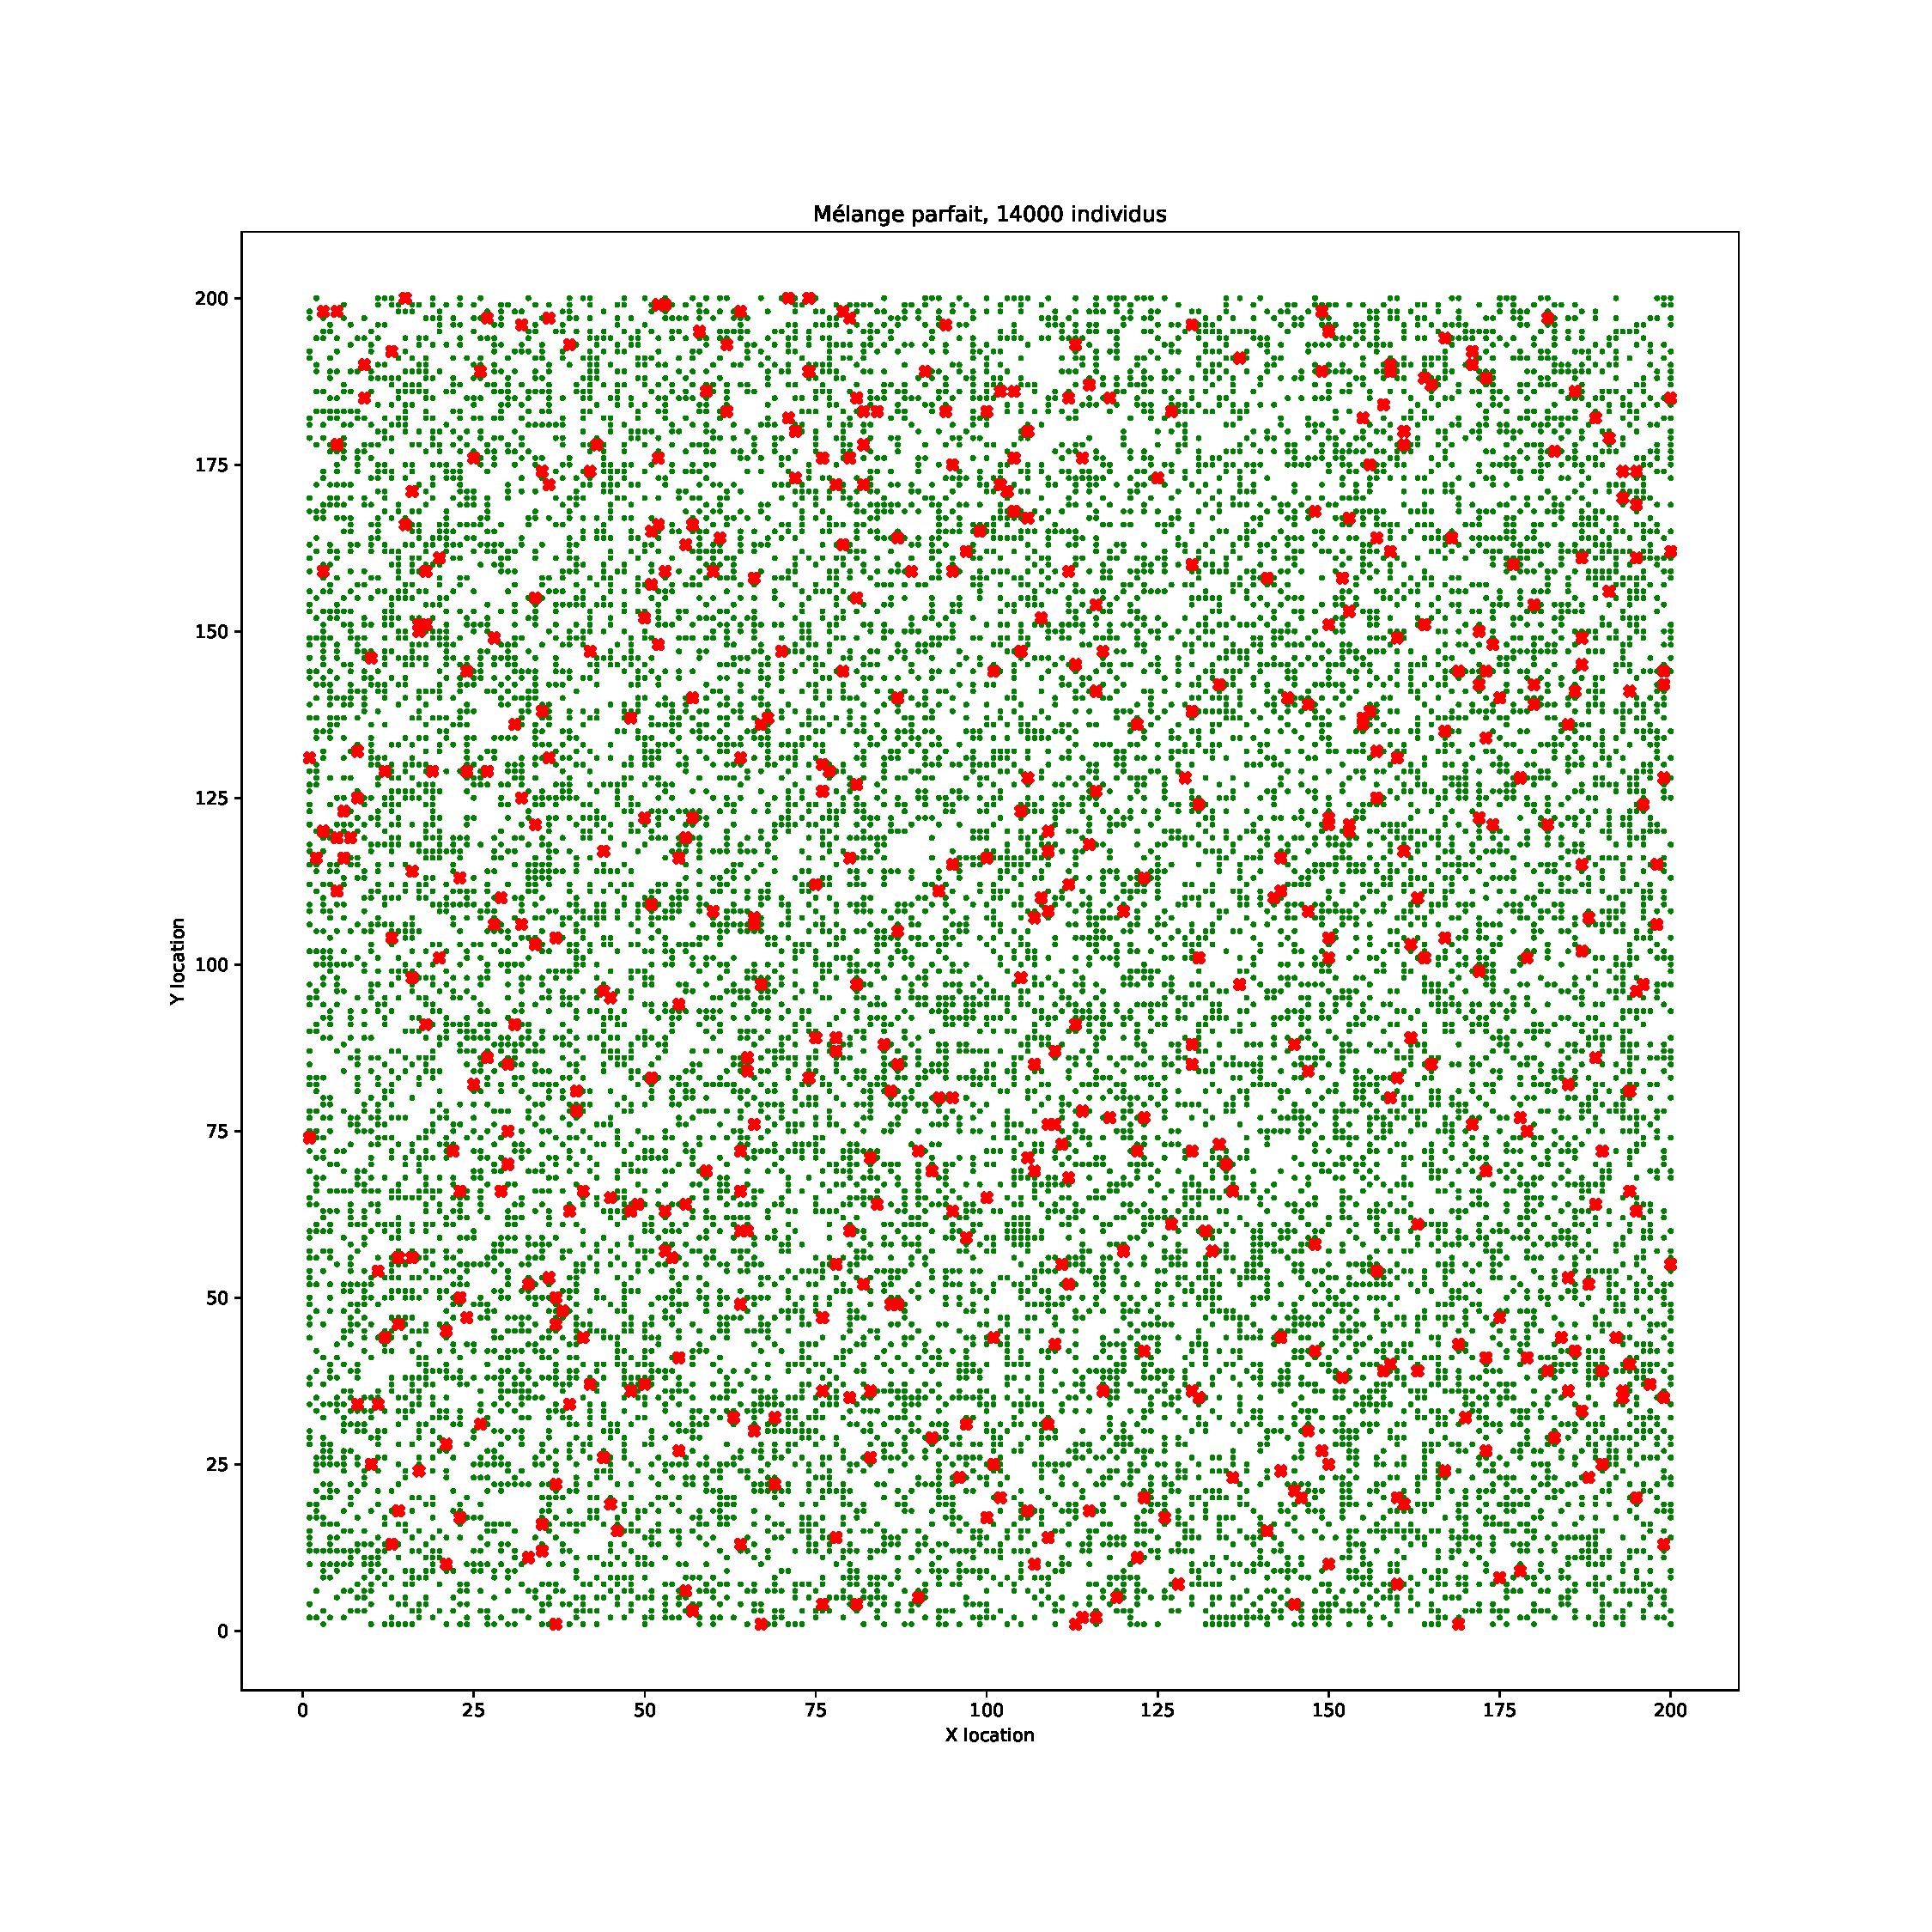
\includegraphics[width=.7\textwidth]{Images/SI_positions_14k_mix.pdf}
	\caption{positions, mélange parfait}
\end{figure}

\newpage

Sur les figures qui suivent, nous effectuons la même mesure mais cette fois-ci sur des simulations aux $1000$ mouvements. Le nombre d'individus est de $10000$, $14000$, $17000$ et $20000$ nous onvons donc quatre simulations aux densité différentes mais paramétrées de manière identique. L'idée est de pouvoir observer la qualité du mélange de la population en fonction de la densité du système.

\begin{figure}[h]
	\centering
	\captionsetup{justification=centering}
	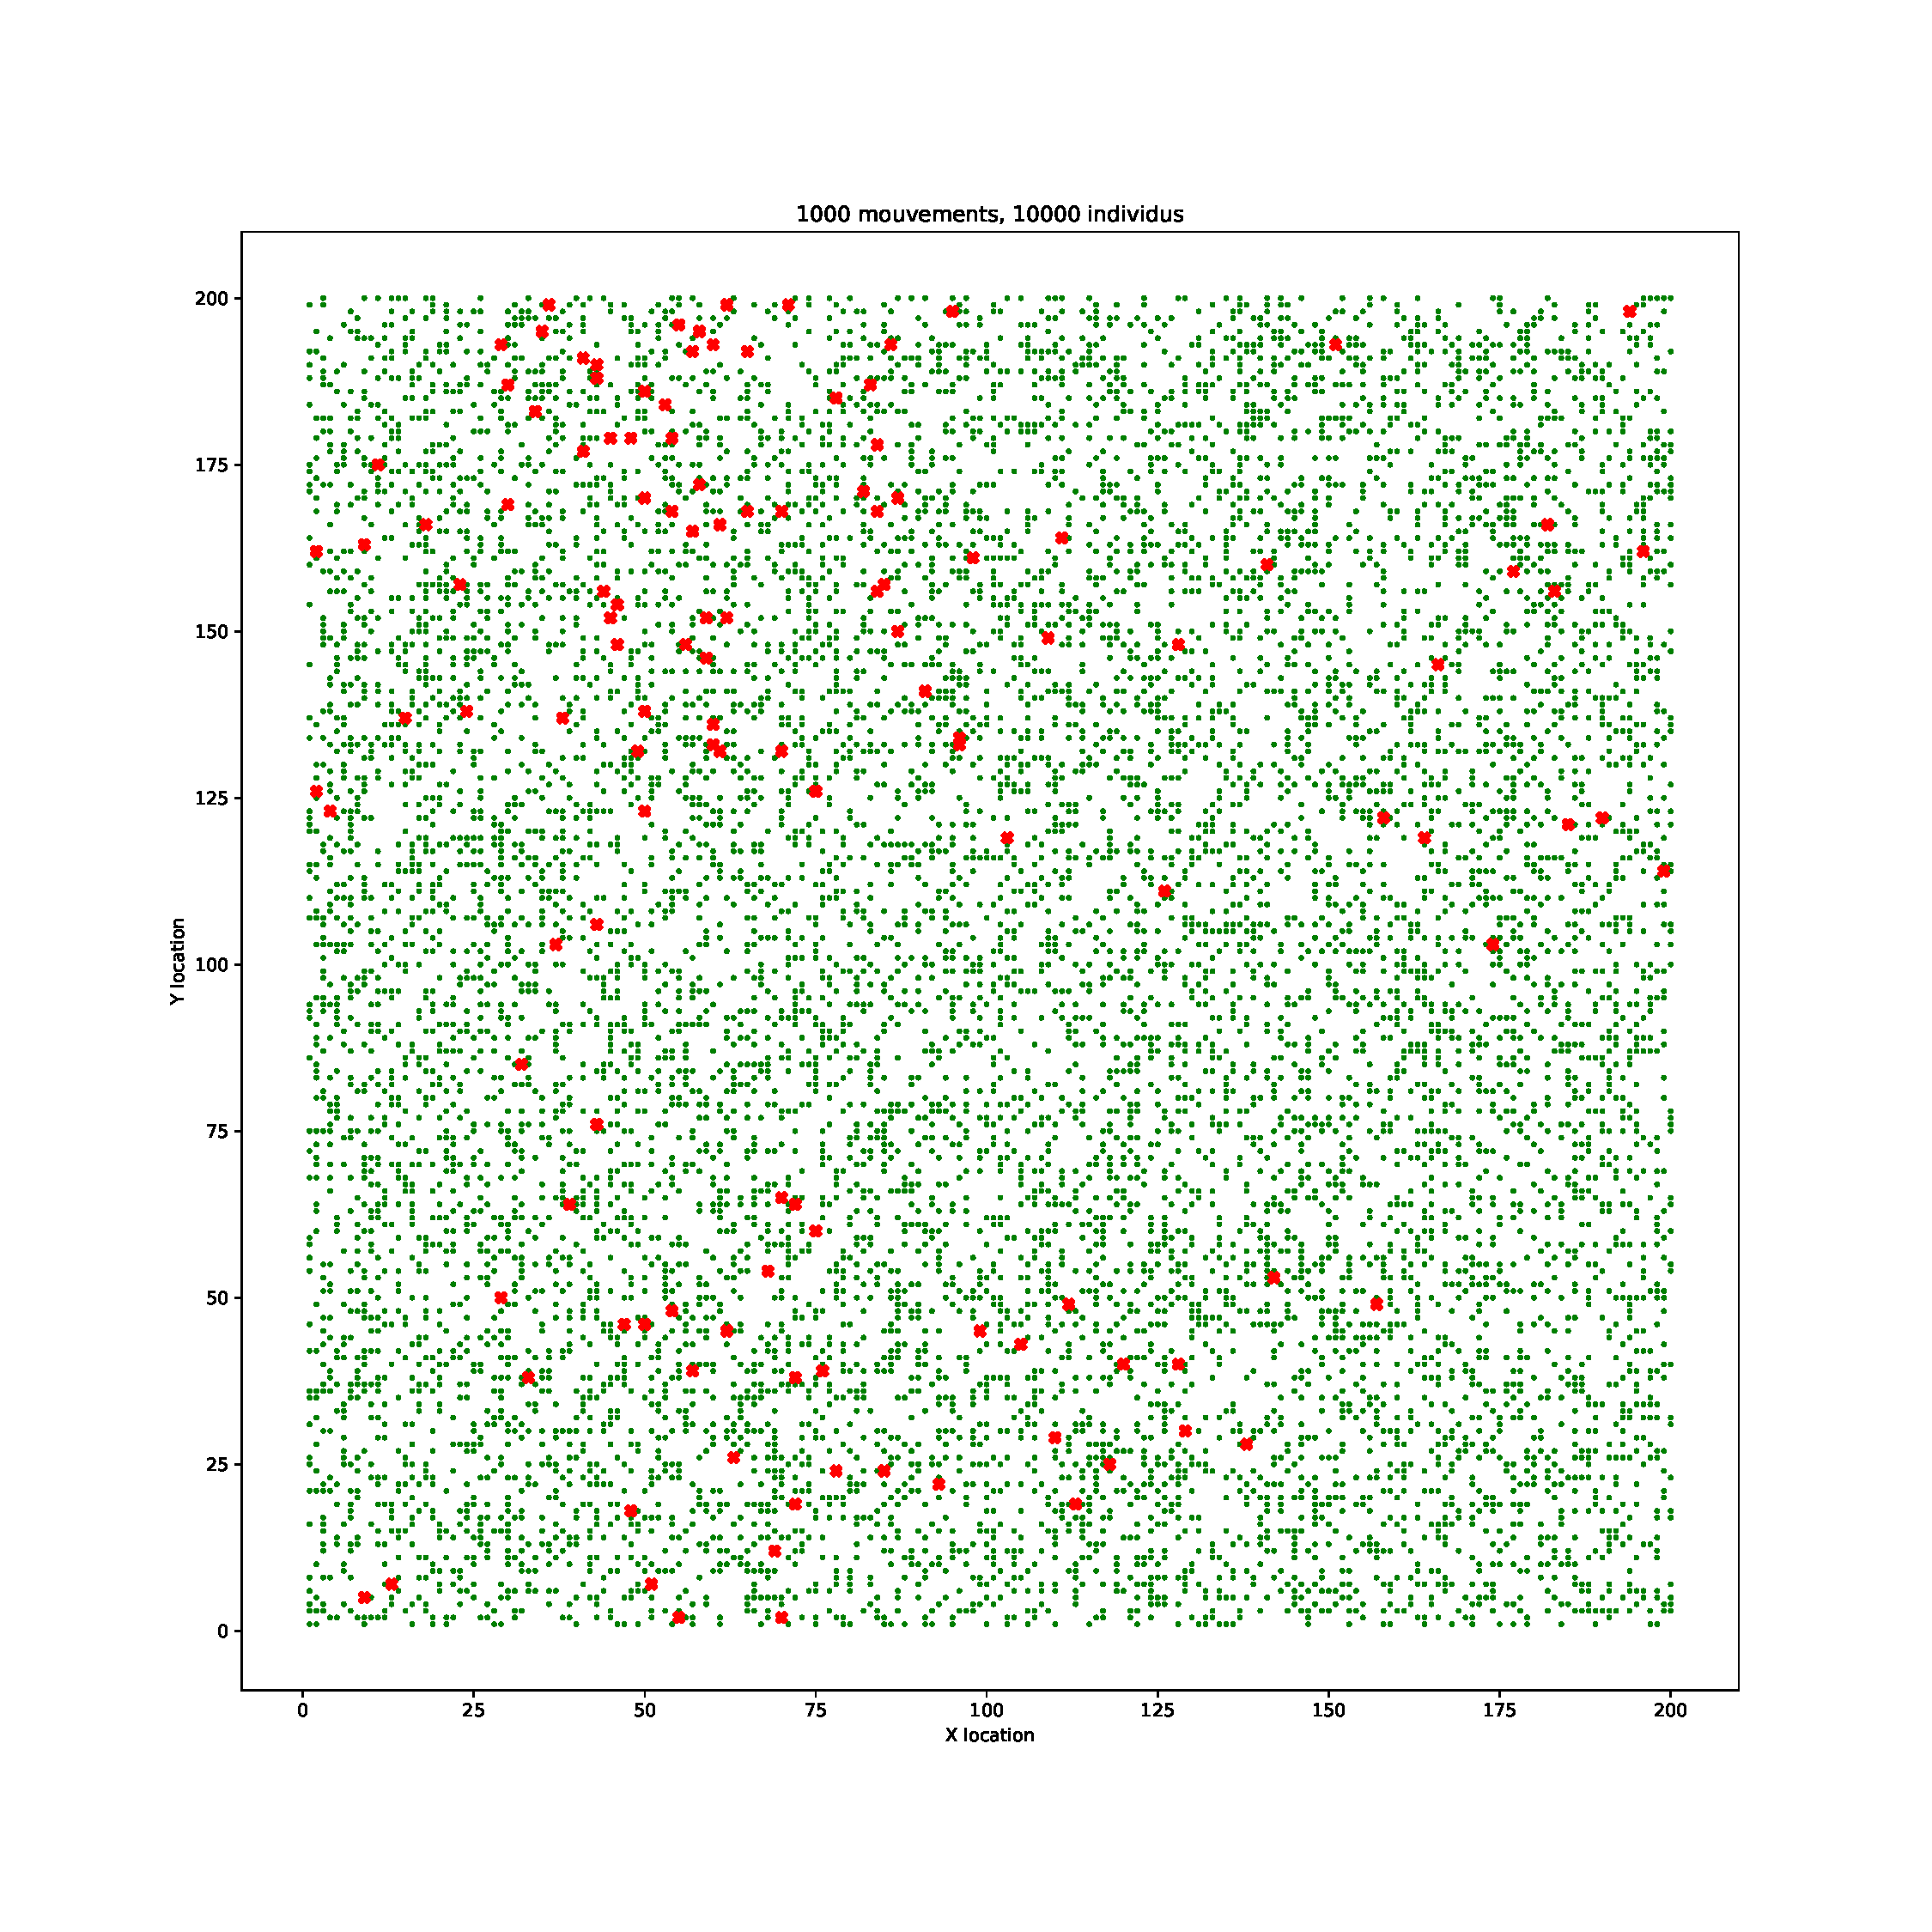
\includegraphics[width=.4\textwidth]{Images/SI_positions_10k.pdf}
	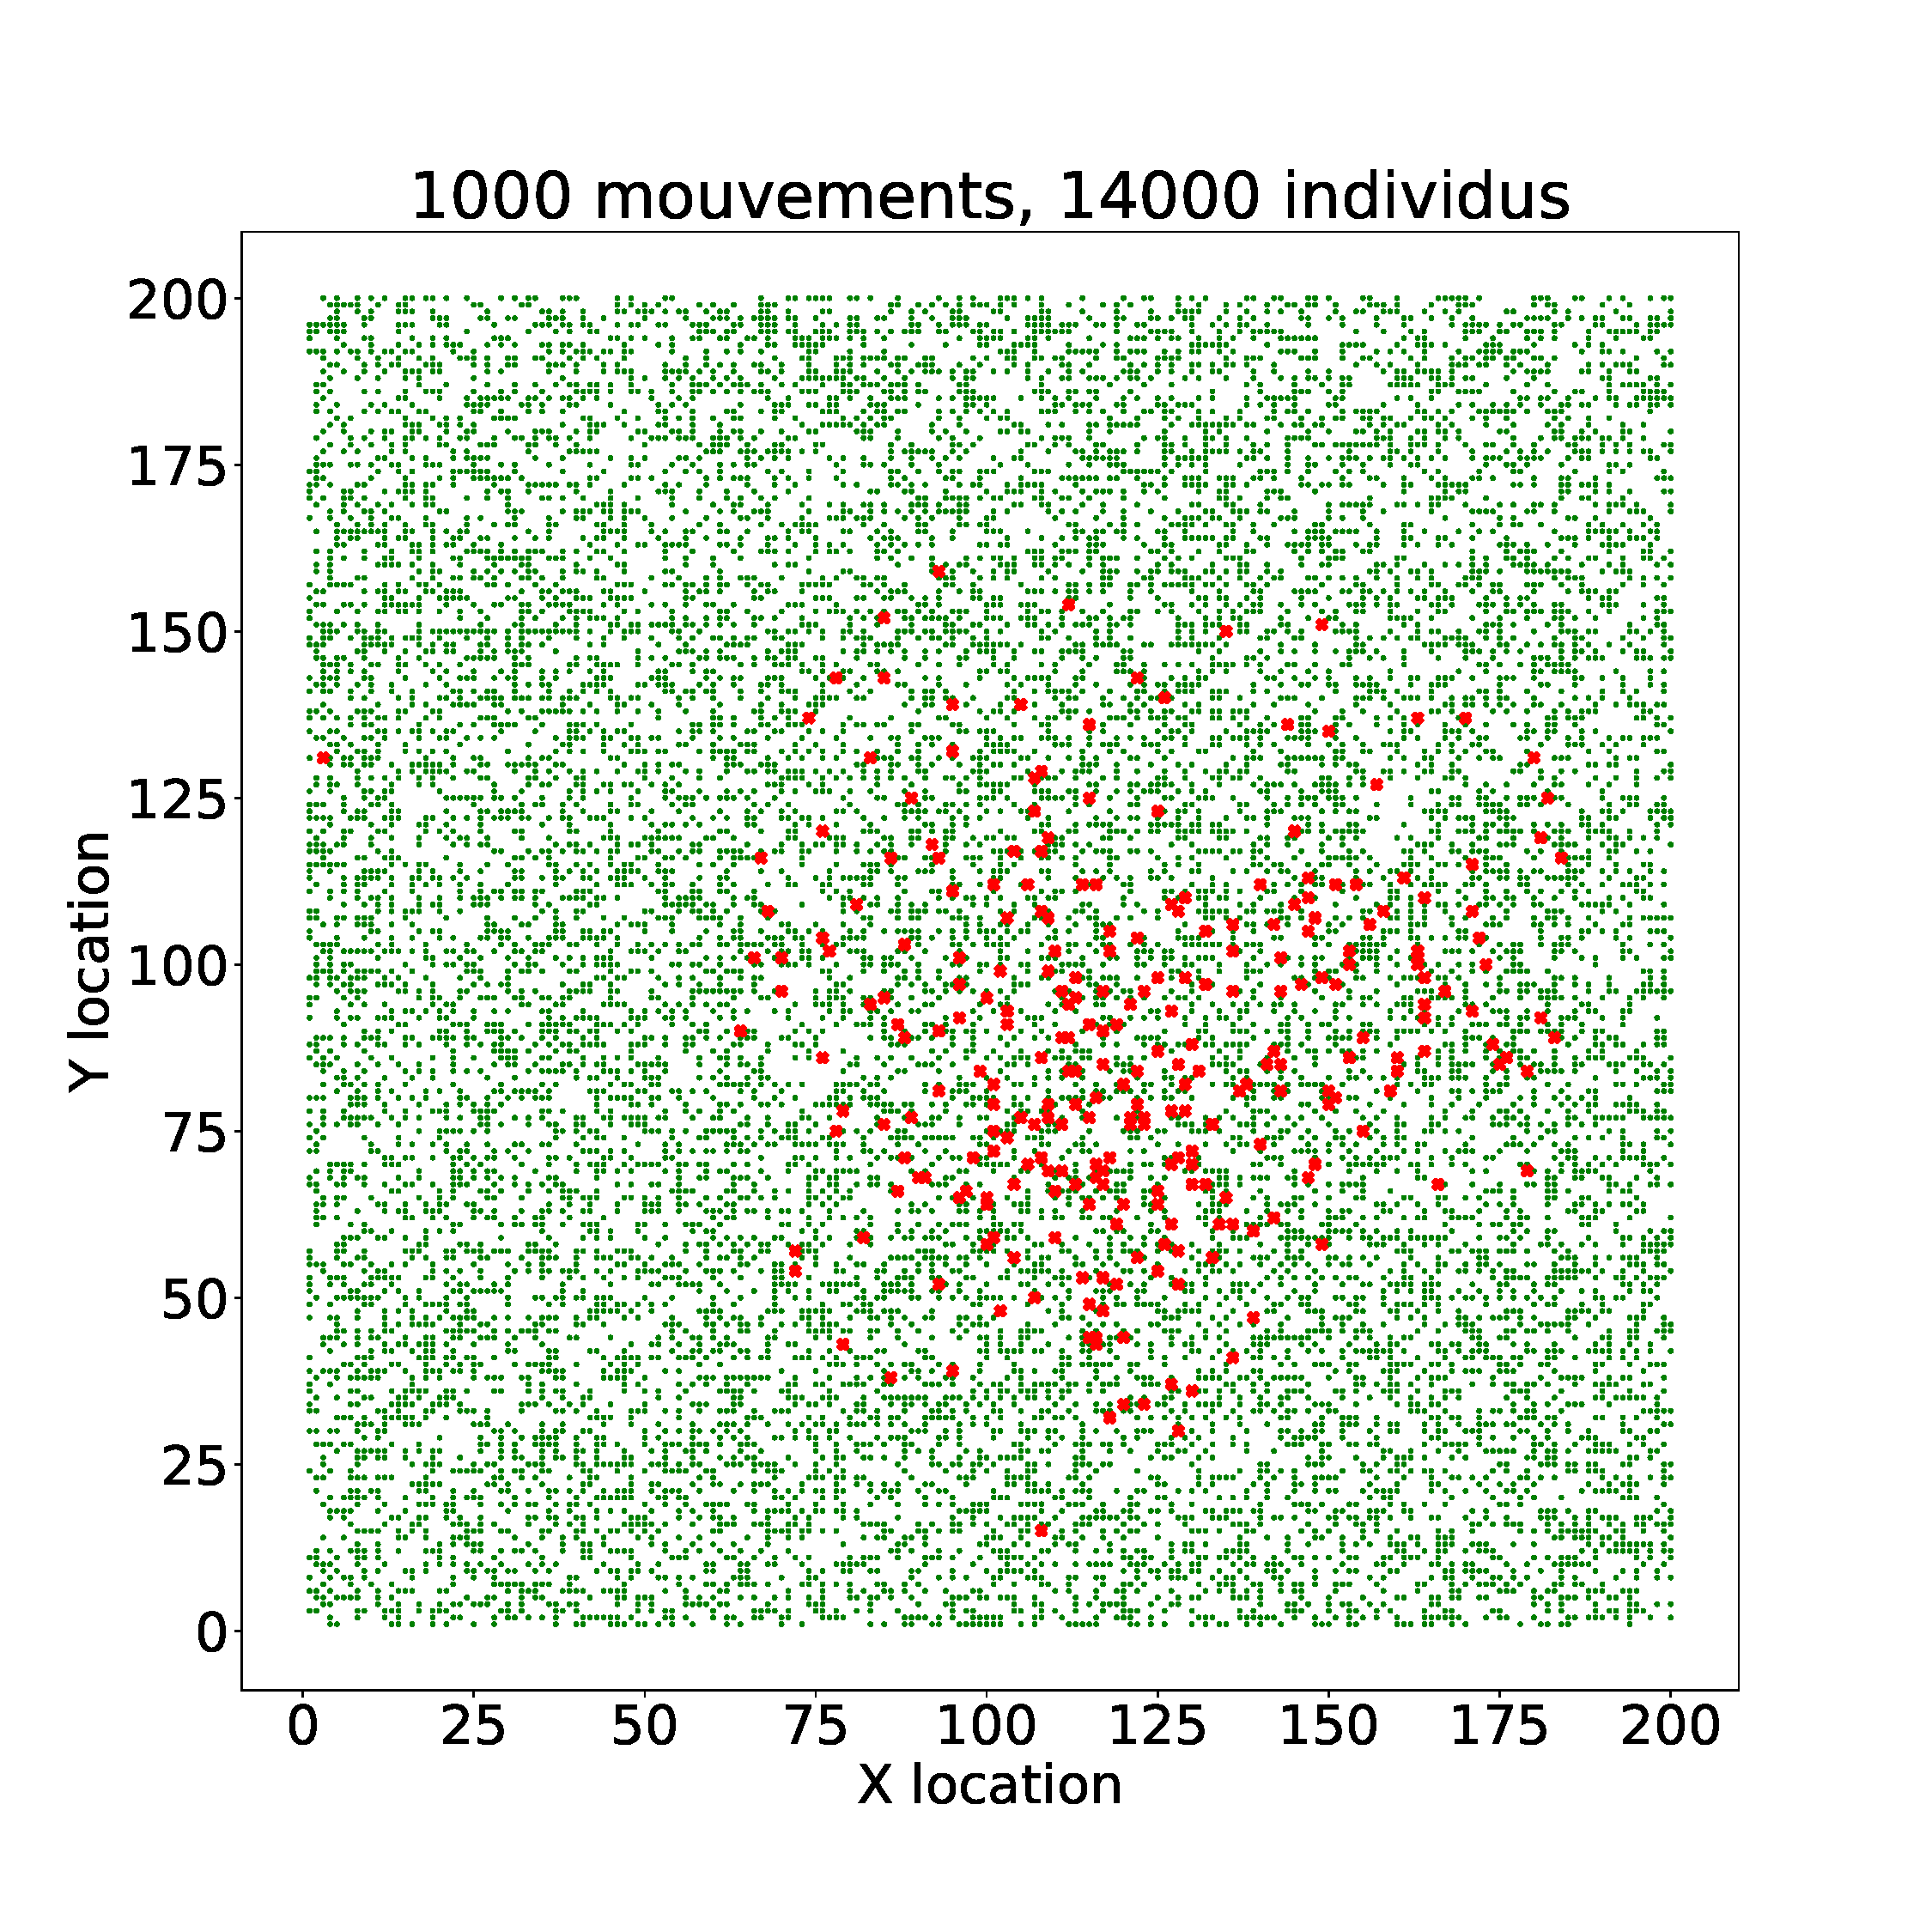
\includegraphics[width=.4\textwidth]{Images/SI_positions_14k.pdf}
	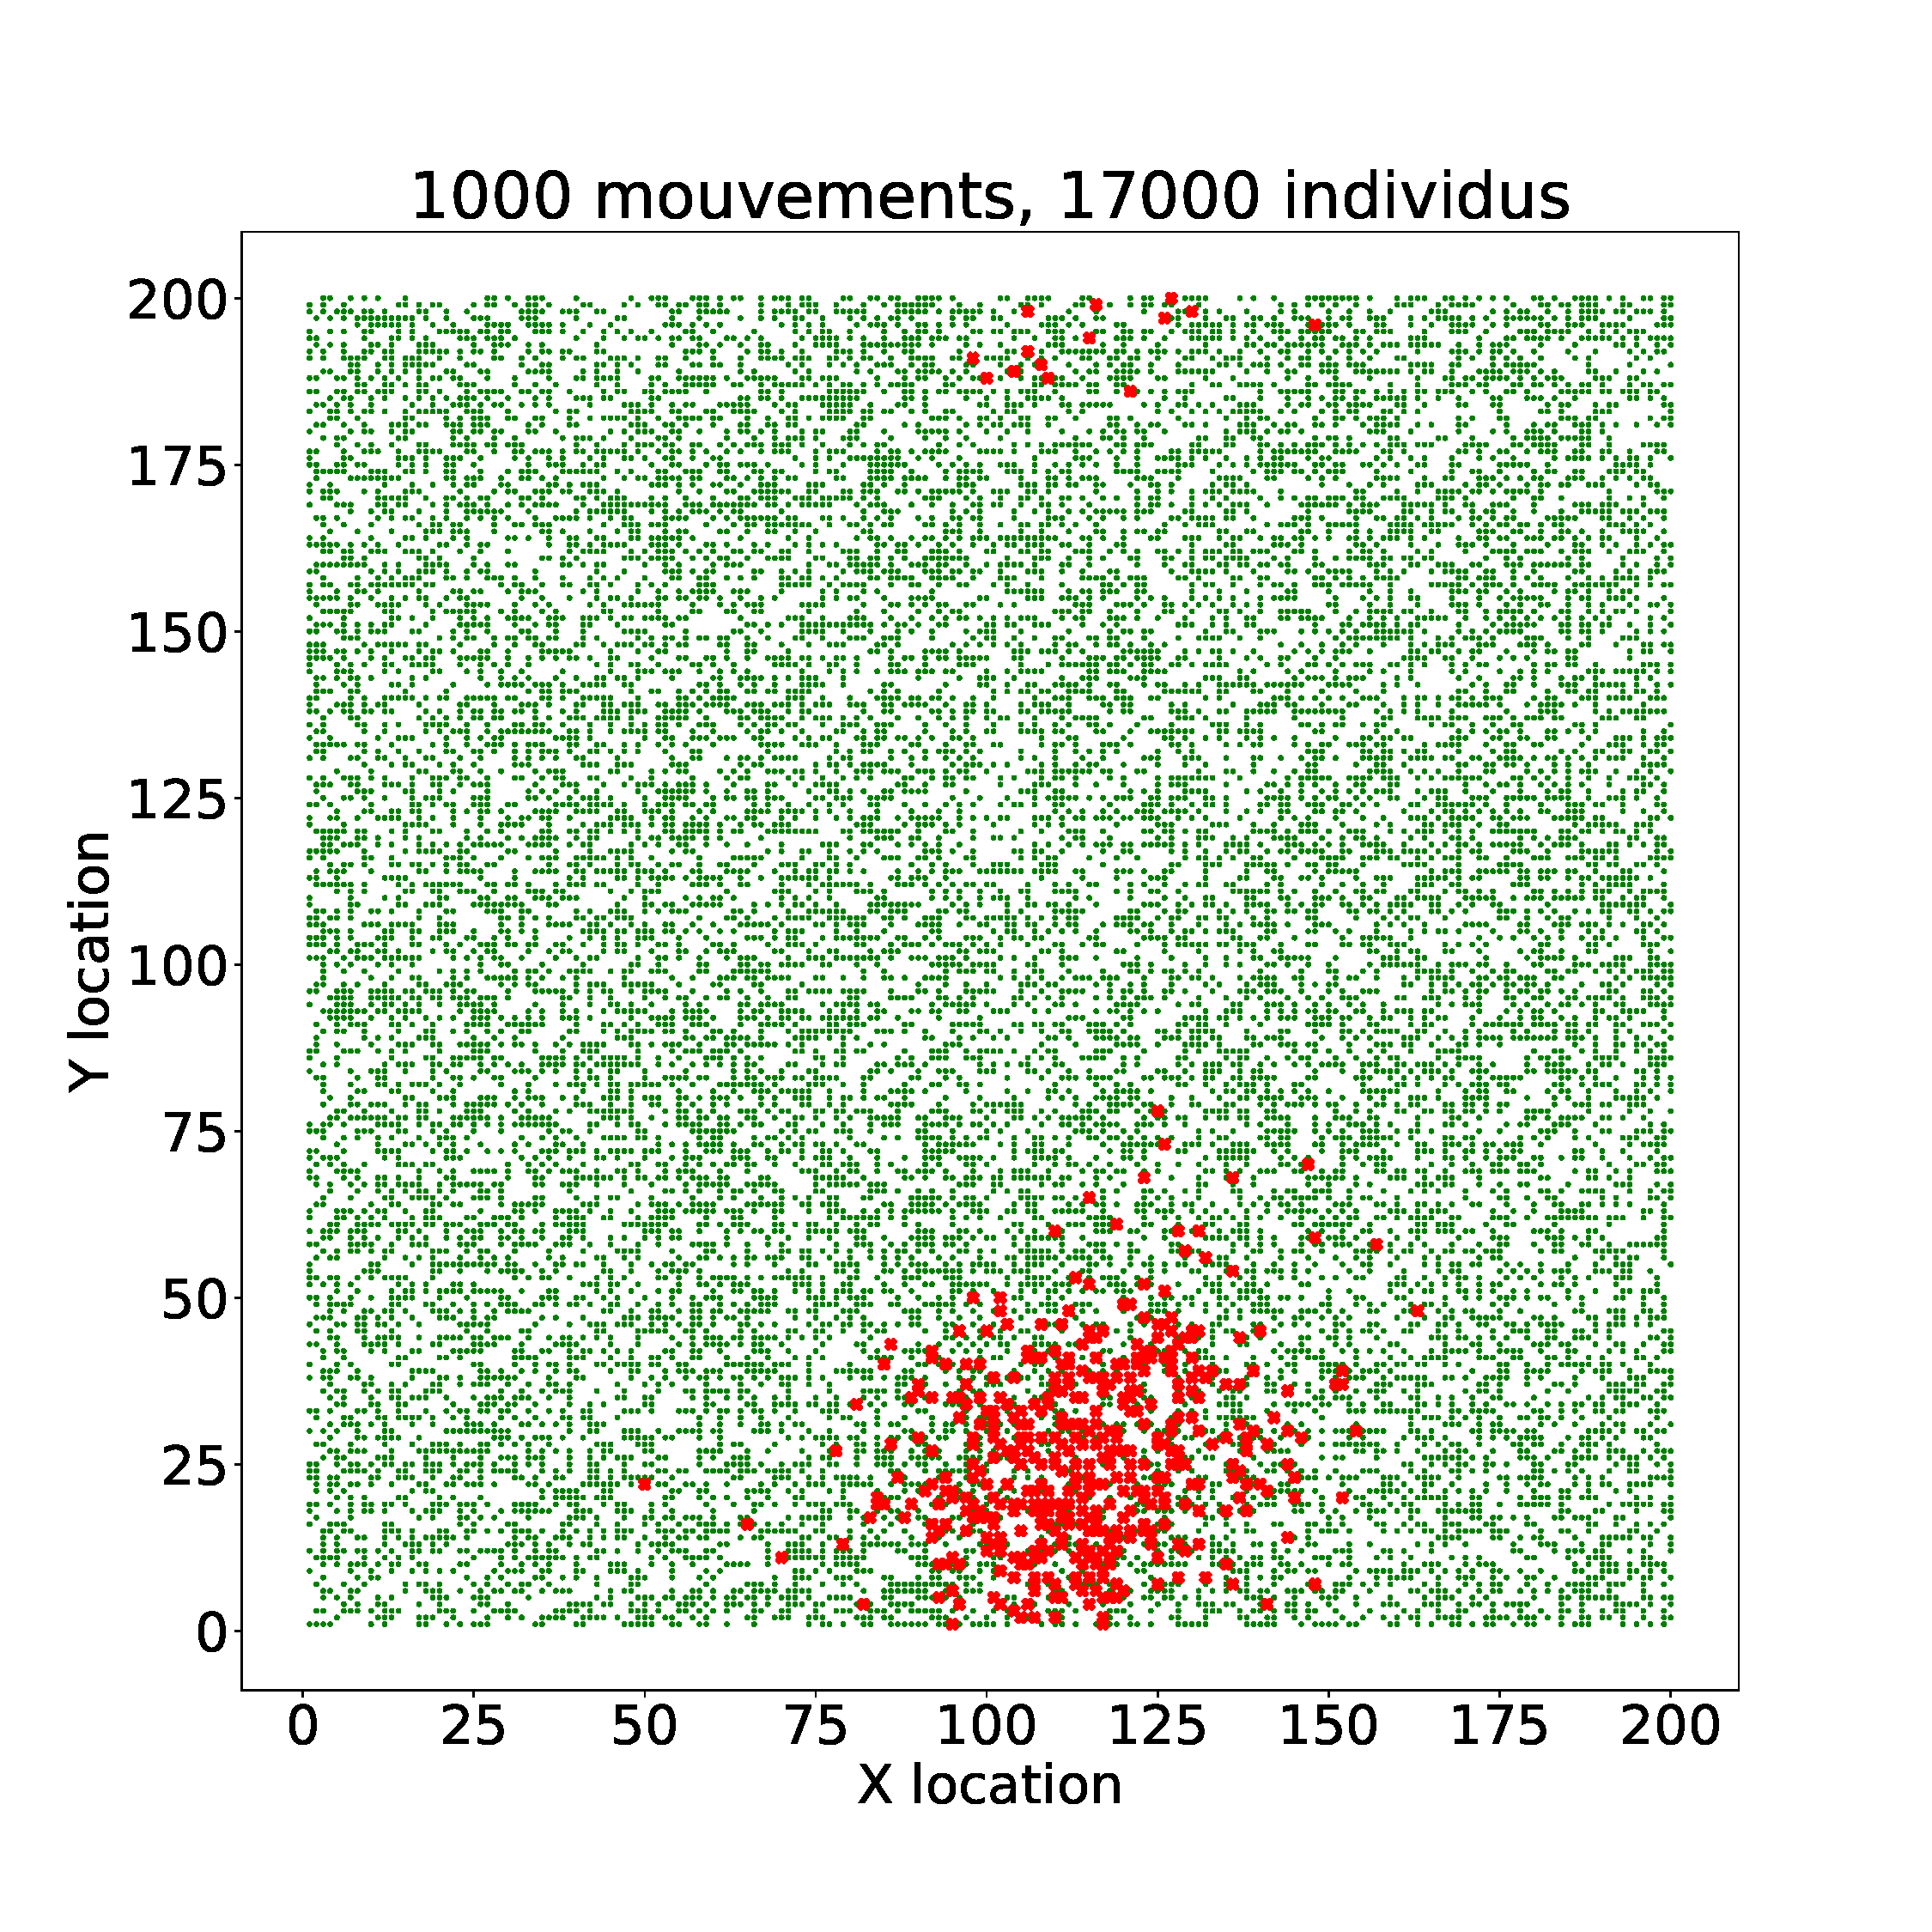
\includegraphics[width=.4\textwidth]{Images/SI_positions_17k.pdf}
	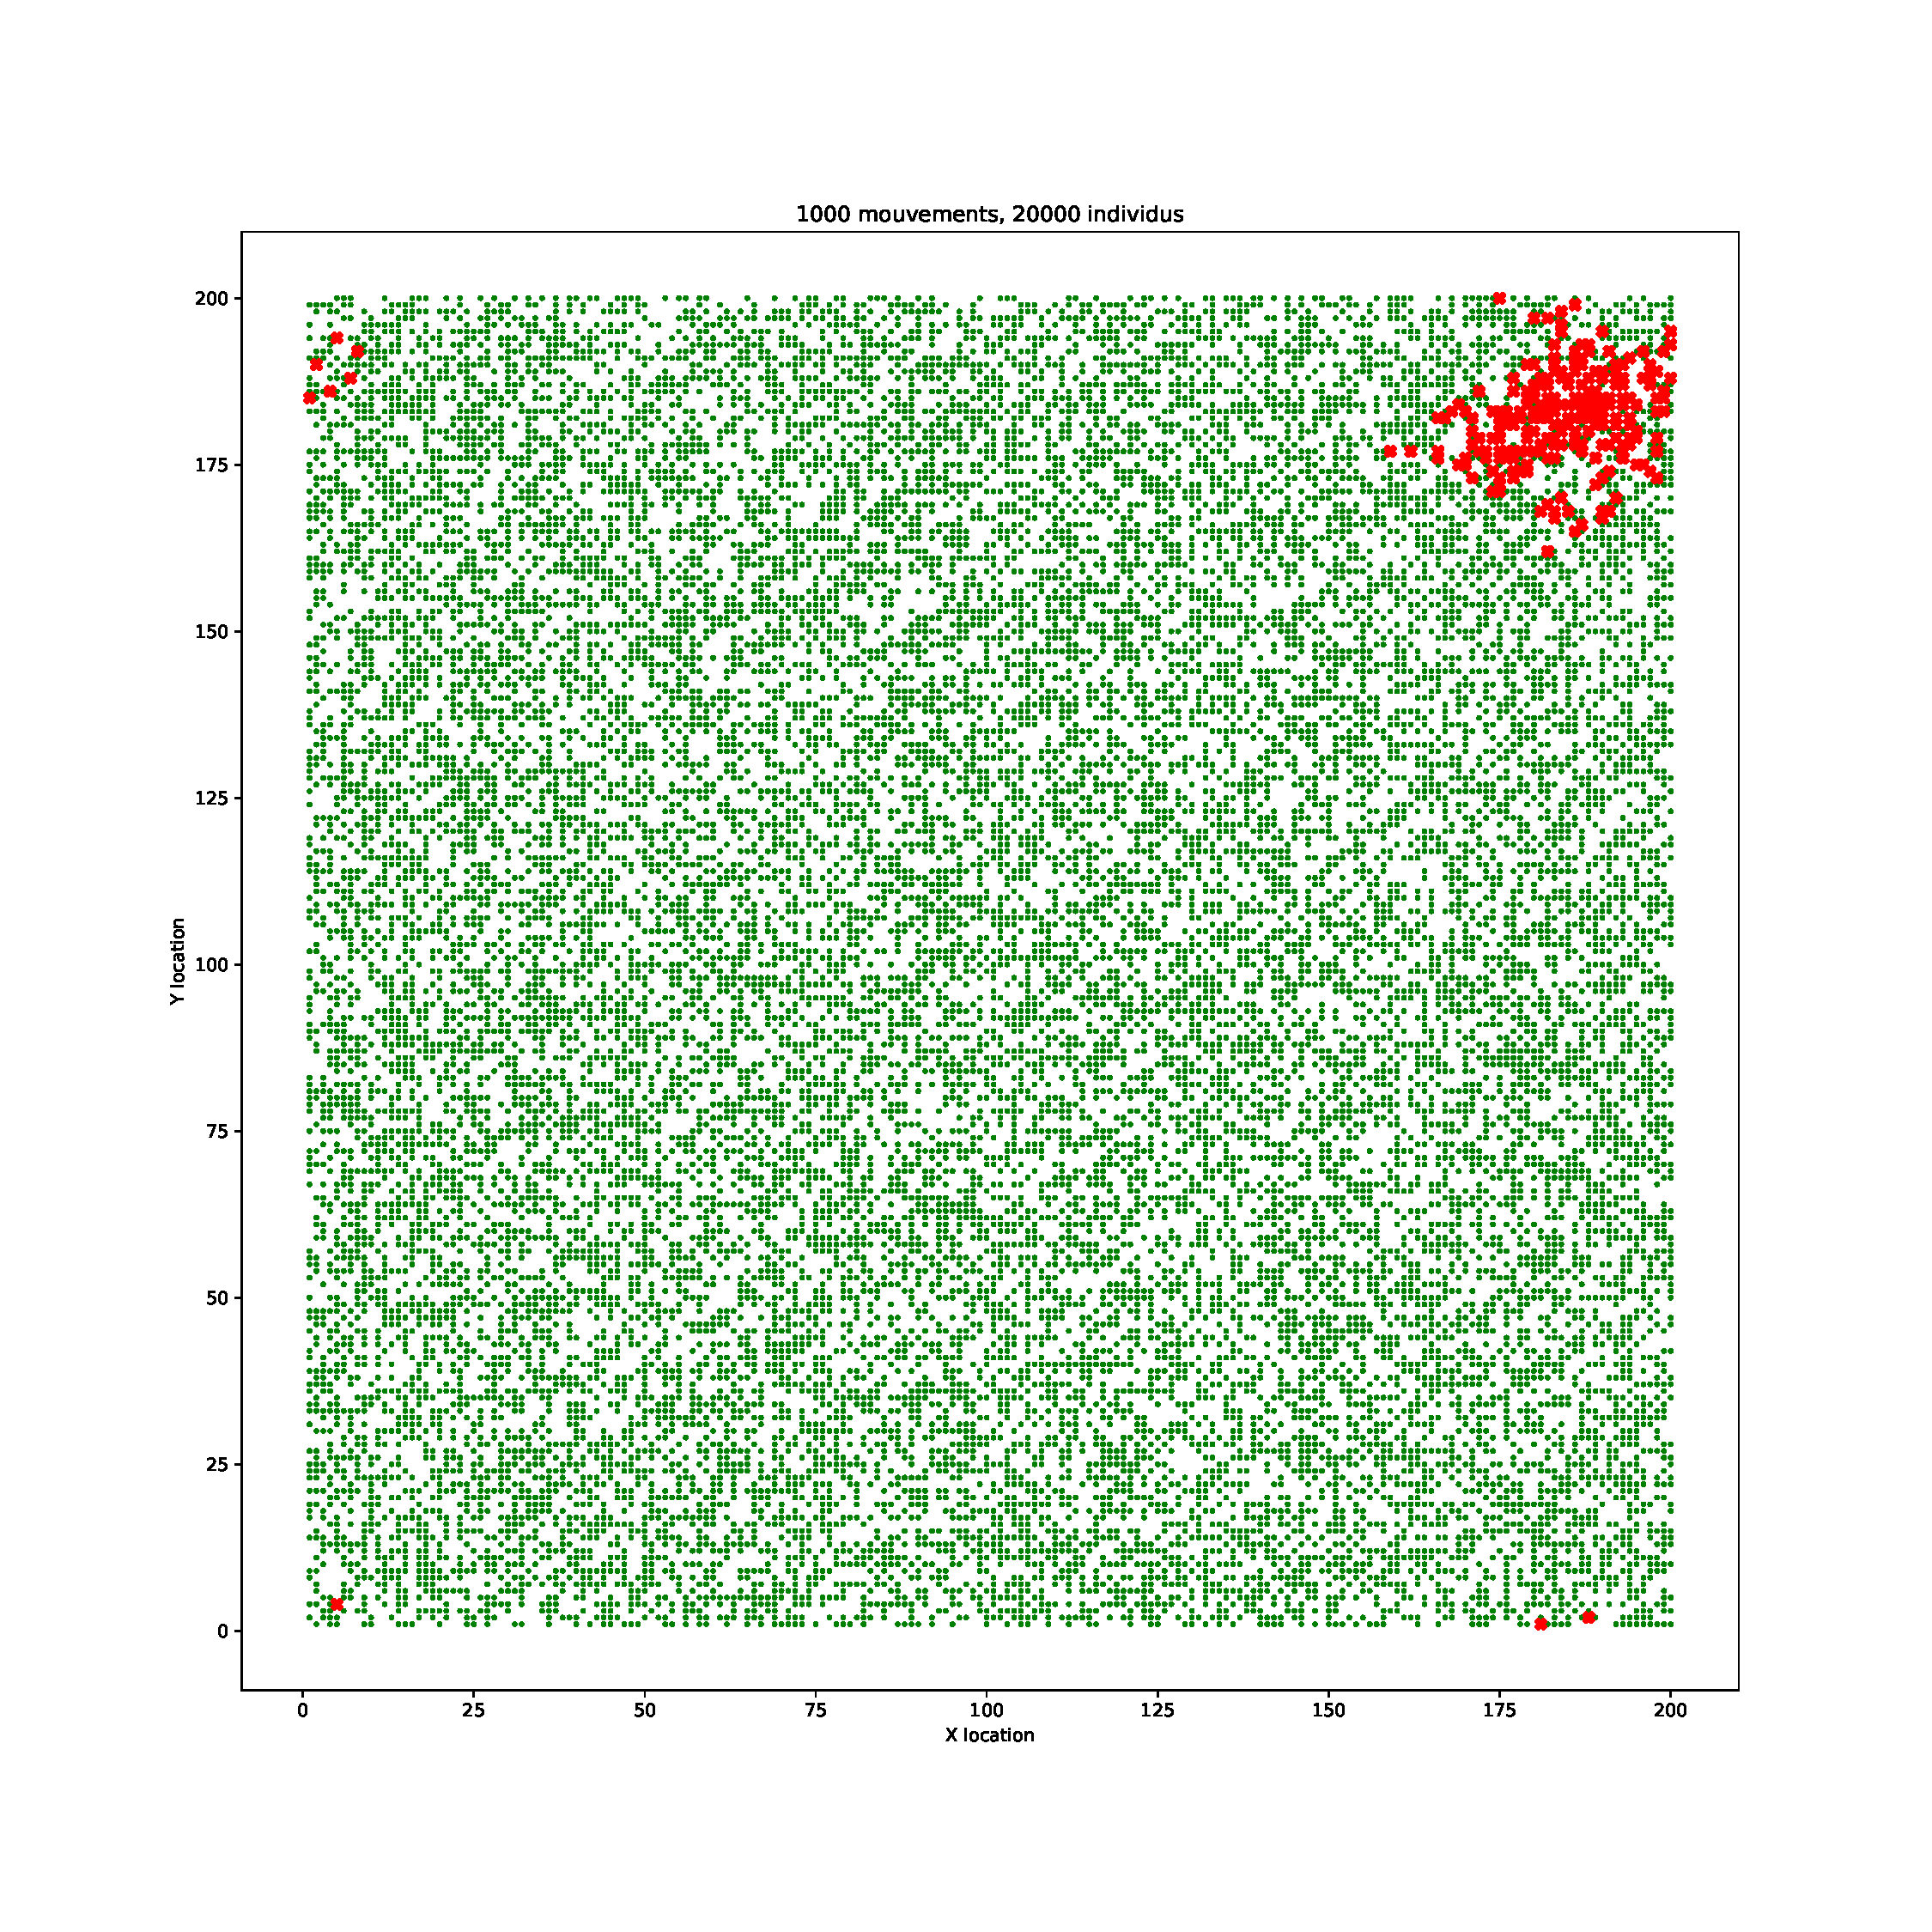
\includegraphics[width=.4\textwidth]{Images/SI_positions_20k.pdf}
	\caption{positions, 1000 mouvements}
\end{figure}

Afin de pouvoir comparer les simulations, nous avons fixé la taille du système à $200 \times 200$ et faisons varier uniquement le nombre d'individus. La dispersion des individus confime le fait que les mouvements sont entravés dans les simulations aux $1000$ mouvements. Pour rappel, en mode $1000$ mouvements, un individu essaie de se déplacer $1000$ fois par itération mais si le passage est obstrué, l'individu ne se déplace pas et ceci est compatibilisé comme mouvement.\\

Par conséquent, le diamètre de propagation croit avec la diminution de la densité du système. 